% Options for packages loaded elsewhere
\PassOptionsToPackage{unicode}{hyperref}
\PassOptionsToPackage{hyphens}{url}
%
\documentclass[
]{article}
\usepackage{amsmath,amssymb}
\usepackage{lmodern}
\usepackage{iftex}
\ifPDFTeX
  \usepackage[T1]{fontenc}
  \usepackage[utf8]{inputenc}
  \usepackage{textcomp} % provide euro and other symbols
\else % if luatex or xetex
  \usepackage{unicode-math}
  \defaultfontfeatures{Scale=MatchLowercase}
  \defaultfontfeatures[\rmfamily]{Ligatures=TeX,Scale=1}
\fi
% Use upquote if available, for straight quotes in verbatim environments
\IfFileExists{upquote.sty}{\usepackage{upquote}}{}
\IfFileExists{microtype.sty}{% use microtype if available
  \usepackage[]{microtype}
  \UseMicrotypeSet[protrusion]{basicmath} % disable protrusion for tt fonts
}{}
\makeatletter
\@ifundefined{KOMAClassName}{% if non-KOMA class
  \IfFileExists{parskip.sty}{%
    \usepackage{parskip}
  }{% else
    \setlength{\parindent}{0pt}
    \setlength{\parskip}{6pt plus 2pt minus 1pt}}
}{% if KOMA class
  \KOMAoptions{parskip=half}}
\makeatother
\usepackage{xcolor}
\IfFileExists{xurl.sty}{\usepackage{xurl}}{} % add URL line breaks if available
\IfFileExists{bookmark.sty}{\usepackage{bookmark}}{\usepackage{hyperref}}
\hypersetup{
  pdftitle={Comparing the relationship between data quality and engagement using threshold approaches vs hidden Markov models in an app-based experience sampling study},
  hidelinks,
  pdfcreator={LaTeX via pandoc}}
\urlstyle{same} % disable monospaced font for URLs
\usepackage[margin=1in]{geometry}
\usepackage{color}
\usepackage{fancyvrb}
\newcommand{\VerbBar}{|}
\newcommand{\VERB}{\Verb[commandchars=\\\{\}]}
\DefineVerbatimEnvironment{Highlighting}{Verbatim}{commandchars=\\\{\}}
% Add ',fontsize=\small' for more characters per line
\usepackage{framed}
\definecolor{shadecolor}{RGB}{248,248,248}
\newenvironment{Shaded}{\begin{snugshade}}{\end{snugshade}}
\newcommand{\AlertTok}[1]{\textcolor[rgb]{0.94,0.16,0.16}{#1}}
\newcommand{\AnnotationTok}[1]{\textcolor[rgb]{0.56,0.35,0.01}{\textbf{\textit{#1}}}}
\newcommand{\AttributeTok}[1]{\textcolor[rgb]{0.77,0.63,0.00}{#1}}
\newcommand{\BaseNTok}[1]{\textcolor[rgb]{0.00,0.00,0.81}{#1}}
\newcommand{\BuiltInTok}[1]{#1}
\newcommand{\CharTok}[1]{\textcolor[rgb]{0.31,0.60,0.02}{#1}}
\newcommand{\CommentTok}[1]{\textcolor[rgb]{0.56,0.35,0.01}{\textit{#1}}}
\newcommand{\CommentVarTok}[1]{\textcolor[rgb]{0.56,0.35,0.01}{\textbf{\textit{#1}}}}
\newcommand{\ConstantTok}[1]{\textcolor[rgb]{0.00,0.00,0.00}{#1}}
\newcommand{\ControlFlowTok}[1]{\textcolor[rgb]{0.13,0.29,0.53}{\textbf{#1}}}
\newcommand{\DataTypeTok}[1]{\textcolor[rgb]{0.13,0.29,0.53}{#1}}
\newcommand{\DecValTok}[1]{\textcolor[rgb]{0.00,0.00,0.81}{#1}}
\newcommand{\DocumentationTok}[1]{\textcolor[rgb]{0.56,0.35,0.01}{\textbf{\textit{#1}}}}
\newcommand{\ErrorTok}[1]{\textcolor[rgb]{0.64,0.00,0.00}{\textbf{#1}}}
\newcommand{\ExtensionTok}[1]{#1}
\newcommand{\FloatTok}[1]{\textcolor[rgb]{0.00,0.00,0.81}{#1}}
\newcommand{\FunctionTok}[1]{\textcolor[rgb]{0.00,0.00,0.00}{#1}}
\newcommand{\ImportTok}[1]{#1}
\newcommand{\InformationTok}[1]{\textcolor[rgb]{0.56,0.35,0.01}{\textbf{\textit{#1}}}}
\newcommand{\KeywordTok}[1]{\textcolor[rgb]{0.13,0.29,0.53}{\textbf{#1}}}
\newcommand{\NormalTok}[1]{#1}
\newcommand{\OperatorTok}[1]{\textcolor[rgb]{0.81,0.36,0.00}{\textbf{#1}}}
\newcommand{\OtherTok}[1]{\textcolor[rgb]{0.56,0.35,0.01}{#1}}
\newcommand{\PreprocessorTok}[1]{\textcolor[rgb]{0.56,0.35,0.01}{\textit{#1}}}
\newcommand{\RegionMarkerTok}[1]{#1}
\newcommand{\SpecialCharTok}[1]{\textcolor[rgb]{0.00,0.00,0.00}{#1}}
\newcommand{\SpecialStringTok}[1]{\textcolor[rgb]{0.31,0.60,0.02}{#1}}
\newcommand{\StringTok}[1]{\textcolor[rgb]{0.31,0.60,0.02}{#1}}
\newcommand{\VariableTok}[1]{\textcolor[rgb]{0.00,0.00,0.00}{#1}}
\newcommand{\VerbatimStringTok}[1]{\textcolor[rgb]{0.31,0.60,0.02}{#1}}
\newcommand{\WarningTok}[1]{\textcolor[rgb]{0.56,0.35,0.01}{\textbf{\textit{#1}}}}
\usepackage{longtable,booktabs,array}
\usepackage{calc} % for calculating minipage widths
% Correct order of tables after \paragraph or \subparagraph
\usepackage{etoolbox}
\makeatletter
\patchcmd\longtable{\par}{\if@noskipsec\mbox{}\fi\par}{}{}
\makeatother
% Allow footnotes in longtable head/foot
\IfFileExists{footnotehyper.sty}{\usepackage{footnotehyper}}{\usepackage{footnote}}
\makesavenoteenv{longtable}
\usepackage{graphicx}
\makeatletter
\def\maxwidth{\ifdim\Gin@nat@width>\linewidth\linewidth\else\Gin@nat@width\fi}
\def\maxheight{\ifdim\Gin@nat@height>\textheight\textheight\else\Gin@nat@height\fi}
\makeatother
% Scale images if necessary, so that they will not overflow the page
% margins by default, and it is still possible to overwrite the defaults
% using explicit options in \includegraphics[width, height, ...]{}
\setkeys{Gin}{width=\maxwidth,height=\maxheight,keepaspectratio}
% Set default figure placement to htbp
\makeatletter
\def\fps@figure{htbp}
\makeatother
\setlength{\emergencystretch}{3em} % prevent overfull lines
\providecommand{\tightlist}{%
  \setlength{\itemsep}{0pt}\setlength{\parskip}{0pt}}
\setcounter{secnumdepth}{-\maxdimen} % remove section numbering
\ifLuaTeX
  \usepackage{selnolig}  % disable illegal ligatures
\fi

\title{Comparing the relationship between data quality and engagement
using threshold approaches vs hidden Markov models in an app-based
experience sampling study}
\author{}
\date{\vspace{-2.5em}}

\begin{document}
\maketitle
\begin{abstract}
Researchers in the social sciences are increasingly drawing upon citizen
science approaches for the collection of data. These approaches seek to
involve non-professional scientists in the research process.

However, there are concerns surrounding the quality of data produced by
citizen scientists, which hinder further adoption of citizen science
approaches. Protocols have been developed to detect and remove low
quality contributions and ensure that data produced by citizen
scientists are of sufficient quality; however, these protocols are
difficult to apply for approaches such as ecological momentary
assessment, which focus on generating data on subjective phenomena.
Researchers using these approaches have tended to use engagement,
typically operationalised as the quantity of contributions made by a
particpant, as a proxy measurement for the quality of contributions.

However, it remains unknown the extent to which engagament is a good
proxy for data quality. If it is not, this approach can potentially
create issues for the reproducibility of results by undermining the
statistical power of the studies, and by creating a large amount of
arbitrary researcher degrees of freedom.

Using data from the Britain Breathing project and antihystamine
prescription data from the NHS, we explore the relationshiop between
data quality and engagement, as operationalised in various approaches
identified in the litterature. Furthermore, we explore how removing
low-engament users impacts the respresentativness of the data, and how
this varies depending on how engagement is operationalised.

Two or three sentences explaining what the \textbf{main result} reveals
in direct comparison to what was thought to be the case previously, or
how the main result adds to previous knowledge. One or two sentences to
put the results into a more \textbf{general context}. Two or three
sentences to provide a \textbf{broader perspective}, readily
comprehensible to a scientist in any discipline.
\end{abstract}

\hypertarget{introduction}{%
\section{Introduction:}\label{introduction}}

Citizen science is an increasingly popular approach to research across
disciplines. Whilst citizen science is best developed and most popular
in natural science disciplines such as ecology and astronomy, scholars
have noted a rise in other fields such as geography, health,
criminology, and bio-medical research (\textbf{Solymosi, et al.~2021;}
Estellés-Arolas, 2020; Trojan, et al.~2019; Wiggins \& Wilbanks, 2019).

Citizen science approaches provide a number of benefits over more
conventional approaches. They are able to engage non-professionals in
the research process, providing personal benefits to participants and
leading to long term behavioural changes (Agnello, et al.~2022, Church,
et al.~2019), effectively mobilize local knowledge (Elliott and
Rosenberg, 2014; Wynn, 1989:34), and the relative cost-effectiveness of
data produced by citizen scientists is particularily attractive for
studying phenomena with large spatial and temporal scales (Aceves-Bueno,
et al.~2017:3).

However, concerns surrounding the quality of data produced by citizen
scientists have hindered further adoption of citizen science approaches
(Aceves-Bueno, et al.~2017; Basiri, et al.~2019; Elliott \& Rosenberg,
2019; Lukyanenko, et al.~2016; Riesch \& Potter, 2014).

Whilst it has been shown that in some cases the quality of data provided
by citizen scientists can rival that of professional scientists, there
is more heterogeneity in the quality of data. A 2017 review found that
the agreement between professionally-collected data and the data
provided by citizen scientists is greatest in situations when there are
a large number of citizen scientists, where training is provided, and
where the research directly relates to participants' economic and health
situations (Aceves-Bueno, et al.~2017).

Even where data provided by citizen scientists shows large levels of
agreement, the perception that citizen science data may not be reliable
remains a hindrance (Riesch \& Potter, 2014).

Identifying and removing low quality and careless responses therefore
remains essential for the both the credibility of the data, but also for
valid inferences to be made (Huang, 2018; Johnson \& Sieber, 2013;
Ternovski, 2022; McGonagle, et al.~2016). Huang (2018) demonstrates that
insufficient effort responses can have a confounding effect on variables
of interest, and can inflate observed correlations. Ternovski argues
further that inattentive respondents can introduce ``substantial
measurement error and attenuation bias'' (2022: 1). In a power analysis
they found that almost four times more participants were needed to
achieve 80\% power for their statistical tests, compared to when no
screening for attention was implemented.

In response to concerns surrounding data quality, approaches have been
developed to mitigate concerns around data quality in citizen science
studies, such as the implementation of quality assurance standards and
protocols (Minghini, et al.~2017; Fonte, et al.~2017; Samulowska, et al,
2021).

This includes approaches that leverage large amounts of redundancy in
the data collection or classification approach (Balázs, et al.~2021;
Lintott et al.~2008), or approaches where strong priors about the
distribution of likely observations enable the flagging of unlikely
reports for further investigation (Salganik, 2019; Kelling et al.~2012).

Redundancy can be leveraged in projects where an object may be mapped
out and revised by many different users such as Open Street Map (Balázs,
et al.~2021), or projects such as Galaxy Zoo where a same image can be
shown to many participants (Lintott et al.~2008), and the high number of
concurrent interpretations of the image/object can be used as a
indicator of quality of the classification.

Another approach is to use prior knowledge about the phenomenon in
question to flag unlikely reports, either for re-evaluation by an expert
or a user, or for more information such as a picture. For example, in
the eBird project reports of ``very rare species, very high counts, or
out-of-season reports'' are automatically flagged and a request for
additional information, including a photograph, is sent to the
participant (Salganik, 2019). This information is then sent to a
regional expert for validation who then decides whether the report is
legitimate (Kelling et al.~2012).

However, these approaches are not universally applicable and are often
developed in contexts where there is a relatively large amount of
information about both participants, their contribution history, and the
object or phenomena about which they are collecting data.

For some approaches, such as studies using experience sampling
methodology (ESM) which typically focus on generating data about the
subjective experiences of participants, these approaches are difficultly
applicable, in particular when these studies are opt-in, and joining the
study is as simple as downloading a smartphone application.

These approaches tend to assume that there is a ``ground truth'' which
is accessible

Given the difficulties in applying standard data quality protocols to
ESM data, the most common approach used in these situations has been to
use engagement, typically operationalised as the quantity of
contributions submitted by a participant, as a proxy for the quality of
the data, on the assumption that quality and quantity are associated,
since both the attentiveness with which reports were completed and the
number of reports completed are assumed to be at least partially
determined by a participant's underlying motivation and level of
engagement with the study (Doherty, et al.~2020; Geerharts, 2021).

Jaso, et al (2021) note that, for ESM studies, the
``closest''best-practice'' standard for cleaning data is the tendency to
remove participants who do not meet an a-priori compliance cut off
defined by the percent of surveys completed '' (3).

However, excluding participants has several potential downsides,
including ``rejecting legitimate responses, reducing power, and reducing
sample's representativness'' (Ternovski, 2022). Furthermore the
arbitrariness and large amount of researcher degrees of freedom for
exclusion criteria can lead to multiple comparison problems, which can
undermine the reproducibility of results (Steegen, et al.~2016; Gelman
\& Loken, 2013; Simonsohn, Simmons, \& Nelson, 2020; Ioannidis, 2008).
This is especially the case for exclusion criteria that are chosen
post-hoc (Wicherts, et al.~2016: 5).

Furthermore, it remains to be established whether low engagement users
do systematically produce lower-quality data. Our understanding of the
motivations, levels of carelessness, and quality of the data produced by
low-engagement participants remains limited (Eveleigh, et al.~2014.,
Jaso, et al.~2021., Welling, et al.~2021).

This paper uses data from Britain Breathing, a smartphone
application-based ESM study on the symptoms of allergic rhinitis, and
anti-hystamine prescription data from OpenPrescribe to explore whether
low engagement users do provide less reliable data. Furthermore, by
exploring several ways of operationalising engagement identified in the
litterature, this paper tests how sensitive the impact of removing
low-engagement participants to the operationalisation of engagement.

Finally this paper explores whether demographic differences between high
and low engagement users, the key factor in determining how much
rejecting low-engagement users will affect the sample's
representativeness, are sensitive to how engagement is operationalised.

\hypertarget{methods}{%
\section{Methods:}\label{methods}}

\hypertarget{data}{%
\subsection{Data}\label{data}}

This paper uses data on hayfever syptoms from the Britain Breathing
application and data on antihistamine prescriptions from
OpenPrescribing.net .

\emph{Britain breathing data:}

The Britain Breathing project is a citizen science study which used an
smartphone-based experience sampling approach to collecting geolocated
time series data on seasonal pollen allergy symptoms, also referred to
as allergic rhinitis or hay-fever (Vigo, et al.~2018).

Participants are invited to download a mobile phone application and
provide some basic information such as their gender, age, and allergy
history. Users of the application can report symptoms at any time, and
also at daily scheduled intervals. When they make a report, they are
first asked how they are feeling. If they respond that they are feeling
well, no further questions are asked, if they respond otherwise, they
are asked further questions about the severity of various symptoms
(``nose'', ``eyes, and''breathing''), which they report on a four point
scale ranging from 0, which signifies an absence of symptoms, to 3,
which indicates severe symptoms. However, a bug in the application meant
that \textbf{some users} (XXXXgive numberXXXX)

Available further information includes the gender of participants, their
date of birth, known allergies, whether or not they are taking
antihistamine medication, and the date, time, and location of each
report submitted.

The data has good geographical coverage, with reports submitted from 119
out of 124 (\textasciitilde96\%) postcode areas in the UK, with the
average number of reports per postcode being 305.

Three versions of the application were deployed, v2016, v1 and v2, the
use of which is shown in Figure x.

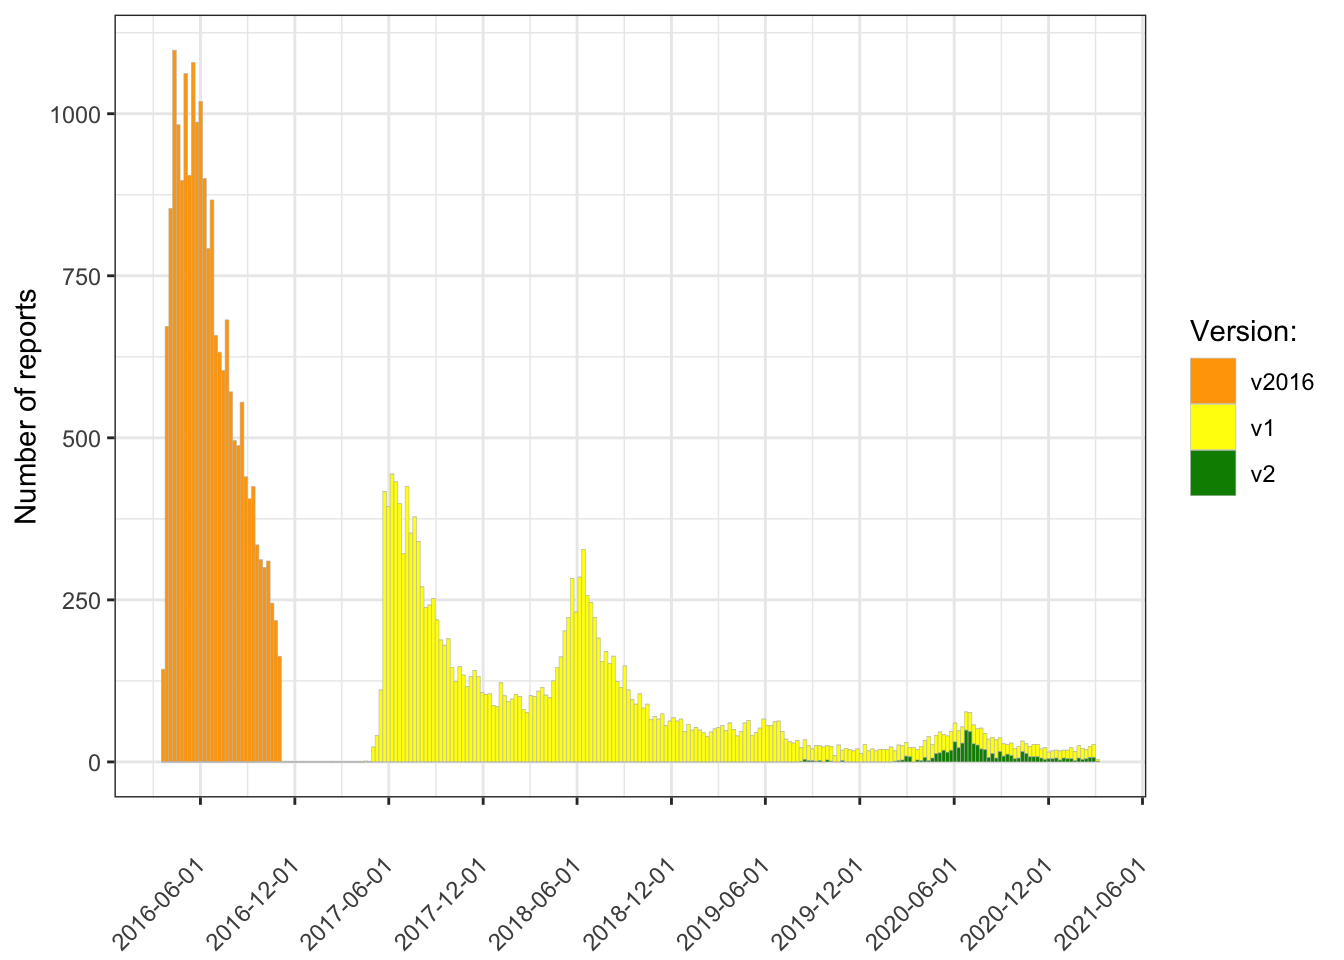
\includegraphics{paper_2_files/figure-latex/unnamed-chunk-1-1.pdf}

\emph{NHS England prescription data:}

As a means of validating the data collected using the Britain Breathing
application, Vigo, et al (2018) look at the correlation between the
median lack of wellness reported on the Britain Breathing application
and the number of antihistamines prescribed by general practitioners,
finding that they are very strongly (r = 0.93) correlated. This data is
openly available from OpenPrescribing.net.

\hypertarget{analytical-approach}{%
\subsection{Analytical approach}\label{analytical-approach}}

\hypertarget{clustering-by-level-of-engagement}{%
\subsubsection{\texorpdfstring{\emph{Clustering by level of
engagement}}{Clustering by level of engagement}}\label{clustering-by-level-of-engagement}}

The way in which engagement is understood and operationalised varies a
lot between scholars and fields (Perski, et al.~2017, Yardley, et
al.~2016). This paper seeks to establish how sensitive the impact of
removing disengaged users is to the way engagement is operationalised.

\emph{Threshold methods}

Jaso, et al (2021) describe a general trend in the EMA/ESM literature to
only include participants with a 70\%--90\% compliance rate,
highlighting that this is often selected by convention and not
empirically determined (2021:3). For example Sun, et al (2020) consider
participants who completed less than 10 assessments to be unengaged, and
excluded them for their analysis.

A more data driven applicationroach is found in a study by Kronkvist and
Engstrom (2020), who split their participants into \emph{abstainers},
who completed zero assessments, \emph{dedicated participants} who
completed a number of assessments one standard deviation or more above
the average number of assessments completed by participants, and
\emph{occasional participants} who did not meet the criteria for the two
previous groups.

\emph{Hidden Markov models}

Druce, et al (2017) argue such approaches overlook the complexity of
patterns of engagement. For example a participant may be strongly
engaged with the application for a week, carefully filling in
assessments every day, before having to cease contributing for various
reasons. Under the approaches described above such contributions would
not be labeled as highly engaged (and potentially excluded from
analysis) for either missing a threshold such as 10 contributions, or
for being below some deviation from the mean number of contributions.

Instead, they propose using first order hidden Markov models\ldots{}

Participants were coded as engaged on a given day if they made at least
one contribution to the application. This variable was assumed to be the
result of participants being in one of three latent states of engagement

\emph{Comparing with prescription data}

Data on antihistamine prescriptions is available from OpenPrescribing at
the Clinical Commissioning Group (\emph{CCG}) level. To enable
comparisons with Britain Breathing data, reports were assigned to the
CCG areas in which they were submitted using the sf package (Pebesma,
2018).

Vigo, et al (2018)\ldots{} \textbf{XXXX I started to write up what had
been done in vigo et al here before outlining what i planned to do, but
it's not actually clear what was done in the original paper XXXX}

\textbf{\textless---- Note: Amount vs Quantity}

\textbf{From the Open prescribe website:}

\textbf{``\emph{Items}~counts the number of times a medicine has been
prescribed. It says nothing about how much of it has been prescribed
(for that see
\href{https://openprescribing.net/faq/\#prescquantity}{quantity}) as
some presciptions will be for many weeks' worth of treatment while
others will be much smaller.}

\textbf{\emph{Quantity}} \textbf{is the total amount of a medicine that
has been prescribed, but the units used depend on the particular form
the medicine is in''}

\textbf{I'm not sure exactly which variable to use here, items would
seem to indicate how often people go to the doctor with Hayfever
problems, quantity is the amount that has been prescribed, which I would
assume is more to do with the gp's personal preferences than the
patients? (my personal experience with hayfever has been to just buy
over the counter loratadine, rather than go through the NHS, which can
take weeks)}

\hfill\break
\textless----

\hypertarget{group-differences}{%
\subsubsection{Group differences}\label{group-differences}}

To asses the impact of removing unengaged participants, this paper
compares the characteristics of respondents from engaged and unengaged
groups.

\emph{Demographics}

Previous studies have explored associations between engagement and
demographic characteristics.

Perski, et al (2017) report age, gender, education, employment and
ethnicity as the most commonly found associations with engagement and
attrition. Similarly, Druce, et al (2017) find that age differs notably
between groups (with engaged participants being over 5 years older on
average), and a substantially lower proportion of women were present in
the ``tourist'' cluster. Kronkvist and Engstrom (2020) find that age and
being female is associated with higher engagement in the study, as do
Rintala, et al (2019). Turner, et al (2017) find that race/ethnicity,
education, and age are are associated with higher levels of engagement.

\textbf{(Would this \^{} be better presented as a table?)}

Britain breathing asks participants for their age and gender which will
allow these characteristics to be compared. Furthermore the geotagged
nature of the reports allows us to determine whether the reports are
made in an urban or rural setting.

\emph{Symptom intensity}

One possible factor in whether or not a participant chooses to
contribute to the application on a given day may be the severity of the
symptoms they are experiencing. Fig x shows that reports peak every year
around pollen season. One possible mechanism is that as symptoms
subside, participants stop reporting.

\begin{verbatim}
## Warning: Transformation introduced infinite values in continuous y-axis
\end{verbatim}

\begin{verbatim}
## Warning: Removed 542 rows containing missing values (geom_bar).
\end{verbatim}

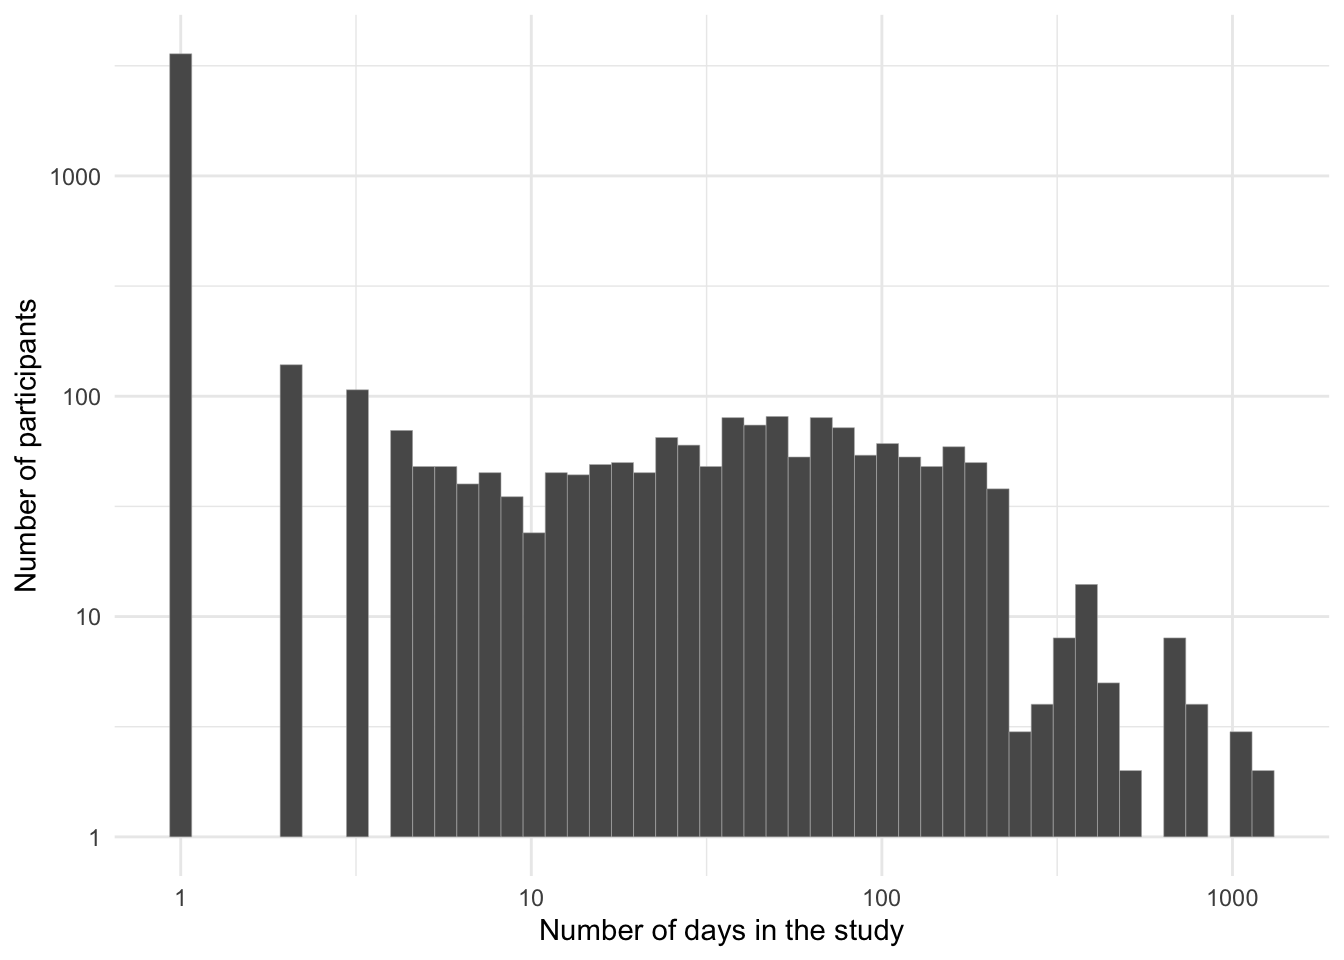
\includegraphics{paper_2_files/figure-latex/unnamed-chunk-2-1.pdf}

\#\#\#\emph{Correlation analysis}

Vigo Vigo, et al (2018) look at the correlation between the median lack
of wellness reported on the Britain Breathing application and the number
of antihistamines prescribed by general practitioners, finding that they
are very strongly (Pearson's r = 0.93) correlated.

Pearson correlation coefficients are calculated between each engagement
cluster and the number of antihistamine prescriptions.

To test whether the correlation observed between the prescription data
and the reported symptom intensity of low-engagement users was
significantly different from the correlation observed between the
prescription data and the reported symptom intensity of high-engagement
users, the Fisher z-transformation (Fisher, 1921) was applied to each
correlation coefficient.

The difference between two z-transformed coefficients approximately
follows a normal distribution with known variance, allowing p-values for
the two-tailed hypothesis test that the difference between observed
correlations is not zero to be calculated (Li, 2019).

\hypertarget{results}{%
\section{Results}\label{results}}

\hypertarget{descriptive-results}{%
\subsection{Descriptive results}\label{descriptive-results}}

\hypertarget{separating-data-into-years}{%
\subsubsection{\texorpdfstring{\emph{Separating data into
years}}{Separating data into years}}\label{separating-data-into-years}}

\begin{figure}
\centering
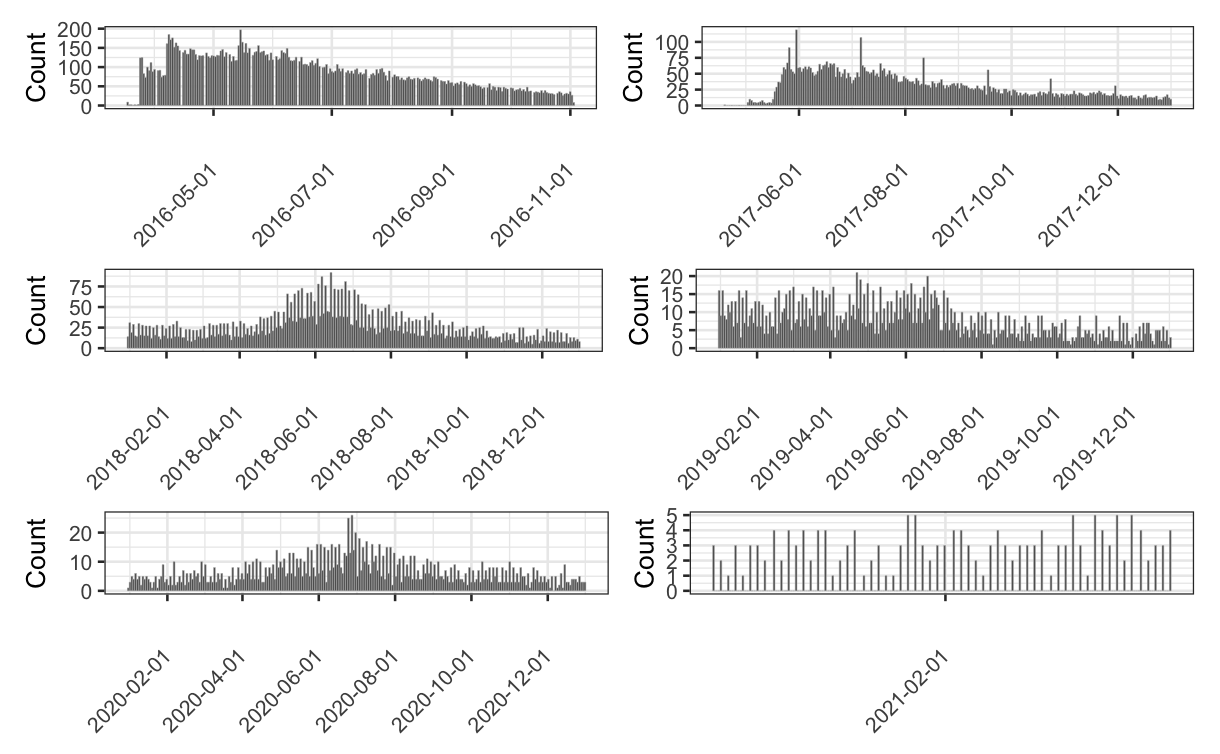
\includegraphics{images/years.png}
\caption{Fig x}
\end{figure}

Britain Breathing data is available from April 2016 to April 2021. There
were 200 982 contributions by 4 748 participants in 2016, 74 183
contributions by 335 participants in 2017, 65 534 contributions by 269
participants in 2018, 19 115 contributions by 78 participants in 2019,
16 446 contributions by 52 participants in 2020, and 182 contributions
by 9 users in 2021.

Data was submitted throughout the year, with the exception of 2017,
where data collection began in May, and in 2021, where data is available
from January until the beginning of March

Data was analysed for each year, with the exception of 2021, due to the
limited amount and temporal coverage of data for that year (fig x).

\hypertarget{participation-inequality}{%
\subsubsection{Participation
inequality}\label{participation-inequality}}

A common feature of citizen science data is high levels of participation
inequality (Hackley, 2016). This feature can also be seen in the Britain
Britain data. A Gini score was calculated for the number of
contributions per participant, finding a value of \textasciitilde0.79
indicating a high level of inequality.

\begin{Shaded}
\begin{Highlighting}[]
\CommentTok{\#Measures of inequality}

\NormalTok{counts }\OtherTok{\textless{}{-}}\NormalTok{ df }\SpecialCharTok{\%\textgreater{}\%}
   \FunctionTok{group\_by}\NormalTok{(user\_id) }\SpecialCharTok{\%\textgreater{}\%}
   \FunctionTok{count}\NormalTok{() }\SpecialCharTok{\%\textgreater{}\%} \FunctionTok{ungroup}\NormalTok{()}

\NormalTok{dineq}\SpecialCharTok{::}\FunctionTok{gini.wtd}\NormalTok{(counts}\SpecialCharTok{$}\NormalTok{n)}

\NormalTok{dineq}\SpecialCharTok{::}\FunctionTok{polar.wtd}\NormalTok{(counts}\SpecialCharTok{$}\NormalTok{n)}

\NormalTok{dineq}\SpecialCharTok{::}\FunctionTok{mld.wtd}\NormalTok{(counts}\SpecialCharTok{$}\NormalTok{n)}
\end{Highlighting}
\end{Shaded}

Fig X shows how many participants have reported on a given number of
days. The log-log scale makes clear that the overwhelmingly most common
behavior was for participants to make a single contribution.

This is in line with findings from (XXXX add Short list of projects
which show single contributions (Jaso and geerharts?, or maybe not just
esm XXXX).

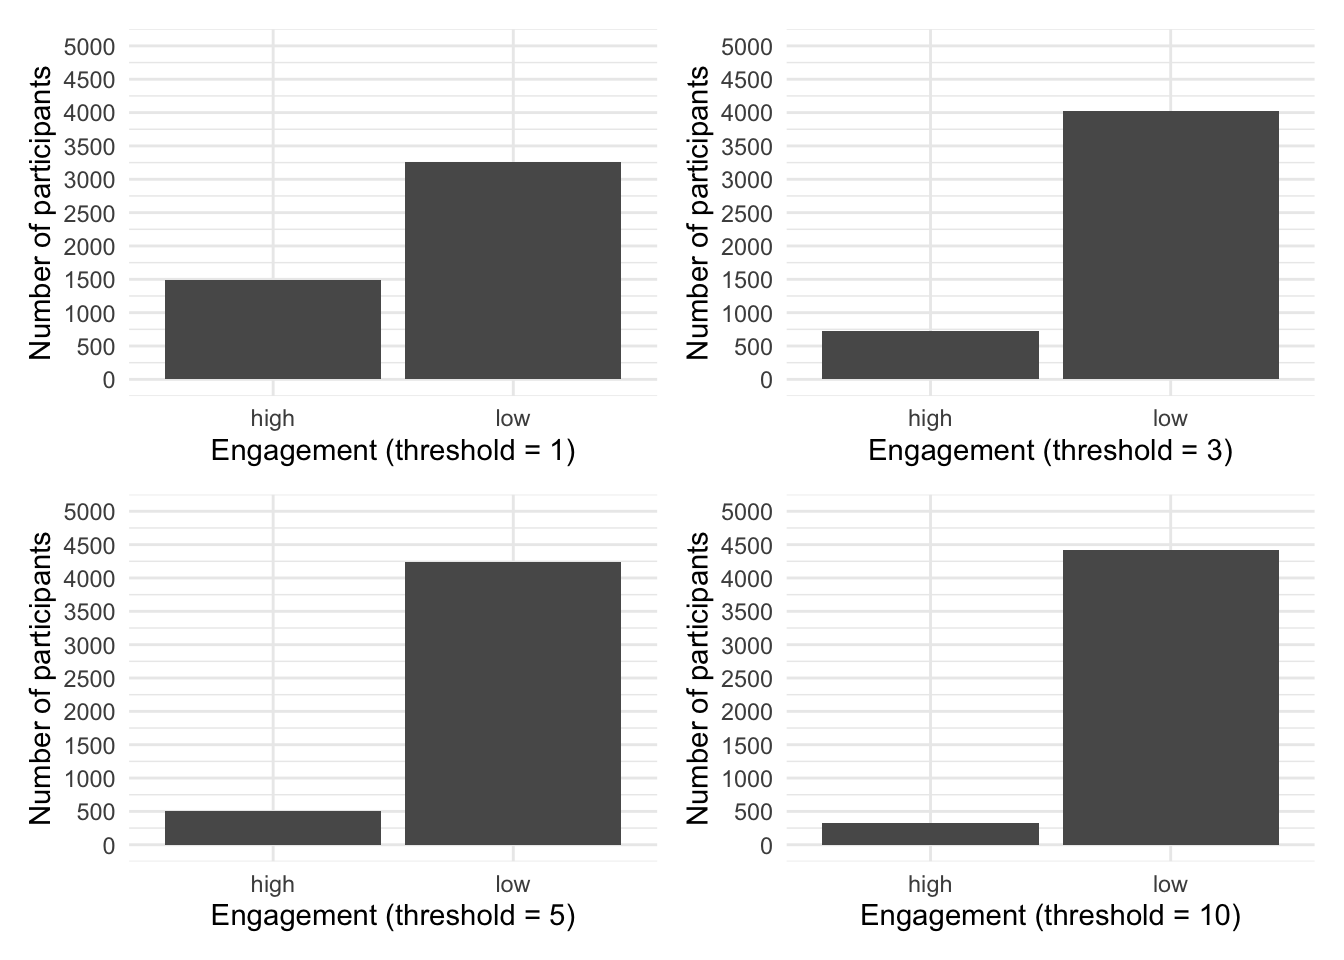
\includegraphics{paper_2_files/figure-latex/unnamed-chunk-4-1.pdf}

\hypertarget{clusterings}{%
\subsubsection{Clusterings}\label{clusterings}}

\emph{Simple clusterings}

The most common way of operationalising engagement is using contribution
thresholds (Jaso, et al.~2021). According to this approach, a
participant is considered to not have engaged with the study if they
contribute less than a certain number of reports. Figure X shows how
participants in the first year would be classified according to this
approach using 4 thresholds: 1, 3, 5, and 10.

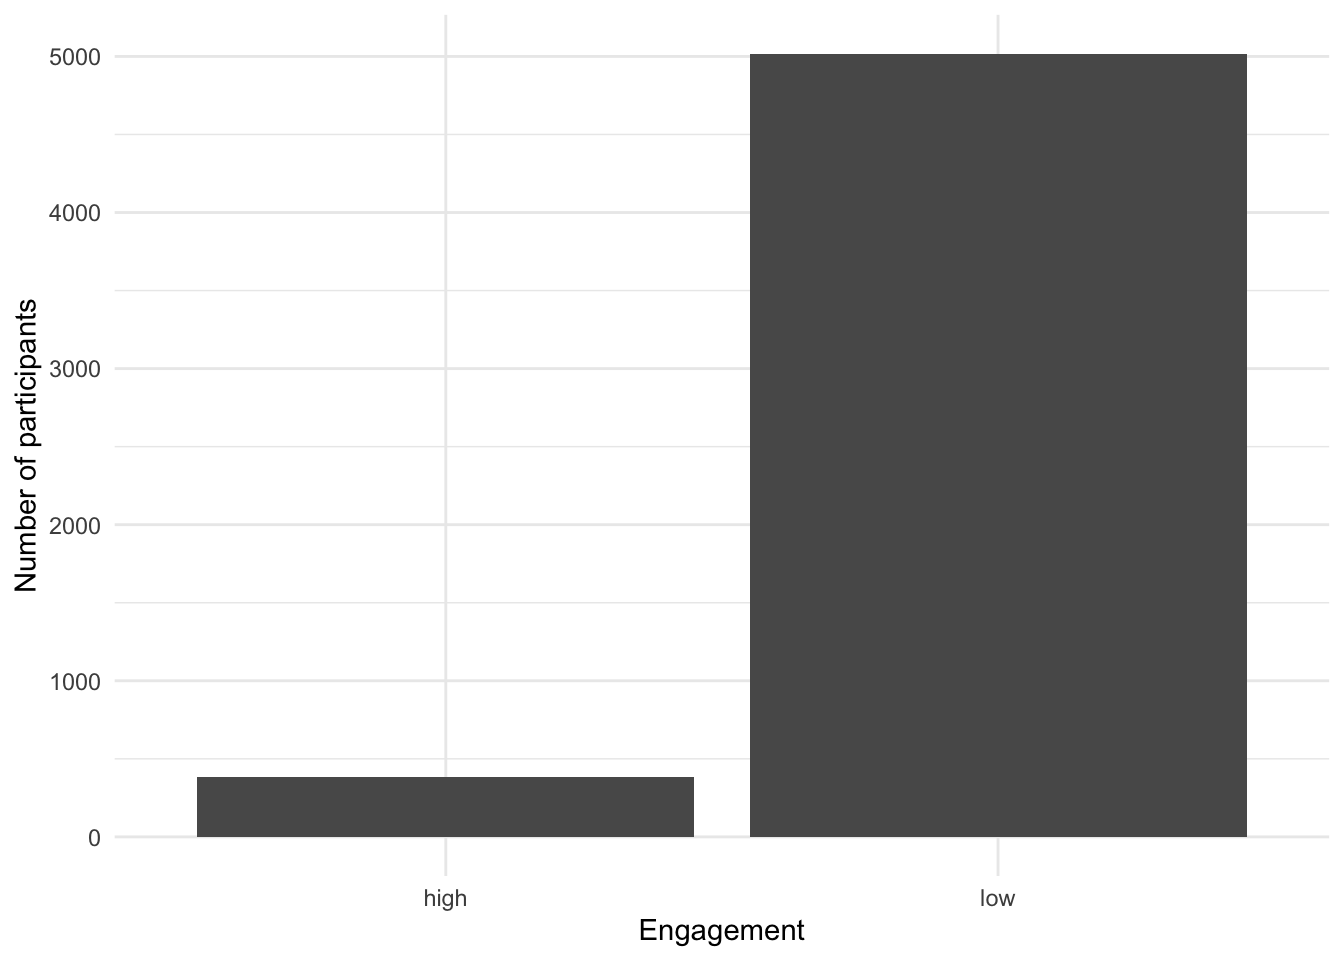
\includegraphics{paper_2_files/figure-latex/unnamed-chunk-6-1.pdf}

Kronkvist and Engstrom (2020) split their participants into abstainers,
who completed zero assessments, dedicated participants who completed a
number of assessments one standard deviation or more above the average
number of assessments completed by participants, and occasional
participants who did not meet the criteria for the two previous groups.
The mean number of contributions by participants in the first year of
the study was \textasciitilde4 and the standard deviation
\textasciitilde{} 13. Figure X shows how participants would be
classified according to this approach.

\includegraphics{paper_2_files/figure-latex/unnamed-chunk-8-1.pdf}

\emph{Hidden Markov Models}

Druce, et al (2017) suggest using hidden Markov models as a better way
of operationalising engagement. This paper applies the approach used in
their paper to the Britain Breathing data.

First dummy variable was created for whether or a participant had made a
contribution on a given day. One limitation of this approach is that
some participants very occasionally made more than one report in a
single day, potentially indicating higher engagement.

Hidden Markov models were then fit on this data using the depmixS4 R
package (Visser, 2021) to estimate the latent level of each participant
on a given day.

The model assumed that whether or not a participant would contribute on
a given day was explained by them being in one of three latent states,
high engagement (with a probability of contributing of 0.7) , low
engagement (with a probability of contributing of 0.1), and disengaged
(with a probability of contributing set at 1e-10, as the software does
not allow for values of zero).

The disengaged state was assumed to be an absorbing state, meaning that
once a participant was in the disengaged state, their probability of
transitioning to another state was zero.

The model also assumed that all participants were in the highly engaged
state on the day they began the study.

Finally participants were clustered according to the history of latent
states inferred by the hidden Markov models using a Markov mixture
model.

\begin{Shaded}
\begin{Highlighting}[]
\CommentTok{\#Loading these manually as they take a long time to run}

\NormalTok{yr1\_k4          }\OtherTok{\textless{}{-}} \FunctionTok{readRDS}\NormalTok{(}\AttributeTok{file =}\NormalTok{ here}\SpecialCharTok{::}\FunctionTok{here}\NormalTok{(}\StringTok{"Clusterings"}\NormalTok{, }\StringTok{"yr1\_k4"}\NormalTok{))}
     
\NormalTok{yr1\_k4\_clusters }\OtherTok{\textless{}{-}} \FunctionTok{readRDS}\NormalTok{(}\AttributeTok{file =}\NormalTok{ here}\SpecialCharTok{::}\FunctionTok{here}\NormalTok{(}\StringTok{"Clusterings"}\NormalTok{, }\StringTok{"yr1\_k4\_clusters"}\NormalTok{ ))}

\NormalTok{yr2\_k4          }\OtherTok{\textless{}{-}} \FunctionTok{readRDS}\NormalTok{(}\AttributeTok{file =}\NormalTok{ here}\SpecialCharTok{::}\FunctionTok{here}\NormalTok{(}\StringTok{"Clusterings"}\NormalTok{, }\StringTok{"yr2\_k4"}\NormalTok{))}
     
\NormalTok{yr2\_k4\_clusters }\OtherTok{\textless{}{-}} \FunctionTok{readRDS}\NormalTok{(}\AttributeTok{file =}\NormalTok{ here}\SpecialCharTok{::}\FunctionTok{here}\NormalTok{(}\StringTok{"Clusterings"}\NormalTok{, }\StringTok{"yr2\_k4\_clusters"}\NormalTok{ )) }

\NormalTok{yr3\_k4          }\OtherTok{\textless{}{-}} \FunctionTok{readRDS}\NormalTok{(}\AttributeTok{file =}\NormalTok{ here}\SpecialCharTok{::}\FunctionTok{here}\NormalTok{(}\StringTok{"Clusterings"}\NormalTok{, }\StringTok{"yr3\_k4"}\NormalTok{))}
     
\NormalTok{yr3\_k4\_clusters }\OtherTok{\textless{}{-}} \FunctionTok{readRDS}\NormalTok{(}\AttributeTok{file =}\NormalTok{ here}\SpecialCharTok{::}\FunctionTok{here}\NormalTok{(}\StringTok{"Clusterings"}\NormalTok{, }\StringTok{"yr3\_k4\_clusters"}\NormalTok{ )) }

\NormalTok{yr4\_k4          }\OtherTok{\textless{}{-}} \FunctionTok{readRDS}\NormalTok{(}\AttributeTok{file =}\NormalTok{ here}\SpecialCharTok{::}\FunctionTok{here}\NormalTok{(}\StringTok{"Clusterings"}\NormalTok{, }\StringTok{"yr4\_k4"}\NormalTok{))}
     
\NormalTok{yr4\_k4\_clusters }\OtherTok{\textless{}{-}} \FunctionTok{readRDS}\NormalTok{(}\AttributeTok{file =}\NormalTok{ here}\SpecialCharTok{::}\FunctionTok{here}\NormalTok{(}\StringTok{"Clusterings"}\NormalTok{, }\StringTok{"yr4\_k4\_clusters"}\NormalTok{ )) }

\NormalTok{yr5\_k4          }\OtherTok{\textless{}{-}} \FunctionTok{readRDS}\NormalTok{(}\AttributeTok{file =}\NormalTok{ here}\SpecialCharTok{::}\FunctionTok{here}\NormalTok{(}\StringTok{"Clusterings"}\NormalTok{, }\StringTok{"yr5\_k4"}\NormalTok{))}
     
\NormalTok{yr5\_k4\_clusters }\OtherTok{\textless{}{-}} \FunctionTok{readRDS}\NormalTok{(}\AttributeTok{file =}\NormalTok{ here}\SpecialCharTok{::}\FunctionTok{here}\NormalTok{(}\StringTok{"Clusterings"}\NormalTok{, }\StringTok{"yr5\_k4\_clusters"}\NormalTok{ )) }
\end{Highlighting}
\end{Shaded}

Using the elbow heuristic for detecting the optimal number of clusters
we find that 4 clusters is optimal.

\textbf{XXXX We don't actually find this at all this time, I found this
the forst time I ran this and it is the most common result (there are
also other reasons, mostly ease of interpretations, and consistency with
the cloudy paper, why this is preferable). Also, things are much more
consistant after the second year, likely a reflection of a smaller about
of latent behaviours groupings given less participants XXXX}

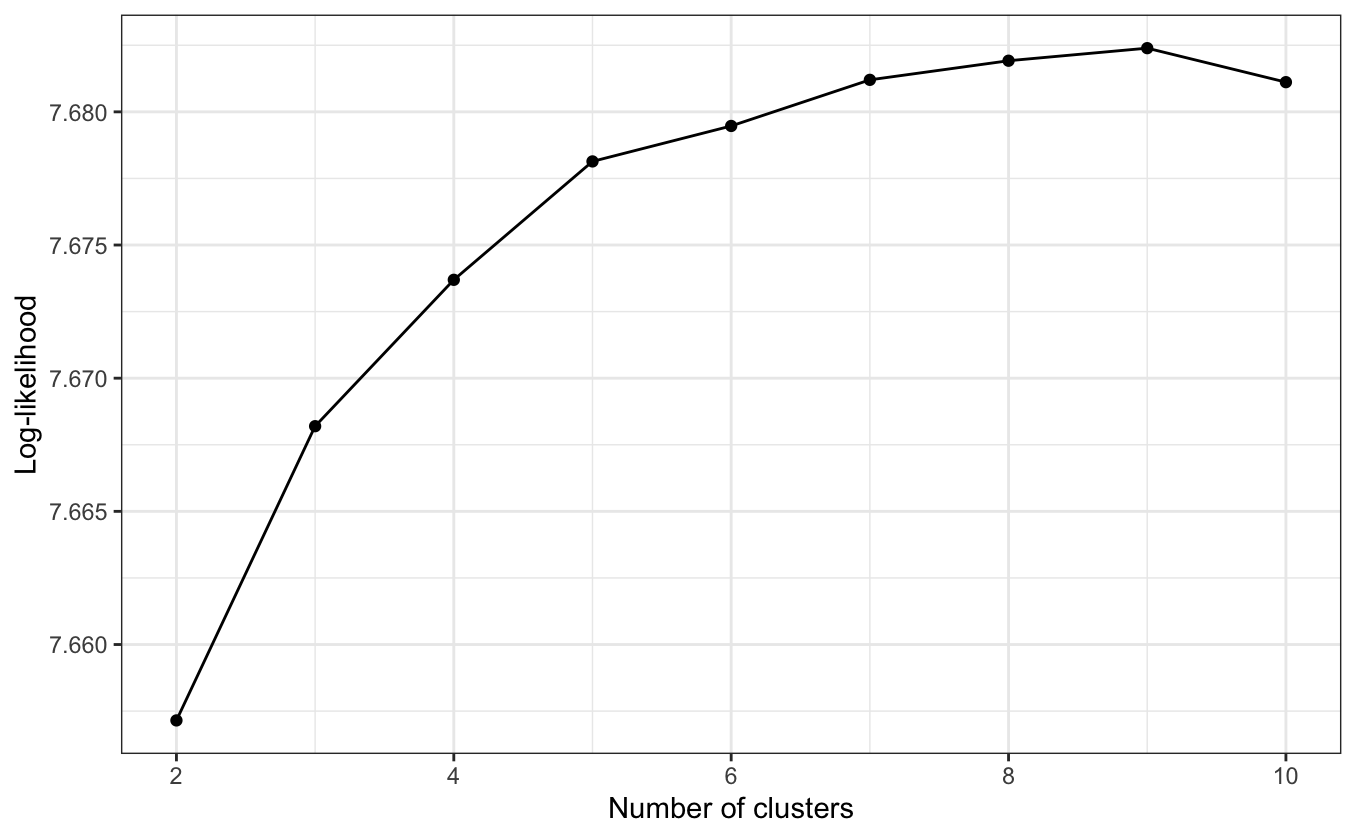
\includegraphics{images/elbow8.png}

\begin{longtable}[]{@{}ll@{}}
\toprule
\endhead
\textbf{Cluster} & \textbf{Number of participants} \\
\textbf{1} & 526 \\
\textbf{2} & 475 \\
\textbf{3} & 3460 \\
\textbf{4} & 287 \\
\bottomrule
\end{longtable}

50 participants were randomly sampled from the study and visualized in
figures x and x. Figure x shows the daily latent state assigned to the
participants by the hidden Markov model, and the cluster assigned to the
participant by the Markov mixture model. Figure x shows days on which
the participant make a contribution, and the final cluster assigned to
the participant by the Markov mixture model. \textbf{(I need to fix the
x axis labels on these)}

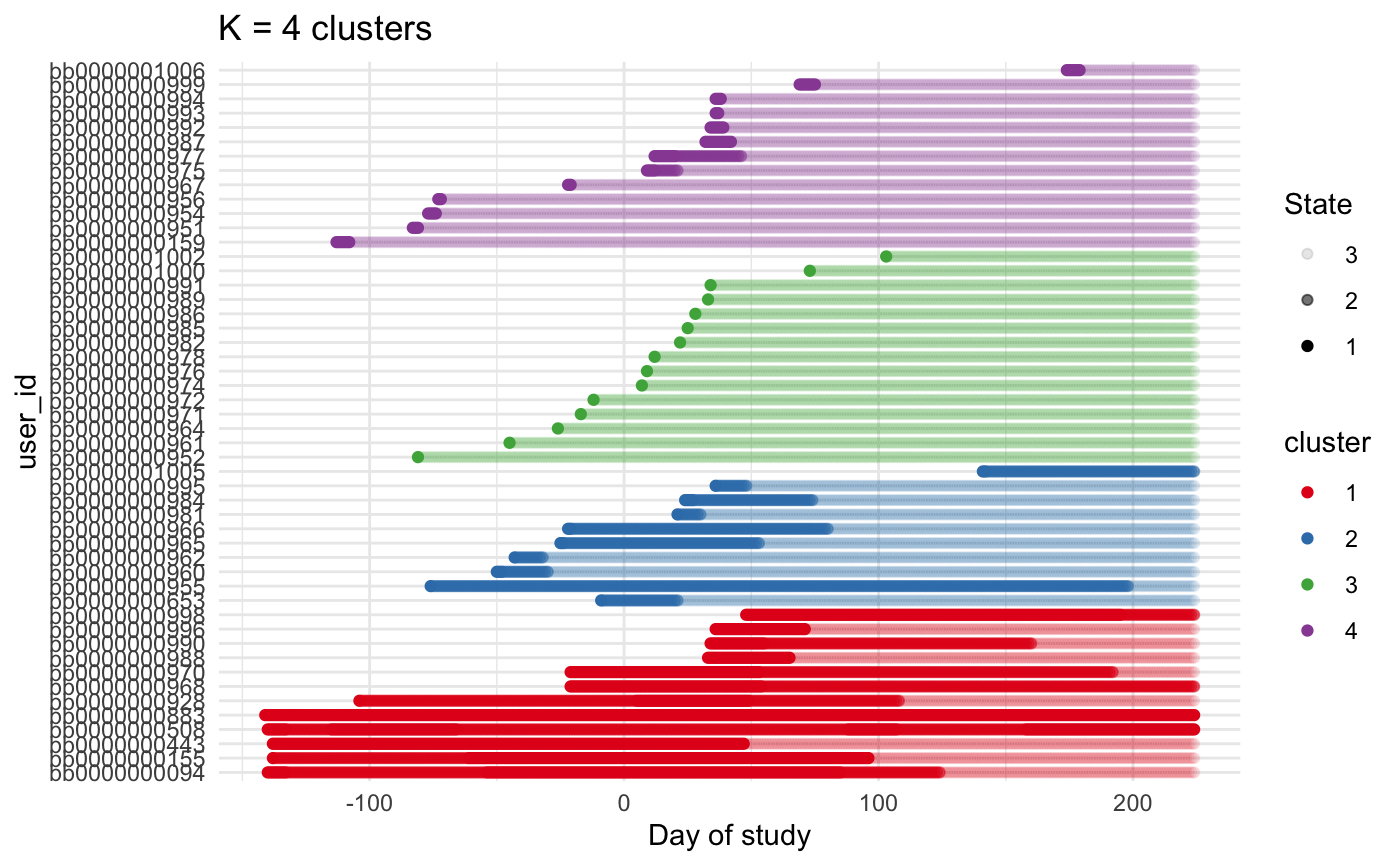
\includegraphics{images/y5.png}

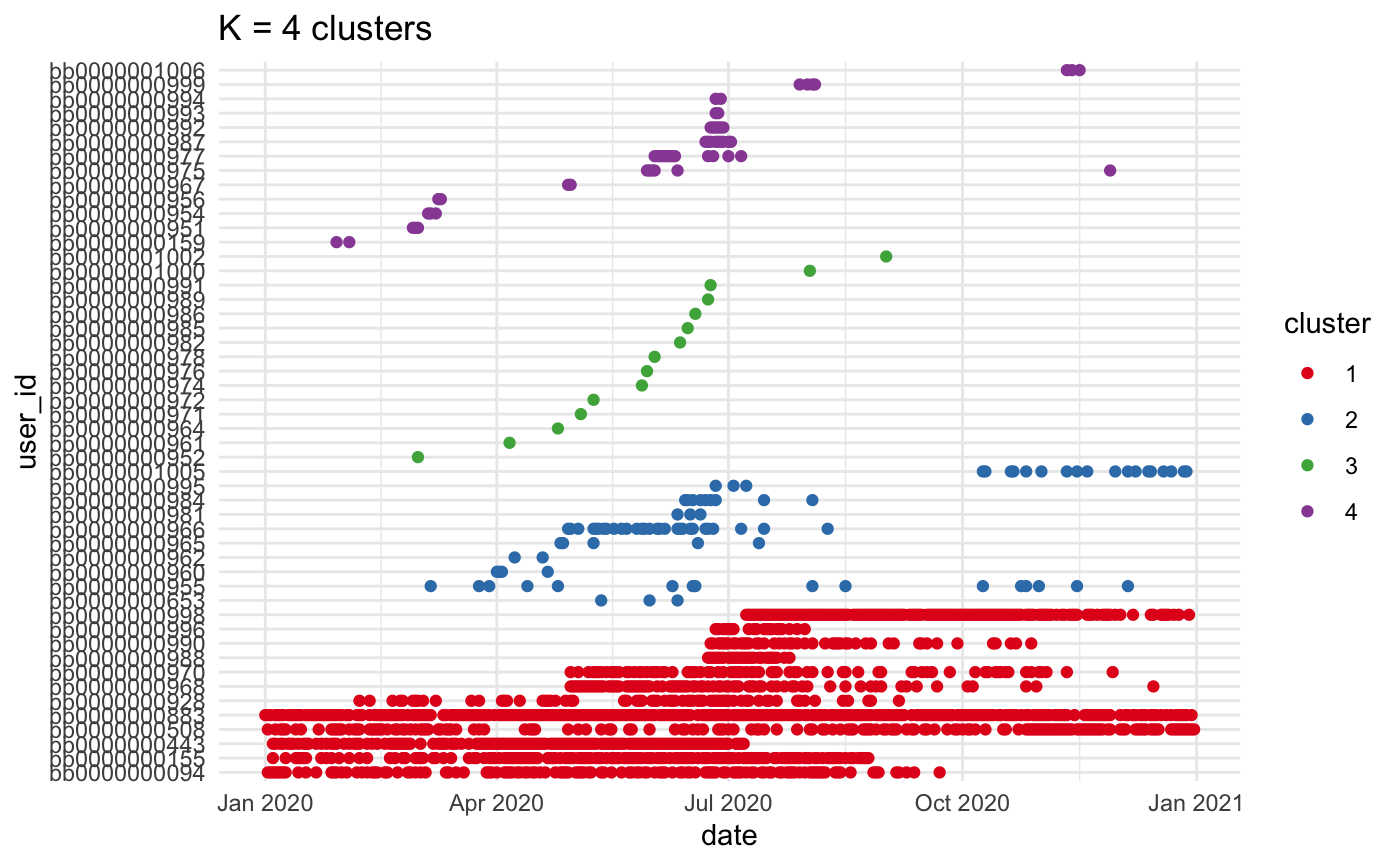
\includegraphics{images/y5b.png}

Visually we can distinguish four reporting behaviors high (cluster 4,
526/4748), medium (cluster 2, 475/4784), low (cluster 4, 278/4784), and
tourist (cluster 1, 3460/4748).

\includegraphics{paper_2_files/figure-latex/unnamed-chunk-10-1.pdf}

\hypertarget{group-differences-1}{%
\subsubsection{Group differences}\label{group-differences-1}}

\emph{Year 1}

\begin{Shaded}
\begin{Highlighting}[]
\NormalTok{y1clust }\OtherTok{\textless{}{-}}\NormalTok{ dfy1 }\SpecialCharTok{\%\textgreater{}\%}
  \FunctionTok{group\_by}\NormalTok{(user\_id) }\SpecialCharTok{\%\textgreater{}\%}
  \FunctionTok{count}\NormalTok{() }\SpecialCharTok{\%\textgreater{}\%}
  \FunctionTok{ungroup}\NormalTok{() }\SpecialCharTok{\%\textgreater{}\%} 
  \FunctionTok{mutate}\NormalTok{(}\AttributeTok{engagement\_threshold\_1 =} \FunctionTok{if\_else}\NormalTok{(n }\SpecialCharTok{\textgreater{}} \DecValTok{1}\NormalTok{, }\StringTok{"high"}\NormalTok{, }\StringTok{"low"}\NormalTok{),}
         \AttributeTok{engagement\_threshold\_3 =} \FunctionTok{if\_else}\NormalTok{(n }\SpecialCharTok{\textgreater{}} \DecValTok{3}\NormalTok{, }\StringTok{"high"}\NormalTok{, }\StringTok{"low"}\NormalTok{),}
         \AttributeTok{engagement\_threshold\_5 =} \FunctionTok{if\_else}\NormalTok{(n }\SpecialCharTok{\textgreater{}} \DecValTok{5}\NormalTok{, }\StringTok{"high"}\NormalTok{, }\StringTok{"low"}\NormalTok{),}
         \AttributeTok{engagement\_threshold\_10 =} \FunctionTok{if\_else}\NormalTok{(n }\SpecialCharTok{\textgreater{}} \DecValTok{10}\NormalTok{, }\StringTok{"high"}\NormalTok{, }\StringTok{"low"}\NormalTok{),}
         \AttributeTok{engagement\_kron =} \FunctionTok{if\_else}\NormalTok{(n }\SpecialCharTok{\textgreater{}} \DecValTok{17}\NormalTok{, }\StringTok{"high"}\NormalTok{, }\StringTok{"low"}\NormalTok{))}\SpecialCharTok{\%\textgreater{}\%} 
  \FunctionTok{left\_join}\NormalTok{(yr1\_k4\_clusters,}\AttributeTok{by =} \StringTok{"user\_id"}\NormalTok{) }\SpecialCharTok{\%\textgreater{}\%} 
\NormalTok{  dplyr}\SpecialCharTok{::}\FunctionTok{select}\NormalTok{(}\SpecialCharTok{{-}}\NormalTok{prob}\FloatTok{.1}\NormalTok{,}
          \SpecialCharTok{{-}}\NormalTok{prob}\FloatTok{.2}\NormalTok{,}
          \SpecialCharTok{{-}}\NormalTok{prob}\FloatTok{.3}\NormalTok{,}
          \SpecialCharTok{{-}}\NormalTok{prob}\FloatTok{.4}\NormalTok{,}
          \SpecialCharTok{{-}}\NormalTok{n) }\SpecialCharTok{\%\textgreater{}\%} 
  \FunctionTok{left\_join}\NormalTok{(dfy1,}\AttributeTok{by =} \StringTok{"user\_id"}\NormalTok{) }\SpecialCharTok{\%\textgreater{}\%} 
  \FunctionTok{mutate}\NormalTok{(}\AttributeTok{age =} \DecValTok{2016}\SpecialCharTok{{-}} \FunctionTok{as.numeric}\NormalTok{(year\_of\_birth))}

\NormalTok{y1clust }\SpecialCharTok{\%\textgreater{}\%}
  \FunctionTok{group\_by}\NormalTok{(cluster) }\SpecialCharTok{\%\textgreater{}\%}
  \FunctionTok{summarise}\NormalTok{(}\AttributeTok{mean\_age =} \FunctionTok{mean}\NormalTok{(age))}

\NormalTok{beh }\OtherTok{\textless{}{-}}\NormalTok{ y1clust }\SpecialCharTok{\%\textgreater{}\%}
  \FunctionTok{group\_by}\NormalTok{(cluster) }\SpecialCharTok{\%\textgreater{}\%}
  \FunctionTok{count}\NormalTok{(gender)}

\NormalTok{beh }\OtherTok{\textless{}{-}}\NormalTok{ y1clust }\SpecialCharTok{\%\textgreater{}\%}
  \FunctionTok{group\_by}\NormalTok{(cluster) }\SpecialCharTok{\%\textgreater{}\%}
  \FunctionTok{count}\NormalTok{()}



\FunctionTok{tribble}\NormalTok{(}
  \SpecialCharTok{\textasciitilde{}}\NormalTok{Cluster, }\SpecialCharTok{\textasciitilde{}}\StringTok{"High engagement"}\NormalTok{, }\SpecialCharTok{\textasciitilde{}}\StringTok{"Medium engagement"}\NormalTok{,}\SpecialCharTok{\textasciitilde{}}\StringTok{"Low engagement"}\NormalTok{,}\SpecialCharTok{\textasciitilde{}}\StringTok{"Tourists"}\NormalTok{,}
  \StringTok{"Female (\%)"}\NormalTok{,   }\DecValTok{1}\NormalTok{,}
  \StringTok{"b"}\NormalTok{,   }\DecValTok{2}\NormalTok{,}
  \StringTok{"c"}\NormalTok{,   }\DecValTok{3}
\NormalTok{)}
\end{Highlighting}
\end{Shaded}

\emph{Year 2}

\emph{Year 3}

\emph{Year 4}

\emph{Year 5}

\hypertarget{gender}{%
\paragraph{Gender}\label{gender}}

Pearson's Chi squared test was used to test for differences in gender
between high and low engagement clusters. The strength of the
association was measured using Cramer's V (Cramér, 1946). Cramer's V is
bounded between zero and one, with zero indicating no association, and
one indicating a perfect association.

\emph{Threshold approaches}

\begin{longtable}[]{@{}rrrrlr@{}}
\toprule
Year & Threshold & \% Female (high) & \% Female (low) & p & Cramer's
V \\
\midrule
\endhead
1 & 1 & 52 & 47 & \textasciitilde0.00 & 0.040 \\
1 & 3 & 53 & 47 & \textasciitilde0.00 & 0.050 \\
1 & 5 & 53 & 49 & \textasciitilde0.00 & 0.030 \\
1 & 10 & 53 & 49 & \textasciitilde0.00 & 0.030 \\
2 & 1 & 55 & 58 & \textasciitilde0.6 & 0.000 \\
2 & 3 & 55 & 54 & \textasciitilde{} 0.94 & 0.000 \\
2 & 5 & 55 & 53 & \textasciitilde0.62 & 0.000 \\
2 & 10 & 54 & 57 & \textasciitilde0.28 & 0.005 \\
3 & 1 & 45 & 64 & \textasciitilde0.00 & 0.040 \\
3 & 3 & 44 & 65 & \textasciitilde0.00 & 0.070 \\
3 & 5 & 44 & 66 & \textasciitilde0.00 & 0.090 \\
3 & 10 & 44 & 59 & \textasciitilde0.00 & 0.070 \\
4 & 1 & 23 & 73 & \textasciitilde0.00 & 0.120 \\
4 & 3 & 22 & 82 & \textasciitilde0.00 & 0.260 \\
4 & 5 & 21 & 77 & \textasciitilde0.00 & 0.300 \\
4 & 10 & 20 & 70 & \textasciitilde0.00 & 0.300 \\
5 & 1 & 19 & 50 & \textasciitilde0.00 & 0.070 \\
5 & 3 & 18 & 61 & \textasciitilde0.00 & 0.170 \\
5 & 5 & 18 & 58 & \textasciitilde0.00 & 0.190 \\
5 & 10 & 17 & 65 & \textasciitilde0.00 & 0.280 \\
\bottomrule
\end{longtable}

In the first year, the proportion of reports made by women was always
higher in the high engagement groups compared to low engagement groups,
regardless of the threshold chosen. The associations were very small but
significant.

In the second year, the proportion of reports made by women was higher
in the high engagement groups only when using thresholds of 3 and 5. The
associations were very small and were not statistically significant.

In the third year, the proportion of reports made by women was always
higher in the low engagement groups compared to high engagement groups,
regardless of the threshold chosen. The associations were small and
significant.

In the fourth year, the proportion of reports made by women was always
higher in the low engagement groups compared to high engagement groups,
regardless of the threshold chosen. The associations were moderate and
significant.

In the fifth year, the proportion of reports made by women was always
higher in the low engagement groups compared to high engagement groups,
regardless of the threshold chosen. The associations were moderate and
significant.

\hypertarget{urban}{%
\paragraph{Urban}\label{urban}}

\emph{Threshold approaches}

\begin{longtable}[]{@{}rrrrlr@{}}
\toprule
Year & Threshold & \% Rural (high) & \% Rural (low) & p & Cramer's V \\
\midrule
\endhead
1 & 1 & 20 & 19 & 0.65 & 0.00 \\
1 & 3 & 19 & 20 & 0.70 & 0.00 \\
1 & 5 & 19 & 20 & 0.30 & 0.00 \\
1 & 10 & 19 & 21 & \textasciitilde0.00 & 0.02 \\
2 & 1 & 24 & 20 & 0.39 & 0.00 \\
2 & 3 & 24 & 15 & \textasciitilde0.00 & 0.03 \\
2 & 5 & 24 & 16 & \textasciitilde0.00 & 0.04 \\
2 & 10 & 25 & 18 & \textasciitilde0.00 & 0.04 \\
3 & 1 & 29 & 27 & 0.57 & 0.00 \\
3 & 3 & 30 & 23 & 0.07 & 0.02 \\
3 & 5 & 30 & 26 & 0.16 & 0.01 \\
3 & 10 & 30 & 26 & 0.08 & 0.02 \\
4 & 1 & 36 & 23 & 0.21 & 0.02 \\
4 & 3 & 36 & 19 & \textasciitilde0.00 & 0.06 \\
4 & 5 & 36 & 22 & \textasciitilde0.00 & 0.06 \\
4 & 10 & 37 & 16 & \textasciitilde0.00 & 0.11 \\
5 & 1 & 26 & 12 & 0.22 & 0.02 \\
5 & 3 & 26 & 11 & 0.03 & 0.05 \\
5 & 5 & 26 & 8 & \textasciitilde0.00 & 0.08 \\
5 & 10 & 26 & 14 & \textasciitilde0.01 & 0.06 \\
\bottomrule
\end{longtable}

\hypertarget{correlation-analysis}{%
\subsubsection{Correlation analysis}\label{correlation-analysis}}

NHS prescription data is available from OpenPrescribing.net. However
this data is only available for prescriptions made in England. Reports
made outside of England (1697, or \textasciitilde8.4\% of reports) were
therefore removed from the data, as they could not be linked to
prescription data.

With all data included, the Pearson coefficient for the correlation
between symptom intensity and the number of prescribed items was 0.68
for year one, 0.79 for year two, 0.93 for year three, 0.52 for year
four, and 0.21 for year five.

\emph{Threshold approaches}

\emph{Year 1}

For a threshold of 1, the correlation with low-engagement reports was
\textasciitilde0.51, the correlation with high-engagement reports was
\textasciitilde0.71. The difference is not statistically significant
with a p-value of \textasciitilde0.43.

For a threshold of 3, the correlation with low-engagement reports was
\textasciitilde0.55, the correlation with low-engagement reports was
\textasciitilde0.76. The difference is not statistically significant
with a p-value of \textasciitilde0.36.

For a threshold of 5, the correlation with low-engagement reports was
\textasciitilde0.53, the correlation with high-engagement reports was
\textasciitilde0.76. The difference is not statistically significant
with a p-value of \textasciitilde0.32.

For a threshold of 10, the correlation with low-engagement reports was
\textasciitilde0.56, the correlation with high-engagement reports was
\textasciitilde0.81. The difference is not statistically significant
with a p-value of \textasciitilde0.22.

\begin{Shaded}
\begin{Highlighting}[]
\NormalTok{ letest }\OtherTok{\textless{}{-}}\NormalTok{  dfy1 }\SpecialCharTok{\%\textgreater{}\%}
   \FunctionTok{group\_by}\NormalTok{(user\_id) }\SpecialCharTok{\%\textgreater{}\%}
   \FunctionTok{count}\NormalTok{() }\SpecialCharTok{\%\textgreater{}\%}
   \FunctionTok{ungroup}\NormalTok{() }\SpecialCharTok{\%\textgreater{}\%} 
   \FunctionTok{mutate}\NormalTok{(}\AttributeTok{engagement\_threshold\_1 =} \FunctionTok{if\_else}\NormalTok{(n }\SpecialCharTok{\textgreater{}} \DecValTok{1}\NormalTok{, }\StringTok{"high"}\NormalTok{, }\StringTok{"low"}\NormalTok{),}
          \AttributeTok{engagement\_threshold\_3 =} \FunctionTok{if\_else}\NormalTok{(n }\SpecialCharTok{\textgreater{}} \DecValTok{3}\NormalTok{, }\StringTok{"high"}\NormalTok{, }\StringTok{"low"}\NormalTok{),}
          \AttributeTok{engagement\_threshold\_5 =} \FunctionTok{if\_else}\NormalTok{(n }\SpecialCharTok{\textgreater{}} \DecValTok{5}\NormalTok{, }\StringTok{"high"}\NormalTok{, }\StringTok{"low"}\NormalTok{),}
          \AttributeTok{engagement\_threshold\_10 =} \FunctionTok{if\_else}\NormalTok{(n }\SpecialCharTok{\textgreater{}} \DecValTok{10}\NormalTok{, }\StringTok{"high"}\NormalTok{, }\StringTok{"low"}\NormalTok{),}
          \AttributeTok{engagement\_kron =} \FunctionTok{if\_else}\NormalTok{(n }\SpecialCharTok{\textgreater{}} \DecValTok{17}\NormalTok{, }\StringTok{"high"}\NormalTok{, }\StringTok{"low"}\NormalTok{)) }\SpecialCharTok{\%\textgreater{}\%} 
   \FunctionTok{left\_join}\NormalTok{(yr1\_k4\_clusters,}\AttributeTok{by =} \StringTok{"user\_id"}\NormalTok{) }\SpecialCharTok{\%\textgreater{}\%} 
\NormalTok{   dplyr}\SpecialCharTok{::}\FunctionTok{select}\NormalTok{(}\SpecialCharTok{{-}}\NormalTok{prob}\FloatTok{.1}\NormalTok{,}
                 \SpecialCharTok{{-}}\NormalTok{prob}\FloatTok{.2}\NormalTok{,}
                 \SpecialCharTok{{-}}\NormalTok{prob}\FloatTok{.3}\NormalTok{,}
                 \SpecialCharTok{{-}}\NormalTok{prob}\FloatTok{.4}\NormalTok{,}
                 \SpecialCharTok{{-}}\NormalTok{n) }\SpecialCharTok{\%\textgreater{}\%} 
  \FunctionTok{filter}\NormalTok{(engagement\_threshold\_5 }\SpecialCharTok{==} \StringTok{"high"}\NormalTok{) }\SpecialCharTok{\%\textgreater{}\%}
   \FunctionTok{left\_join}\NormalTok{(dfy1,}\AttributeTok{by =} \StringTok{"user\_id"}\NormalTok{) }\SpecialCharTok{\%\textgreater{}\%}  
   \FunctionTok{group\_by}\NormalTok{(lubridate}\SpecialCharTok{::}\FunctionTok{month}\NormalTok{(date)) }\SpecialCharTok{\%\textgreater{}\%}
   \FunctionTok{summarise}\NormalTok{(}\AttributeTok{reports =} \FunctionTok{n}\NormalTok{(),}
             \AttributeTok{mean\_how =} \FunctionTok{mean}\NormalTok{(how\_im\_doing),}
             \AttributeTok{median\_how =} \FunctionTok{median}\NormalTok{(how\_im\_doing)) }\SpecialCharTok{\%\textgreater{}\%}
   \FunctionTok{left\_join}\NormalTok{(presc\_vigo, }\AttributeTok{by =} \FunctionTok{c}\NormalTok{( }\StringTok{"lubridate::month(date)"} \OtherTok{=} \StringTok{"month"}\NormalTok{ )) }\SpecialCharTok{\%\textgreater{}\%} 
   \FunctionTok{drop\_na}\NormalTok{(mean\_how) }



\NormalTok{ letest2 }\OtherTok{\textless{}{-}}\NormalTok{ dfy1 }\SpecialCharTok{\%\textgreater{}\%}
   \FunctionTok{group\_by}\NormalTok{(user\_id) }\SpecialCharTok{\%\textgreater{}\%}
   \FunctionTok{count}\NormalTok{() }\SpecialCharTok{\%\textgreater{}\%}
   \FunctionTok{ungroup}\NormalTok{() }\SpecialCharTok{\%\textgreater{}\%} 
   \FunctionTok{mutate}\NormalTok{(}\AttributeTok{engagement\_threshold\_1 =} \FunctionTok{if\_else}\NormalTok{(n }\SpecialCharTok{\textgreater{}} \DecValTok{1}\NormalTok{, }\StringTok{"high"}\NormalTok{, }\StringTok{"low"}\NormalTok{),}
          \AttributeTok{engagement\_threshold\_3 =} \FunctionTok{if\_else}\NormalTok{(n }\SpecialCharTok{\textgreater{}} \DecValTok{3}\NormalTok{, }\StringTok{"high"}\NormalTok{, }\StringTok{"low"}\NormalTok{),}
          \AttributeTok{engagement\_threshold\_5 =} \FunctionTok{if\_else}\NormalTok{(n }\SpecialCharTok{\textgreater{}} \DecValTok{5}\NormalTok{, }\StringTok{"high"}\NormalTok{, }\StringTok{"low"}\NormalTok{),}
          \AttributeTok{engagement\_threshold\_10 =} \FunctionTok{if\_else}\NormalTok{(n }\SpecialCharTok{\textgreater{}} \DecValTok{10}\NormalTok{, }\StringTok{"high"}\NormalTok{, }\StringTok{"low"}\NormalTok{),}
          \AttributeTok{engagement\_kron =} \FunctionTok{if\_else}\NormalTok{(n }\SpecialCharTok{\textgreater{}} \DecValTok{17}\NormalTok{, }\StringTok{"high"}\NormalTok{, }\StringTok{"low"}\NormalTok{)) }\SpecialCharTok{\%\textgreater{}\%} 
   \FunctionTok{left\_join}\NormalTok{(yr1\_k4\_clusters,}\AttributeTok{by =} \StringTok{"user\_id"}\NormalTok{) }\SpecialCharTok{\%\textgreater{}\%} 
\NormalTok{   dplyr}\SpecialCharTok{::}\FunctionTok{select}\NormalTok{(}\SpecialCharTok{{-}}\NormalTok{prob}\FloatTok{.1}\NormalTok{,}
                 \SpecialCharTok{{-}}\NormalTok{prob}\FloatTok{.2}\NormalTok{,}
                 \SpecialCharTok{{-}}\NormalTok{prob}\FloatTok{.3}\NormalTok{,}
                 \SpecialCharTok{{-}}\NormalTok{prob}\FloatTok{.4}\NormalTok{,}
                 \SpecialCharTok{{-}}\NormalTok{n) }\SpecialCharTok{\%\textgreater{}\%} 
  \FunctionTok{filter}\NormalTok{(engagement\_threshold\_5 }\SpecialCharTok{==} \StringTok{"low"}\NormalTok{) }\SpecialCharTok{\%\textgreater{}\%}
   \FunctionTok{left\_join}\NormalTok{(dfy1,}\AttributeTok{by =} \StringTok{"user\_id"}\NormalTok{) }\SpecialCharTok{\%\textgreater{}\%}  
   \FunctionTok{group\_by}\NormalTok{(lubridate}\SpecialCharTok{::}\FunctionTok{month}\NormalTok{(date)) }\SpecialCharTok{\%\textgreater{}\%}
   \FunctionTok{summarise}\NormalTok{(}\AttributeTok{reports =} \FunctionTok{n}\NormalTok{(),}
             \AttributeTok{mean\_how2 =} \FunctionTok{mean}\NormalTok{(how\_im\_doing),}
             \AttributeTok{median\_how =} \FunctionTok{median}\NormalTok{(how\_im\_doing)) }\SpecialCharTok{\%\textgreater{}\%}
   \FunctionTok{left\_join}\NormalTok{(presc\_vigo, }\AttributeTok{by =} \FunctionTok{c}\NormalTok{( }\StringTok{"lubridate::month(date)"} \OtherTok{=} \StringTok{"month"}\NormalTok{ )) }\SpecialCharTok{\%\textgreater{}\%} 
   \FunctionTok{drop\_na}\NormalTok{(mean\_how2)  }
 

   
\NormalTok{ combined }\OtherTok{\textless{}{-}}\NormalTok{ letest2 }\SpecialCharTok{\%\textgreater{}\%} \FunctionTok{select}\NormalTok{(}\StringTok{\textasciigrave{}}\AttributeTok{lubridate::month(date)}\StringTok{\textasciigrave{}}\NormalTok{,}
\NormalTok{                             mean\_how2) }\SpecialCharTok{\%\textgreater{}\%} 
   \FunctionTok{left\_join}\NormalTok{(letest)}
 
\FunctionTok{cor}\NormalTok{(combined}\SpecialCharTok{$}\NormalTok{items, combined}\SpecialCharTok{$}\NormalTok{mean\_how, }\AttributeTok{method=} \StringTok{"pearson"}\NormalTok{)}

\FunctionTok{cor}\NormalTok{(combined}\SpecialCharTok{$}\NormalTok{items, combined}\SpecialCharTok{$}\NormalTok{mean\_how2, }\AttributeTok{method=} \StringTok{"pearson"}\NormalTok{) }
 
\FunctionTok{cor\_significance\_test}\NormalTok{(combined}\SpecialCharTok{$}\NormalTok{items, combined}\SpecialCharTok{$}\NormalTok{mean\_how, combined}\SpecialCharTok{$}\NormalTok{mean\_how2, }\AttributeTok{method=}\StringTok{"pearson"}\NormalTok{)}
\end{Highlighting}
\end{Shaded}

\emph{Year 2}

For a threshold of 1, the correlation with high-engagement reports was
\textasciitilde0.92, the correlation with low-engagement reports was
\textasciitilde0.85. The difference is not statistically significant
with a p-value of \textasciitilde0.47.

For a threshold of 3, the correlation with high-engagement reports was
\textasciitilde0.92, the correlation with low-engagement reports was
\textasciitilde0.75. The difference is not statistically significant
with a p-value of \textasciitilde0.16.

For a threshold of 5, the correlation with high-engagement reports was
\textasciitilde0.92, the correlation with low-engagement reports was
\textasciitilde0.74. The difference is not statistically significant
with a p-value of \textasciitilde0.16.

For a threshold of 10, the correlation with high-engagement reports was
\textasciitilde0.91, the correlation with low-engagement reports was
\textasciitilde0.84. The difference is not statistically significant
with a p-value of \textasciitilde0.49.

\begin{Shaded}
\begin{Highlighting}[]
\NormalTok{ presc\_y2 }\OtherTok{\textless{}{-}}\NormalTok{ presc }\SpecialCharTok{\%\textgreater{}\%} 
   \FunctionTok{filter}\NormalTok{(lubridate}\SpecialCharTok{::}\FunctionTok{year}\NormalTok{(date) }\SpecialCharTok{==} \DecValTok{2017}\NormalTok{) }\SpecialCharTok{\%\textgreater{}\%}
   \FunctionTok{mutate}\NormalTok{(}\AttributeTok{month =}\NormalTok{ lubridate}\SpecialCharTok{::}\FunctionTok{month}\NormalTok{(date)) }\SpecialCharTok{\%\textgreater{}\%} 
   \FunctionTok{group\_by}\NormalTok{(month) }\SpecialCharTok{\%\textgreater{}\%} 
   \FunctionTok{summarise}\NormalTok{(}\AttributeTok{sum =} \FunctionTok{sum}\NormalTok{(items))}


\NormalTok{ letest }\OtherTok{\textless{}{-}}\NormalTok{  dfy2 }\SpecialCharTok{\%\textgreater{}\%}
   \FunctionTok{group\_by}\NormalTok{(user\_id) }\SpecialCharTok{\%\textgreater{}\%}
   \FunctionTok{count}\NormalTok{() }\SpecialCharTok{\%\textgreater{}\%}
   \FunctionTok{ungroup}\NormalTok{() }\SpecialCharTok{\%\textgreater{}\%} 
   \FunctionTok{mutate}\NormalTok{(}\AttributeTok{engagement\_threshold\_1 =} \FunctionTok{if\_else}\NormalTok{(n }\SpecialCharTok{\textgreater{}} \DecValTok{1}\NormalTok{, }\StringTok{"high"}\NormalTok{, }\StringTok{"low"}\NormalTok{),}
          \AttributeTok{engagement\_threshold\_3 =} \FunctionTok{if\_else}\NormalTok{(n }\SpecialCharTok{\textgreater{}} \DecValTok{3}\NormalTok{, }\StringTok{"high"}\NormalTok{, }\StringTok{"low"}\NormalTok{),}
          \AttributeTok{engagement\_threshold\_5 =} \FunctionTok{if\_else}\NormalTok{(n }\SpecialCharTok{\textgreater{}} \DecValTok{5}\NormalTok{, }\StringTok{"high"}\NormalTok{, }\StringTok{"low"}\NormalTok{),}
          \AttributeTok{engagement\_threshold\_10 =} \FunctionTok{if\_else}\NormalTok{(n }\SpecialCharTok{\textgreater{}} \DecValTok{10}\NormalTok{, }\StringTok{"high"}\NormalTok{, }\StringTok{"low"}\NormalTok{),}
          \AttributeTok{engagement\_kron =} \FunctionTok{if\_else}\NormalTok{(n }\SpecialCharTok{\textgreater{}} \DecValTok{17}\NormalTok{, }\StringTok{"high"}\NormalTok{, }\StringTok{"low"}\NormalTok{)) }\SpecialCharTok{\%\textgreater{}\%} 
   \FunctionTok{left\_join}\NormalTok{(yr2\_k4\_clusters,}\AttributeTok{by =} \StringTok{"user\_id"}\NormalTok{) }\SpecialCharTok{\%\textgreater{}\%} 
\NormalTok{   dplyr}\SpecialCharTok{::}\FunctionTok{select}\NormalTok{(}\SpecialCharTok{{-}}\NormalTok{prob}\FloatTok{.1}\NormalTok{,}
                 \SpecialCharTok{{-}}\NormalTok{prob}\FloatTok{.2}\NormalTok{,}
                 \SpecialCharTok{{-}}\NormalTok{prob}\FloatTok{.3}\NormalTok{,}
                 \SpecialCharTok{{-}}\NormalTok{prob}\FloatTok{.4}\NormalTok{,}
                 \SpecialCharTok{{-}}\NormalTok{n) }\SpecialCharTok{\%\textgreater{}\%} 
  \FunctionTok{filter}\NormalTok{(engagement\_threshold\_10 }\SpecialCharTok{==} \StringTok{"high"}\NormalTok{) }\SpecialCharTok{\%\textgreater{}\%}
   \FunctionTok{left\_join}\NormalTok{(dfy2,}\AttributeTok{by =} \StringTok{"user\_id"}\NormalTok{) }\SpecialCharTok{\%\textgreater{}\%}  
   \FunctionTok{group\_by}\NormalTok{(lubridate}\SpecialCharTok{::}\FunctionTok{month}\NormalTok{(date)) }\SpecialCharTok{\%\textgreater{}\%}
   \FunctionTok{summarise}\NormalTok{(}\AttributeTok{reports =} \FunctionTok{n}\NormalTok{(),}
             \AttributeTok{mean\_how =} \FunctionTok{mean}\NormalTok{(nose),}
             \AttributeTok{median\_how =} \FunctionTok{median}\NormalTok{(nose)) }\SpecialCharTok{\%\textgreater{}\%}
   \FunctionTok{left\_join}\NormalTok{(presc\_y2, }\AttributeTok{by =} \FunctionTok{c}\NormalTok{( }\StringTok{"lubridate::month(date)"} \OtherTok{=} \StringTok{"month"}\NormalTok{ )) }\SpecialCharTok{\%\textgreater{}\%} 
   \FunctionTok{drop\_na}\NormalTok{(mean\_how) }



\NormalTok{ letest2 }\OtherTok{\textless{}{-}}\NormalTok{ dfy2 }\SpecialCharTok{\%\textgreater{}\%}
   \FunctionTok{group\_by}\NormalTok{(user\_id) }\SpecialCharTok{\%\textgreater{}\%}
   \FunctionTok{count}\NormalTok{() }\SpecialCharTok{\%\textgreater{}\%}
   \FunctionTok{ungroup}\NormalTok{() }\SpecialCharTok{\%\textgreater{}\%} 
   \FunctionTok{mutate}\NormalTok{(}\AttributeTok{engagement\_threshold\_1 =} \FunctionTok{if\_else}\NormalTok{(n }\SpecialCharTok{\textgreater{}} \DecValTok{1}\NormalTok{, }\StringTok{"high"}\NormalTok{, }\StringTok{"low"}\NormalTok{),}
          \AttributeTok{engagement\_threshold\_3 =} \FunctionTok{if\_else}\NormalTok{(n }\SpecialCharTok{\textgreater{}} \DecValTok{3}\NormalTok{, }\StringTok{"high"}\NormalTok{, }\StringTok{"low"}\NormalTok{),}
          \AttributeTok{engagement\_threshold\_5 =} \FunctionTok{if\_else}\NormalTok{(n }\SpecialCharTok{\textgreater{}} \DecValTok{5}\NormalTok{, }\StringTok{"high"}\NormalTok{, }\StringTok{"low"}\NormalTok{),}
          \AttributeTok{engagement\_threshold\_10 =} \FunctionTok{if\_else}\NormalTok{(n }\SpecialCharTok{\textgreater{}} \DecValTok{10}\NormalTok{, }\StringTok{"high"}\NormalTok{, }\StringTok{"low"}\NormalTok{),}
          \AttributeTok{engagement\_kron =} \FunctionTok{if\_else}\NormalTok{(n }\SpecialCharTok{\textgreater{}} \DecValTok{17}\NormalTok{, }\StringTok{"high"}\NormalTok{, }\StringTok{"low"}\NormalTok{)) }\SpecialCharTok{\%\textgreater{}\%} 
   \FunctionTok{left\_join}\NormalTok{(yr2\_k4\_clusters,}\AttributeTok{by =} \StringTok{"user\_id"}\NormalTok{) }\SpecialCharTok{\%\textgreater{}\%} 
\NormalTok{   dplyr}\SpecialCharTok{::}\FunctionTok{select}\NormalTok{(}\SpecialCharTok{{-}}\NormalTok{prob}\FloatTok{.1}\NormalTok{,}
                 \SpecialCharTok{{-}}\NormalTok{prob}\FloatTok{.2}\NormalTok{,}
                 \SpecialCharTok{{-}}\NormalTok{prob}\FloatTok{.3}\NormalTok{,}
                 \SpecialCharTok{{-}}\NormalTok{prob}\FloatTok{.4}\NormalTok{,}
                 \SpecialCharTok{{-}}\NormalTok{n) }\SpecialCharTok{\%\textgreater{}\%} 
  \FunctionTok{filter}\NormalTok{(engagement\_threshold\_10 }\SpecialCharTok{==} \StringTok{"low"}\NormalTok{) }\SpecialCharTok{\%\textgreater{}\%}
   \FunctionTok{left\_join}\NormalTok{(dfy2,}\AttributeTok{by =} \StringTok{"user\_id"}\NormalTok{) }\SpecialCharTok{\%\textgreater{}\%}  
   \FunctionTok{group\_by}\NormalTok{(lubridate}\SpecialCharTok{::}\FunctionTok{month}\NormalTok{(date)) }\SpecialCharTok{\%\textgreater{}\%}
   \FunctionTok{filter}\NormalTok{(lubridate}\SpecialCharTok{::}\FunctionTok{month}\NormalTok{(date) }\SpecialCharTok{!=} \DecValTok{4}\NormalTok{) }\SpecialCharTok{\%\textgreater{}\%} 
   \FunctionTok{summarise}\NormalTok{(}\AttributeTok{reports =} \FunctionTok{n}\NormalTok{(),}
             \AttributeTok{mean\_how2 =} \FunctionTok{mean}\NormalTok{(nose),}
             \AttributeTok{median\_how =} \FunctionTok{median}\NormalTok{(nose)) }\SpecialCharTok{\%\textgreater{}\%}
   \FunctionTok{left\_join}\NormalTok{(presc\_y2, }\AttributeTok{by =} \FunctionTok{c}\NormalTok{( }\StringTok{"lubridate::month(date)"} \OtherTok{=} \StringTok{"month"}\NormalTok{ )) }\SpecialCharTok{\%\textgreater{}\%} 
   \FunctionTok{drop\_na}\NormalTok{(mean\_how2)  }
 

   
\NormalTok{combined }\OtherTok{\textless{}{-}}\NormalTok{ letest2 }\SpecialCharTok{\%\textgreater{}\%} \FunctionTok{select}\NormalTok{(}\StringTok{\textasciigrave{}}\AttributeTok{lubridate::month(date)}\StringTok{\textasciigrave{}}\NormalTok{,}
\NormalTok{                             mean\_how2) }\SpecialCharTok{\%\textgreater{}\%} 
   \FunctionTok{left\_join}\NormalTok{(letest)}
 
\FunctionTok{cor}\NormalTok{(combined}\SpecialCharTok{$}\NormalTok{sum, combined}\SpecialCharTok{$}\NormalTok{mean\_how, }\AttributeTok{method=} \StringTok{"pearson"}\NormalTok{)}

\FunctionTok{cor}\NormalTok{(combined}\SpecialCharTok{$}\NormalTok{sum, combined}\SpecialCharTok{$}\NormalTok{mean\_how2, }\AttributeTok{method=} \StringTok{"pearson"}\NormalTok{) }
 
\FunctionTok{cor\_significance\_test}\NormalTok{(combined}\SpecialCharTok{$}\NormalTok{sum, combined}\SpecialCharTok{$}\NormalTok{mean\_how, combined}\SpecialCharTok{$}\NormalTok{mean\_how2, }\AttributeTok{method=}\StringTok{"pearson"}\NormalTok{)}
\end{Highlighting}
\end{Shaded}

\emph{Year 3}

For a threshold of 1, the correlation with high-engagement reports was
\textasciitilde0.92, the correlation with low-engagement reports was
\textasciitilde0.52. The difference is statistically significant with a
p-value of \textasciitilde0.003.

For a threshold of 3, the correlation with high-engagement reports was
\textasciitilde0.93, the correlation with low-engagement reports was
\textasciitilde0.68. The difference is statistically significant with a
p-value of \textasciitilde0.018.

For a threshold of 5, the correlation with high-engagement reports was
\textasciitilde0.93, the correlation with low-engagement reports was
\textasciitilde0.69. The difference is statistically significant with a
p-value of \textasciitilde0.016.

For a threshold of 10, the correlation with high-engagement reports was
\textasciitilde0.92, the correlation with low-engagement reports was
\textasciitilde0.73. The difference is statistically significant with a
p-value of \textasciitilde0.042.

\begin{Shaded}
\begin{Highlighting}[]
\NormalTok{ presc\_y3 }\OtherTok{\textless{}{-}}\NormalTok{ presc }\SpecialCharTok{\%\textgreater{}\%} 
   \FunctionTok{filter}\NormalTok{(lubridate}\SpecialCharTok{::}\FunctionTok{year}\NormalTok{(date) }\SpecialCharTok{==} \DecValTok{2018}\NormalTok{) }\SpecialCharTok{\%\textgreater{}\%}
   \FunctionTok{mutate}\NormalTok{(}\AttributeTok{month =}\NormalTok{ lubridate}\SpecialCharTok{::}\FunctionTok{month}\NormalTok{(date)) }\SpecialCharTok{\%\textgreater{}\%} 
   \FunctionTok{group\_by}\NormalTok{(month) }\SpecialCharTok{\%\textgreater{}\%} 
   \FunctionTok{summarise}\NormalTok{(}\AttributeTok{sum =} \FunctionTok{sum}\NormalTok{(items))}


\NormalTok{ letest }\OtherTok{\textless{}{-}}\NormalTok{  dfy3 }\SpecialCharTok{\%\textgreater{}\%}
   \FunctionTok{group\_by}\NormalTok{(user\_id) }\SpecialCharTok{\%\textgreater{}\%}
   \FunctionTok{count}\NormalTok{() }\SpecialCharTok{\%\textgreater{}\%}
   \FunctionTok{ungroup}\NormalTok{() }\SpecialCharTok{\%\textgreater{}\%} 
   \FunctionTok{mutate}\NormalTok{(}\AttributeTok{engagement\_threshold\_1 =} \FunctionTok{if\_else}\NormalTok{(n }\SpecialCharTok{\textgreater{}} \DecValTok{1}\NormalTok{, }\StringTok{"high"}\NormalTok{, }\StringTok{"low"}\NormalTok{),}
          \AttributeTok{engagement\_threshold\_3 =} \FunctionTok{if\_else}\NormalTok{(n }\SpecialCharTok{\textgreater{}} \DecValTok{3}\NormalTok{, }\StringTok{"high"}\NormalTok{, }\StringTok{"low"}\NormalTok{),}
          \AttributeTok{engagement\_threshold\_5 =} \FunctionTok{if\_else}\NormalTok{(n }\SpecialCharTok{\textgreater{}} \DecValTok{5}\NormalTok{, }\StringTok{"high"}\NormalTok{, }\StringTok{"low"}\NormalTok{),}
          \AttributeTok{engagement\_threshold\_10 =} \FunctionTok{if\_else}\NormalTok{(n }\SpecialCharTok{\textgreater{}} \DecValTok{10}\NormalTok{, }\StringTok{"high"}\NormalTok{, }\StringTok{"low"}\NormalTok{),}
          \AttributeTok{engagement\_kron =} \FunctionTok{if\_else}\NormalTok{(n }\SpecialCharTok{\textgreater{}} \DecValTok{17}\NormalTok{, }\StringTok{"high"}\NormalTok{, }\StringTok{"low"}\NormalTok{)) }\SpecialCharTok{\%\textgreater{}\%} 
   \FunctionTok{filter}\NormalTok{(engagement\_threshold\_10 }\SpecialCharTok{==} \StringTok{"high"}\NormalTok{) }\SpecialCharTok{\%\textgreater{}\%} 
   \FunctionTok{left\_join}\NormalTok{(yr3\_k4\_clusters,}\AttributeTok{by =} \StringTok{"user\_id"}\NormalTok{) }\SpecialCharTok{\%\textgreater{}\%} 
\NormalTok{   dplyr}\SpecialCharTok{::}\FunctionTok{select}\NormalTok{(}\SpecialCharTok{{-}}\NormalTok{prob}\FloatTok{.1}\NormalTok{,}
                 \SpecialCharTok{{-}}\NormalTok{prob}\FloatTok{.2}\NormalTok{,}
                 \SpecialCharTok{{-}}\NormalTok{prob}\FloatTok{.3}\NormalTok{,}
                 \SpecialCharTok{{-}}\NormalTok{prob}\FloatTok{.4}\NormalTok{,}
                 \SpecialCharTok{{-}}\NormalTok{n) }\SpecialCharTok{\%\textgreater{}\%} 
   \FunctionTok{left\_join}\NormalTok{(dfy3,}\AttributeTok{by =} \StringTok{"user\_id"}\NormalTok{) }\SpecialCharTok{\%\textgreater{}\%}  
   \FunctionTok{group\_by}\NormalTok{(lubridate}\SpecialCharTok{::}\FunctionTok{month}\NormalTok{(date)) }\SpecialCharTok{\%\textgreater{}\%}
   \FunctionTok{summarise}\NormalTok{(}\AttributeTok{reports =} \FunctionTok{n}\NormalTok{(),}
             \AttributeTok{mean\_nose =} \FunctionTok{mean}\NormalTok{(nose),}
             \AttributeTok{median\_nose =} \FunctionTok{median}\NormalTok{(nose)) }\SpecialCharTok{\%\textgreater{}\%}
   \FunctionTok{left\_join}\NormalTok{(presc\_y3, }\AttributeTok{by =} \FunctionTok{c}\NormalTok{( }\StringTok{"lubridate::month(date)"} \OtherTok{=} \StringTok{"month"}\NormalTok{ )) }\SpecialCharTok{\%\textgreater{}\%} 
   \FunctionTok{drop\_na}\NormalTok{(mean\_nose) }
 
 
\NormalTok{ letest2 }\OtherTok{\textless{}{-}}\NormalTok{  dfy3 }\SpecialCharTok{\%\textgreater{}\%}
   \FunctionTok{group\_by}\NormalTok{(user\_id) }\SpecialCharTok{\%\textgreater{}\%}
   \FunctionTok{count}\NormalTok{() }\SpecialCharTok{\%\textgreater{}\%}
   \FunctionTok{ungroup}\NormalTok{() }\SpecialCharTok{\%\textgreater{}\%} 
   \FunctionTok{mutate}\NormalTok{(}\AttributeTok{engagement\_threshold\_1 =} \FunctionTok{if\_else}\NormalTok{(n }\SpecialCharTok{\textgreater{}} \DecValTok{1}\NormalTok{, }\StringTok{"high"}\NormalTok{, }\StringTok{"low"}\NormalTok{),}
          \AttributeTok{engagement\_threshold\_3 =} \FunctionTok{if\_else}\NormalTok{(n }\SpecialCharTok{\textgreater{}} \DecValTok{3}\NormalTok{, }\StringTok{"high"}\NormalTok{, }\StringTok{"low"}\NormalTok{),}
          \AttributeTok{engagement\_threshold\_5 =} \FunctionTok{if\_else}\NormalTok{(n }\SpecialCharTok{\textgreater{}} \DecValTok{5}\NormalTok{, }\StringTok{"high"}\NormalTok{, }\StringTok{"low"}\NormalTok{),}
          \AttributeTok{engagement\_threshold\_10 =} \FunctionTok{if\_else}\NormalTok{(n }\SpecialCharTok{\textgreater{}} \DecValTok{10}\NormalTok{, }\StringTok{"high"}\NormalTok{, }\StringTok{"low"}\NormalTok{),}
          \AttributeTok{engagement\_kron =} \FunctionTok{if\_else}\NormalTok{(n }\SpecialCharTok{\textgreater{}} \DecValTok{17}\NormalTok{, }\StringTok{"high"}\NormalTok{, }\StringTok{"low"}\NormalTok{)) }\SpecialCharTok{\%\textgreater{}\%} 
   \FunctionTok{filter}\NormalTok{(engagement\_threshold\_10 }\SpecialCharTok{==} \StringTok{"low"}\NormalTok{) }\SpecialCharTok{\%\textgreater{}\%} 
   \FunctionTok{left\_join}\NormalTok{(yr3\_k4\_clusters,}\AttributeTok{by =} \StringTok{"user\_id"}\NormalTok{) }\SpecialCharTok{\%\textgreater{}\%} 
\NormalTok{   dplyr}\SpecialCharTok{::}\FunctionTok{select}\NormalTok{(}\SpecialCharTok{{-}}\NormalTok{prob}\FloatTok{.1}\NormalTok{,}
                 \SpecialCharTok{{-}}\NormalTok{prob}\FloatTok{.2}\NormalTok{,}
                 \SpecialCharTok{{-}}\NormalTok{prob}\FloatTok{.3}\NormalTok{,}
                 \SpecialCharTok{{-}}\NormalTok{prob}\FloatTok{.4}\NormalTok{,}
                 \SpecialCharTok{{-}}\NormalTok{n) }\SpecialCharTok{\%\textgreater{}\%} 
   \FunctionTok{left\_join}\NormalTok{(dfy3,}\AttributeTok{by =} \StringTok{"user\_id"}\NormalTok{) }\SpecialCharTok{\%\textgreater{}\%}  
   \FunctionTok{group\_by}\NormalTok{(lubridate}\SpecialCharTok{::}\FunctionTok{month}\NormalTok{(date)) }\SpecialCharTok{\%\textgreater{}\%}
   \FunctionTok{summarise}\NormalTok{(}\AttributeTok{reports =} \FunctionTok{n}\NormalTok{(),}
             \AttributeTok{mean\_nose =} \FunctionTok{mean}\NormalTok{(nose),}
             \AttributeTok{mean\_nose2 =} \FunctionTok{mean}\NormalTok{(nose),}
             \AttributeTok{median\_nose =} \FunctionTok{median}\NormalTok{(nose)) }\SpecialCharTok{\%\textgreater{}\%}
   \FunctionTok{left\_join}\NormalTok{(presc\_y3, }\AttributeTok{by =} \FunctionTok{c}\NormalTok{( }\StringTok{"lubridate::month(date)"} \OtherTok{=} \StringTok{"month"}\NormalTok{ )) }\SpecialCharTok{\%\textgreater{}\%} 
   \FunctionTok{drop\_na}\NormalTok{(mean\_nose) }
 
\NormalTok{ test2 }\OtherTok{\textless{}{-}}\NormalTok{ letest2 }\SpecialCharTok{\%\textgreater{}\%} \FunctionTok{select}\NormalTok{(}\StringTok{\textasciigrave{}}\AttributeTok{lubridate::month(date)}\StringTok{\textasciigrave{}}\NormalTok{,}
\NormalTok{                             mean\_nose2) }\SpecialCharTok{\%\textgreater{}\%} 
   \FunctionTok{left\_join}\NormalTok{(letest)}
 
 

 
\FunctionTok{cor}\NormalTok{(test2}\SpecialCharTok{$}\NormalTok{sum, test2}\SpecialCharTok{$}\NormalTok{mean\_nose, }\AttributeTok{method=} \StringTok{"pearson"}\NormalTok{)}

\FunctionTok{cor}\NormalTok{(test2}\SpecialCharTok{$}\NormalTok{sum, test2}\SpecialCharTok{$}\NormalTok{mean\_nose2, }\AttributeTok{method=} \StringTok{"pearson"}\NormalTok{) }

\FunctionTok{cor\_significance\_test}\NormalTok{(test2}\SpecialCharTok{$}\NormalTok{sum, test2}\SpecialCharTok{$}\NormalTok{mean\_nose, test2}\SpecialCharTok{$}\NormalTok{mean\_nose2, }\AttributeTok{method=}\StringTok{"pearson"}\NormalTok{)}
\end{Highlighting}
\end{Shaded}

\emph{Year 4}

For a threshold of 1, the correlation with high-engagement reports was
\textasciitilde0.70, the correlation with high-engagement reports was
\textasciitilde0.18. The difference is not statistically significant
with a p-value of \textasciitilde0.09.

For a threshold of 3, the correlation with high-engagement reports was
\textasciitilde0.45, the correlation with high-engagement reports was
\textasciitilde0.32. The difference is not statistically significant
with a p-value of \textasciitilde0.70.

For a threshold of 5, the correlation with high-engagement reports was
\textasciitilde0.44, the correlation with high-engagement reports was
\textasciitilde0.38. The difference is not statistically significant
with a p-value of \textasciitilde0.85.

For a threshold of 10, the correlation with high-engagement reports was
\textasciitilde0.44, the correlation with high-engagement reports was
\textasciitilde0.49. The difference is not statistically significant
with a p-value of \textasciitilde0.84.

\begin{Shaded}
\begin{Highlighting}[]
\NormalTok{ presc\_y4 }\OtherTok{\textless{}{-}}\NormalTok{ presc }\SpecialCharTok{\%\textgreater{}\%} 
   \FunctionTok{filter}\NormalTok{(lubridate}\SpecialCharTok{::}\FunctionTok{year}\NormalTok{(date) }\SpecialCharTok{==} \DecValTok{2019}\NormalTok{) }\SpecialCharTok{\%\textgreater{}\%}
   \FunctionTok{mutate}\NormalTok{(}\AttributeTok{month =}\NormalTok{ lubridate}\SpecialCharTok{::}\FunctionTok{month}\NormalTok{(date)) }\SpecialCharTok{\%\textgreater{}\%} 
   \FunctionTok{group\_by}\NormalTok{(month) }\SpecialCharTok{\%\textgreater{}\%} 
   \FunctionTok{summarise}\NormalTok{(}\AttributeTok{sum =} \FunctionTok{sum}\NormalTok{(items))}


\NormalTok{ letest }\OtherTok{\textless{}{-}}\NormalTok{  dfy4 }\SpecialCharTok{\%\textgreater{}\%}
   \FunctionTok{group\_by}\NormalTok{(user\_id) }\SpecialCharTok{\%\textgreater{}\%}
   \FunctionTok{count}\NormalTok{() }\SpecialCharTok{\%\textgreater{}\%}
   \FunctionTok{ungroup}\NormalTok{() }\SpecialCharTok{\%\textgreater{}\%} 
   \FunctionTok{mutate}\NormalTok{(}\AttributeTok{engagement\_threshold\_1 =} \FunctionTok{if\_else}\NormalTok{(n }\SpecialCharTok{\textgreater{}} \DecValTok{1}\NormalTok{, }\StringTok{"high"}\NormalTok{, }\StringTok{"low"}\NormalTok{),}
          \AttributeTok{engagement\_threshold\_3 =} \FunctionTok{if\_else}\NormalTok{(n }\SpecialCharTok{\textgreater{}} \DecValTok{3}\NormalTok{, }\StringTok{"high"}\NormalTok{, }\StringTok{"low"}\NormalTok{),}
          \AttributeTok{engagement\_threshold\_5 =} \FunctionTok{if\_else}\NormalTok{(n }\SpecialCharTok{\textgreater{}} \DecValTok{5}\NormalTok{, }\StringTok{"high"}\NormalTok{, }\StringTok{"low"}\NormalTok{),}
          \AttributeTok{engagement\_threshold\_10 =} \FunctionTok{if\_else}\NormalTok{(n }\SpecialCharTok{\textgreater{}} \DecValTok{10}\NormalTok{, }\StringTok{"high"}\NormalTok{, }\StringTok{"low"}\NormalTok{),}
          \AttributeTok{engagement\_kron =} \FunctionTok{if\_else}\NormalTok{(n }\SpecialCharTok{\textgreater{}} \DecValTok{17}\NormalTok{, }\StringTok{"high"}\NormalTok{, }\StringTok{"low"}\NormalTok{)) }\SpecialCharTok{\%\textgreater{}\%} 
   \FunctionTok{filter}\NormalTok{(engagement\_threshold\_10 }\SpecialCharTok{==} \StringTok{"high"}\NormalTok{) }\SpecialCharTok{\%\textgreater{}\%} 
   \FunctionTok{left\_join}\NormalTok{(yr4\_k4\_clusters,}\AttributeTok{by =} \StringTok{"user\_id"}\NormalTok{) }\SpecialCharTok{\%\textgreater{}\%} 
\NormalTok{   dplyr}\SpecialCharTok{::}\FunctionTok{select}\NormalTok{(}\SpecialCharTok{{-}}\NormalTok{prob}\FloatTok{.1}\NormalTok{,}
                 \SpecialCharTok{{-}}\NormalTok{prob}\FloatTok{.2}\NormalTok{,}
                 \SpecialCharTok{{-}}\NormalTok{prob}\FloatTok{.3}\NormalTok{,}
                 \SpecialCharTok{{-}}\NormalTok{prob}\FloatTok{.4}\NormalTok{,}
                 \SpecialCharTok{{-}}\NormalTok{n) }\SpecialCharTok{\%\textgreater{}\%} 
   \FunctionTok{left\_join}\NormalTok{(dfy4,}\AttributeTok{by =} \StringTok{"user\_id"}\NormalTok{) }\SpecialCharTok{\%\textgreater{}\%}  
   \FunctionTok{group\_by}\NormalTok{(lubridate}\SpecialCharTok{::}\FunctionTok{month}\NormalTok{(date)) }\SpecialCharTok{\%\textgreater{}\%}
   \FunctionTok{summarise}\NormalTok{(}\AttributeTok{reports =} \FunctionTok{n}\NormalTok{(),}
             \AttributeTok{mean\_nose =} \FunctionTok{mean}\NormalTok{(nose),}
             \AttributeTok{median\_nose =} \FunctionTok{median}\NormalTok{(nose)) }\SpecialCharTok{\%\textgreater{}\%}
   \FunctionTok{left\_join}\NormalTok{(presc\_y4, }\AttributeTok{by =} \FunctionTok{c}\NormalTok{( }\StringTok{"lubridate::month(date)"} \OtherTok{=} \StringTok{"month"}\NormalTok{ )) }\SpecialCharTok{\%\textgreater{}\%} 
   \FunctionTok{drop\_na}\NormalTok{(mean\_nose) }
 
 
\NormalTok{ letest2 }\OtherTok{\textless{}{-}}\NormalTok{  dfy4 }\SpecialCharTok{\%\textgreater{}\%}
   \FunctionTok{group\_by}\NormalTok{(user\_id) }\SpecialCharTok{\%\textgreater{}\%}
   \FunctionTok{count}\NormalTok{() }\SpecialCharTok{\%\textgreater{}\%}
   \FunctionTok{ungroup}\NormalTok{() }\SpecialCharTok{\%\textgreater{}\%} 
   \FunctionTok{mutate}\NormalTok{(}\AttributeTok{engagement\_threshold\_1 =} \FunctionTok{if\_else}\NormalTok{(n }\SpecialCharTok{\textgreater{}} \DecValTok{1}\NormalTok{, }\StringTok{"high"}\NormalTok{, }\StringTok{"low"}\NormalTok{),}
          \AttributeTok{engagement\_threshold\_3 =} \FunctionTok{if\_else}\NormalTok{(n }\SpecialCharTok{\textgreater{}} \DecValTok{3}\NormalTok{, }\StringTok{"high"}\NormalTok{, }\StringTok{"low"}\NormalTok{),}
          \AttributeTok{engagement\_threshold\_5 =} \FunctionTok{if\_else}\NormalTok{(n }\SpecialCharTok{\textgreater{}} \DecValTok{5}\NormalTok{, }\StringTok{"high"}\NormalTok{, }\StringTok{"low"}\NormalTok{),}
          \AttributeTok{engagement\_threshold\_10 =} \FunctionTok{if\_else}\NormalTok{(n }\SpecialCharTok{\textgreater{}} \DecValTok{10}\NormalTok{, }\StringTok{"high"}\NormalTok{, }\StringTok{"low"}\NormalTok{),}
          \AttributeTok{engagement\_kron =} \FunctionTok{if\_else}\NormalTok{(n }\SpecialCharTok{\textgreater{}} \DecValTok{17}\NormalTok{, }\StringTok{"high"}\NormalTok{, }\StringTok{"low"}\NormalTok{)) }\SpecialCharTok{\%\textgreater{}\%} 
   \FunctionTok{filter}\NormalTok{(engagement\_threshold\_10 }\SpecialCharTok{==} \StringTok{"low"}\NormalTok{) }\SpecialCharTok{\%\textgreater{}\%} 
   \FunctionTok{left\_join}\NormalTok{(yr4\_k4\_clusters,}\AttributeTok{by =} \StringTok{"user\_id"}\NormalTok{) }\SpecialCharTok{\%\textgreater{}\%} 
\NormalTok{   dplyr}\SpecialCharTok{::}\FunctionTok{select}\NormalTok{(}\SpecialCharTok{{-}}\NormalTok{prob}\FloatTok{.1}\NormalTok{,}
                 \SpecialCharTok{{-}}\NormalTok{prob}\FloatTok{.2}\NormalTok{,}
                 \SpecialCharTok{{-}}\NormalTok{prob}\FloatTok{.3}\NormalTok{,}
                 \SpecialCharTok{{-}}\NormalTok{prob}\FloatTok{.4}\NormalTok{,}
                 \SpecialCharTok{{-}}\NormalTok{n) }\SpecialCharTok{\%\textgreater{}\%} 
   \FunctionTok{left\_join}\NormalTok{(dfy4,}\AttributeTok{by =} \StringTok{"user\_id"}\NormalTok{) }\SpecialCharTok{\%\textgreater{}\%}  
   \FunctionTok{group\_by}\NormalTok{(lubridate}\SpecialCharTok{::}\FunctionTok{month}\NormalTok{(date)) }\SpecialCharTok{\%\textgreater{}\%}
   \FunctionTok{summarise}\NormalTok{(}\AttributeTok{reports =} \FunctionTok{n}\NormalTok{(),}
             \AttributeTok{mean\_nose =} \FunctionTok{mean}\NormalTok{(nose),}
             \AttributeTok{mean\_nose2 =} \FunctionTok{mean}\NormalTok{(nose),}
             \AttributeTok{median\_nose =} \FunctionTok{median}\NormalTok{(nose)) }\SpecialCharTok{\%\textgreater{}\%}
   \FunctionTok{left\_join}\NormalTok{(presc\_y4, }\AttributeTok{by =} \FunctionTok{c}\NormalTok{( }\StringTok{"lubridate::month(date)"} \OtherTok{=} \StringTok{"month"}\NormalTok{ )) }\SpecialCharTok{\%\textgreater{}\%} 
   \FunctionTok{drop\_na}\NormalTok{(mean\_nose) }
 
\NormalTok{ test2 }\OtherTok{\textless{}{-}}\NormalTok{ letest2 }\SpecialCharTok{\%\textgreater{}\%} \FunctionTok{select}\NormalTok{(}\StringTok{\textasciigrave{}}\AttributeTok{lubridate::month(date)}\StringTok{\textasciigrave{}}\NormalTok{,}
\NormalTok{                             mean\_nose2) }\SpecialCharTok{\%\textgreater{}\%} 
   \FunctionTok{left\_join}\NormalTok{(letest)}
 
 

 
\FunctionTok{cor}\NormalTok{(test2}\SpecialCharTok{$}\NormalTok{sum, test2}\SpecialCharTok{$}\NormalTok{mean\_nose, }\AttributeTok{method=} \StringTok{"pearson"}\NormalTok{)}

\FunctionTok{cor}\NormalTok{(test2}\SpecialCharTok{$}\NormalTok{sum, test2}\SpecialCharTok{$}\NormalTok{mean\_nose2, }\AttributeTok{method=} \StringTok{"pearson"}\NormalTok{) }

\FunctionTok{cor\_significance\_test}\NormalTok{(test2}\SpecialCharTok{$}\NormalTok{sum, test2}\SpecialCharTok{$}\NormalTok{mean\_nose, test2}\SpecialCharTok{$}\NormalTok{mean\_nose2, }\AttributeTok{method=}\StringTok{"pearson"}\NormalTok{)}
\end{Highlighting}
\end{Shaded}

\emph{Year 5}

For a threshold of 1, the correlation with high-engagement reports was
\textasciitilde0.17, the correlation with high-engagement reports was
\textasciitilde0.36. The difference is not statistically significant
with a p-value of \textasciitilde0.72.

For a threshold of 3, the correlation with high-engagement reports was
\textasciitilde0.23, the correlation with high-engagement reports was
\textasciitilde0.42. The difference is not statistically significant
with a p-value of \textasciitilde0.57.

For a threshold of 5, the correlation with high-engagement reports was
\textasciitilde0.19, the correlation with high-engagement reports was
\textasciitilde0.48. The difference is not statistically significant
with a p-value of \textasciitilde0.48.

For a threshold of 10, the correlation with high-engagement reports was
\textasciitilde0.22, the correlation with high-engagement reports was
\textasciitilde0.39. The difference is not statistically significant
with a p-value of \textasciitilde0.63.

\begin{Shaded}
\begin{Highlighting}[]
\NormalTok{ presc\_y5 }\OtherTok{\textless{}{-}}\NormalTok{ presc }\SpecialCharTok{\%\textgreater{}\%} 
   \FunctionTok{filter}\NormalTok{(lubridate}\SpecialCharTok{::}\FunctionTok{year}\NormalTok{(date) }\SpecialCharTok{==} \DecValTok{2020}\NormalTok{) }\SpecialCharTok{\%\textgreater{}\%}
   \FunctionTok{mutate}\NormalTok{(}\AttributeTok{month =}\NormalTok{ lubridate}\SpecialCharTok{::}\FunctionTok{month}\NormalTok{(date)) }\SpecialCharTok{\%\textgreater{}\%} 
   \FunctionTok{group\_by}\NormalTok{(month) }\SpecialCharTok{\%\textgreater{}\%} 
   \FunctionTok{summarise}\NormalTok{(}\AttributeTok{sum =} \FunctionTok{sum}\NormalTok{(items))}


\NormalTok{ letest }\OtherTok{\textless{}{-}}\NormalTok{  dfy5 }\SpecialCharTok{\%\textgreater{}\%}
   \FunctionTok{group\_by}\NormalTok{(user\_id) }\SpecialCharTok{\%\textgreater{}\%}
   \FunctionTok{count}\NormalTok{() }\SpecialCharTok{\%\textgreater{}\%}
   \FunctionTok{ungroup}\NormalTok{() }\SpecialCharTok{\%\textgreater{}\%} 
   \FunctionTok{mutate}\NormalTok{(}\AttributeTok{engagement\_threshold\_1 =} \FunctionTok{if\_else}\NormalTok{(n }\SpecialCharTok{\textgreater{}} \DecValTok{1}\NormalTok{, }\StringTok{"high"}\NormalTok{, }\StringTok{"low"}\NormalTok{),}
          \AttributeTok{engagement\_threshold\_3 =} \FunctionTok{if\_else}\NormalTok{(n }\SpecialCharTok{\textgreater{}} \DecValTok{3}\NormalTok{, }\StringTok{"high"}\NormalTok{, }\StringTok{"low"}\NormalTok{),}
          \AttributeTok{engagement\_threshold\_5 =} \FunctionTok{if\_else}\NormalTok{(n }\SpecialCharTok{\textgreater{}} \DecValTok{5}\NormalTok{, }\StringTok{"high"}\NormalTok{, }\StringTok{"low"}\NormalTok{),}
          \AttributeTok{engagement\_threshold\_10 =} \FunctionTok{if\_else}\NormalTok{(n }\SpecialCharTok{\textgreater{}} \DecValTok{10}\NormalTok{, }\StringTok{"high"}\NormalTok{, }\StringTok{"low"}\NormalTok{),}
          \AttributeTok{engagement\_kron =} \FunctionTok{if\_else}\NormalTok{(n }\SpecialCharTok{\textgreater{}} \DecValTok{17}\NormalTok{, }\StringTok{"high"}\NormalTok{, }\StringTok{"low"}\NormalTok{)) }\SpecialCharTok{\%\textgreater{}\%} 
   \FunctionTok{filter}\NormalTok{(engagement\_threshold\_10 }\SpecialCharTok{==} \StringTok{"high"}\NormalTok{) }\SpecialCharTok{\%\textgreater{}\%} 
   \FunctionTok{left\_join}\NormalTok{(yr5\_k4\_clusters,}\AttributeTok{by =} \StringTok{"user\_id"}\NormalTok{) }\SpecialCharTok{\%\textgreater{}\%} 
\NormalTok{   dplyr}\SpecialCharTok{::}\FunctionTok{select}\NormalTok{(}\SpecialCharTok{{-}}\NormalTok{prob}\FloatTok{.1}\NormalTok{,}
                 \SpecialCharTok{{-}}\NormalTok{prob}\FloatTok{.2}\NormalTok{,}
                 \SpecialCharTok{{-}}\NormalTok{prob}\FloatTok{.3}\NormalTok{,}
                 \SpecialCharTok{{-}}\NormalTok{prob}\FloatTok{.4}\NormalTok{,}
                 \SpecialCharTok{{-}}\NormalTok{n) }\SpecialCharTok{\%\textgreater{}\%} 
   \FunctionTok{left\_join}\NormalTok{(dfy5,}\AttributeTok{by =} \StringTok{"user\_id"}\NormalTok{) }\SpecialCharTok{\%\textgreater{}\%}  
   \FunctionTok{group\_by}\NormalTok{(lubridate}\SpecialCharTok{::}\FunctionTok{month}\NormalTok{(date)) }\SpecialCharTok{\%\textgreater{}\%}
   \FunctionTok{summarise}\NormalTok{(}\AttributeTok{reports =} \FunctionTok{n}\NormalTok{(),}
             \AttributeTok{mean\_nose =} \FunctionTok{mean}\NormalTok{(nose),}
             \AttributeTok{median\_nose =} \FunctionTok{median}\NormalTok{(nose)) }\SpecialCharTok{\%\textgreater{}\%}
   \FunctionTok{left\_join}\NormalTok{(presc\_y5, }\AttributeTok{by =} \FunctionTok{c}\NormalTok{( }\StringTok{"lubridate::month(date)"} \OtherTok{=} \StringTok{"month"}\NormalTok{ )) }\SpecialCharTok{\%\textgreater{}\%} 
   \FunctionTok{drop\_na}\NormalTok{(mean\_nose) }
 
 
\NormalTok{ letest2 }\OtherTok{\textless{}{-}}\NormalTok{  dfy5 }\SpecialCharTok{\%\textgreater{}\%}
   \FunctionTok{group\_by}\NormalTok{(user\_id) }\SpecialCharTok{\%\textgreater{}\%}
   \FunctionTok{count}\NormalTok{() }\SpecialCharTok{\%\textgreater{}\%}
   \FunctionTok{ungroup}\NormalTok{() }\SpecialCharTok{\%\textgreater{}\%} 
   \FunctionTok{mutate}\NormalTok{(}\AttributeTok{engagement\_threshold\_1 =} \FunctionTok{if\_else}\NormalTok{(n }\SpecialCharTok{\textgreater{}} \DecValTok{1}\NormalTok{, }\StringTok{"high"}\NormalTok{, }\StringTok{"low"}\NormalTok{),}
          \AttributeTok{engagement\_threshold\_3 =} \FunctionTok{if\_else}\NormalTok{(n }\SpecialCharTok{\textgreater{}} \DecValTok{3}\NormalTok{, }\StringTok{"high"}\NormalTok{, }\StringTok{"low"}\NormalTok{),}
          \AttributeTok{engagement\_threshold\_5 =} \FunctionTok{if\_else}\NormalTok{(n }\SpecialCharTok{\textgreater{}} \DecValTok{5}\NormalTok{, }\StringTok{"high"}\NormalTok{, }\StringTok{"low"}\NormalTok{),}
          \AttributeTok{engagement\_threshold\_10 =} \FunctionTok{if\_else}\NormalTok{(n }\SpecialCharTok{\textgreater{}} \DecValTok{10}\NormalTok{, }\StringTok{"high"}\NormalTok{, }\StringTok{"low"}\NormalTok{),}
          \AttributeTok{engagement\_kron =} \FunctionTok{if\_else}\NormalTok{(n }\SpecialCharTok{\textgreater{}} \DecValTok{17}\NormalTok{, }\StringTok{"high"}\NormalTok{, }\StringTok{"low"}\NormalTok{)) }\SpecialCharTok{\%\textgreater{}\%} 
   \FunctionTok{filter}\NormalTok{(engagement\_threshold\_10 }\SpecialCharTok{==} \StringTok{"low"}\NormalTok{) }\SpecialCharTok{\%\textgreater{}\%} 
   \FunctionTok{left\_join}\NormalTok{(yr5\_k4\_clusters,}\AttributeTok{by =} \StringTok{"user\_id"}\NormalTok{) }\SpecialCharTok{\%\textgreater{}\%} 
\NormalTok{   dplyr}\SpecialCharTok{::}\FunctionTok{select}\NormalTok{(}\SpecialCharTok{{-}}\NormalTok{prob}\FloatTok{.1}\NormalTok{,}
                 \SpecialCharTok{{-}}\NormalTok{prob}\FloatTok{.2}\NormalTok{,}
                 \SpecialCharTok{{-}}\NormalTok{prob}\FloatTok{.3}\NormalTok{,}
                 \SpecialCharTok{{-}}\NormalTok{prob}\FloatTok{.4}\NormalTok{,}
                 \SpecialCharTok{{-}}\NormalTok{n) }\SpecialCharTok{\%\textgreater{}\%} 
   \FunctionTok{left\_join}\NormalTok{(dfy5,}\AttributeTok{by =} \StringTok{"user\_id"}\NormalTok{) }\SpecialCharTok{\%\textgreater{}\%}  
   \FunctionTok{group\_by}\NormalTok{(lubridate}\SpecialCharTok{::}\FunctionTok{month}\NormalTok{(date)) }\SpecialCharTok{\%\textgreater{}\%}
   \FunctionTok{summarise}\NormalTok{(}\AttributeTok{reports =} \FunctionTok{n}\NormalTok{(),}
             \AttributeTok{mean\_nose =} \FunctionTok{mean}\NormalTok{(nose),}
             \AttributeTok{mean\_nose2 =} \FunctionTok{mean}\NormalTok{(nose),}
             \AttributeTok{median\_nose =} \FunctionTok{median}\NormalTok{(nose)) }\SpecialCharTok{\%\textgreater{}\%}
   \FunctionTok{left\_join}\NormalTok{(presc\_y5, }\AttributeTok{by =} \FunctionTok{c}\NormalTok{( }\StringTok{"lubridate::month(date)"} \OtherTok{=} \StringTok{"month"}\NormalTok{ )) }\SpecialCharTok{\%\textgreater{}\%} 
   \FunctionTok{drop\_na}\NormalTok{(mean\_nose) }
 
\NormalTok{ test2 }\OtherTok{\textless{}{-}}\NormalTok{ letest2 }\SpecialCharTok{\%\textgreater{}\%} \FunctionTok{select}\NormalTok{(}\StringTok{\textasciigrave{}}\AttributeTok{lubridate::month(date)}\StringTok{\textasciigrave{}}\NormalTok{,}
\NormalTok{                             mean\_nose2) }\SpecialCharTok{\%\textgreater{}\%} 
   \FunctionTok{left\_join}\NormalTok{(letest)}
 
 

 
\FunctionTok{cor}\NormalTok{(test2}\SpecialCharTok{$}\NormalTok{sum, test2}\SpecialCharTok{$}\NormalTok{mean\_nose, }\AttributeTok{method=} \StringTok{"pearson"}\NormalTok{)}

\FunctionTok{cor}\NormalTok{(test2}\SpecialCharTok{$}\NormalTok{sum, test2}\SpecialCharTok{$}\NormalTok{mean\_nose2, }\AttributeTok{method=} \StringTok{"pearson"}\NormalTok{) }

\FunctionTok{cor\_significance\_test}\NormalTok{(test2}\SpecialCharTok{$}\NormalTok{sum, test2}\SpecialCharTok{$}\NormalTok{mean\_nose, test2}\SpecialCharTok{$}\NormalTok{mean\_nose2, }\AttributeTok{method=}\StringTok{"pearson"}\NormalTok{)}
\end{Highlighting}
\end{Shaded}

\hypertarget{permutation-testing}{%
\paragraph{Permutation testing}\label{permutation-testing}}

\begin{Shaded}
\begin{Highlighting}[]
\CommentTok{\#Creating a df of regression coefficients}
\NormalTok{coefs }\OtherTok{\textless{}{-}} \FunctionTok{tribble}\NormalTok{(}
    \SpecialCharTok{\textasciitilde{}}\NormalTok{high, }\SpecialCharTok{\textasciitilde{}}\NormalTok{low,  }\SpecialCharTok{\textasciitilde{}}\NormalTok{year,}
    \FloatTok{0.51}\NormalTok{,   }\FloatTok{0.71}\NormalTok{, }\StringTok{"2016"}\NormalTok{,}
    \FloatTok{0.55}\NormalTok{,   }\FloatTok{0.76}\NormalTok{, }\StringTok{"2016"}\NormalTok{,}
    \FloatTok{0.53}\NormalTok{,   }\FloatTok{0.76}\NormalTok{, }\StringTok{"2016"}\NormalTok{,}
    \FloatTok{0.56}\NormalTok{,   }\FloatTok{0.81}\NormalTok{, }\StringTok{"2016"}\NormalTok{,}
    \FloatTok{0.92}\NormalTok{,   }\FloatTok{0.85}\NormalTok{, }\StringTok{"2017"}\NormalTok{,}
    \FloatTok{0.92}\NormalTok{,   }\FloatTok{0.75}\NormalTok{, }\StringTok{"2017"}\NormalTok{,}
    \FloatTok{0.92}\NormalTok{,   }\FloatTok{0.74}\NormalTok{, }\StringTok{"2017"}\NormalTok{,}
    \FloatTok{0.91}\NormalTok{,   }\FloatTok{0.84}\NormalTok{, }\StringTok{"2017"}\NormalTok{,}
    \FloatTok{0.92}\NormalTok{,   }\FloatTok{0.52}\NormalTok{, }\StringTok{"2018"}\NormalTok{,}
    \FloatTok{0.93}\NormalTok{,   }\FloatTok{0.68}\NormalTok{, }\StringTok{"2018"}\NormalTok{,}
    \FloatTok{0.93}\NormalTok{,   }\FloatTok{0.69}\NormalTok{, }\StringTok{"2018"}\NormalTok{,}
    \FloatTok{0.92}\NormalTok{,   }\FloatTok{0.73}\NormalTok{, }\StringTok{"2018"}\NormalTok{,}
    \FloatTok{0.70}\NormalTok{,   }\FloatTok{0.18}\NormalTok{, }\StringTok{"2019"}\NormalTok{,}
    \FloatTok{0.45}\NormalTok{,   }\FloatTok{0.32}\NormalTok{, }\StringTok{"2019"}\NormalTok{,}
    \FloatTok{0.44}\NormalTok{,   }\FloatTok{0.38}\NormalTok{, }\StringTok{"2019"}\NormalTok{,}
    \FloatTok{0.44}\NormalTok{,   }\FloatTok{0.49}\NormalTok{, }\StringTok{"2019"}\NormalTok{,}
    \FloatTok{0.17}\NormalTok{,   }\FloatTok{0.36}\NormalTok{, }\StringTok{"2020"}\NormalTok{,}
    \FloatTok{0.23}\NormalTok{,   }\FloatTok{0.42}\NormalTok{, }\StringTok{"2020"}\NormalTok{,}
    \FloatTok{0.19}\NormalTok{,   }\FloatTok{0.48}\NormalTok{, }\StringTok{"2020"}\NormalTok{,}
    \FloatTok{0.22}\NormalTok{,   }\FloatTok{0.39}\NormalTok{, }\StringTok{"2020"}\NormalTok{)}

\NormalTok{coefs}\SpecialCharTok{$}\NormalTok{index }\OtherTok{\textless{}{-}} \DecValTok{1}\SpecialCharTok{:}\FunctionTok{nrow}\NormalTok{(coefs)}

\CommentTok{\# Testing for independance}

\FunctionTok{independence\_test}\NormalTok{(high }\SpecialCharTok{\textasciitilde{}}\NormalTok{ low,}
                  \AttributeTok{data =}\NormalTok{ coefs)}
\end{Highlighting}
\end{Shaded}

\begin{verbatim}
## 
##  Asymptotic General Independence Test
## 
## data:  high by low
## Z = 2.5332, p-value = 0.0113
## alternative hypothesis: two.sided
\end{verbatim}

\begin{Shaded}
\begin{Highlighting}[]
\CommentTok{\# Using weights}


\NormalTok{weights }\OtherTok{\textless{}{-}} \FunctionTok{tribble}\NormalTok{(}
  \SpecialCharTok{\textasciitilde{}}\NormalTok{year, }\SpecialCharTok{\textasciitilde{}}\NormalTok{weight,}
  \StringTok{"2016"}\NormalTok{, }\DecValTok{20098}\SpecialCharTok{/}\DecValTok{37906}\NormalTok{,}
  \StringTok{"2017"}\NormalTok{, }\DecValTok{7418}\SpecialCharTok{/}\DecValTok{37906}\NormalTok{,}
  \StringTok{"2018"}\NormalTok{, }\DecValTok{6553}\SpecialCharTok{/}\DecValTok{37906}\NormalTok{,}
  \StringTok{"2019"}\NormalTok{, }\DecValTok{1911}\SpecialCharTok{/}\DecValTok{37906}\NormalTok{,}
  \StringTok{"2020"}\NormalTok{, }\DecValTok{1644}\SpecialCharTok{/}\DecValTok{37906}\NormalTok{)}


\NormalTok{weights }\OtherTok{\textless{}{-}} \FunctionTok{tribble}\NormalTok{(}
  \SpecialCharTok{\textasciitilde{}}\NormalTok{year, }\SpecialCharTok{\textasciitilde{}}\NormalTok{weight,}
  \StringTok{"2016"}\NormalTok{, }\DecValTok{20098}\NormalTok{,}
  \StringTok{"2017"}\NormalTok{, }\DecValTok{7418}\NormalTok{,}
  \StringTok{"2018"}\NormalTok{, }\DecValTok{6553}\NormalTok{,}
  \StringTok{"2019"}\NormalTok{, }\DecValTok{1911}\NormalTok{,}
  \StringTok{"2020"}\NormalTok{, }\DecValTok{1644}\NormalTok{) }

\NormalTok{coefs\_w }\OtherTok{\textless{}{-}}\NormalTok{ coefs }\SpecialCharTok{\%\textgreater{}\%}
  \FunctionTok{left\_join}\NormalTok{(weights, }\AttributeTok{by =} \StringTok{"year"}\NormalTok{)}

\FunctionTok{independence\_test}\NormalTok{(high }\SpecialCharTok{\textasciitilde{}}\NormalTok{ low,}
                  \AttributeTok{data =}\NormalTok{ coefs\_w,}
                  \AttributeTok{weights =} \SpecialCharTok{\textasciitilde{}}\NormalTok{coefs\_w}\SpecialCharTok{$}\NormalTok{weight)}
\end{Highlighting}
\end{Shaded}

\begin{verbatim}
## 
##  Asymptotic General Independence Test
## 
## data:  high by low
## Z = 100.05, p-value < 2.2e-16
## alternative hypothesis: two.sided
\end{verbatim}

A permutation test of independence was conducted using the coin package
(Hothorn, et al.~2008). The null hypothesis of no difference between low
and high engagement groups was rejected at the 0.05 level with a p-value
of 0.0113. \textbf{Or 2.2e-16 when using weights}

\hypertarget{antonym-analysis}{%
\subsubsection{Antonym analysis}\label{antonym-analysis}}

In all versions of the application, users were asked about their nose,
eyes, and breathing symptoms. in version v2016 and v2 users were also
asked ``How are you feeling today?'' with the possible answers being
``Great'' (0) , ``So-so'' (1), and ``Bad'' (2).

\begin{longtable}[]{@{}llll@{}}
\toprule
Version & \textbf{How are you feeling today?} & Symptoms & n \\
\midrule
\endhead
v2016 & Yes & Yes & 20 098 \\
v1 & No & Yes & 17 084 \\
v2 & Yes & Yes & 624 \\
\bottomrule
\end{longtable}

The scores for how\_im\_doing and individual symptoms can be considered
antonyms.

Jaso, et al (2016) define psychometric antonyms as ``items that
theoretically or logically should have a large difference'' (2016: 4).

In the case of the Britain Breathing data, we might logically expect
that participants who report feeling ``Bad'' have high symptoms, and
participants who report feeling ``Great'' have lower symptoms.

\emph{Year one}

\begin{Shaded}
\begin{Highlighting}[]
\NormalTok{p1 }\OtherTok{\textless{}{-}}\NormalTok{ df }\SpecialCharTok{\%\textgreater{}\%}
  \FunctionTok{filter}\NormalTok{(lubridate}\SpecialCharTok{::}\FunctionTok{year}\NormalTok{(date) }\SpecialCharTok{==} \DecValTok{2016}\NormalTok{) }\SpecialCharTok{\%\textgreater{}\%}
  \FunctionTok{drop\_na}\NormalTok{(how\_im\_doing,}
\NormalTok{          nose) }\SpecialCharTok{\%\textgreater{}\%}
  \FunctionTok{ggplot}\NormalTok{(}\FunctionTok{aes}\NormalTok{(}\AttributeTok{x =}\NormalTok{ how\_im\_doing, }\AttributeTok{y =}\NormalTok{ nose))}\SpecialCharTok{+}
  \FunctionTok{geom\_jitter}\NormalTok{(}\AttributeTok{alpha =} \FloatTok{0.2}\NormalTok{)}\SpecialCharTok{+}
  \FunctionTok{geom\_smooth}\NormalTok{(}\AttributeTok{method =} \StringTok{"lm"}\NormalTok{)}\SpecialCharTok{+}
  \FunctionTok{scale\_x\_continuous}\NormalTok{(}\AttributeTok{breaks =} \FunctionTok{seq}\NormalTok{(}\DecValTok{0}\NormalTok{, }\DecValTok{2}\NormalTok{, }\DecValTok{1}\NormalTok{))}\SpecialCharTok{+}
  \FunctionTok{theme\_bw}\NormalTok{()}
  
\NormalTok{p2 }\OtherTok{\textless{}{-}}\NormalTok{ df }\SpecialCharTok{\%\textgreater{}\%}
  \FunctionTok{filter}\NormalTok{(lubridate}\SpecialCharTok{::}\FunctionTok{year}\NormalTok{(date) }\SpecialCharTok{==} \DecValTok{2016}\NormalTok{) }\SpecialCharTok{\%\textgreater{}\%}
  \FunctionTok{drop\_na}\NormalTok{(how\_im\_doing,}
\NormalTok{          nose) }\SpecialCharTok{\%\textgreater{}\%}
  \FunctionTok{ggplot}\NormalTok{(}\FunctionTok{aes}\NormalTok{(}\AttributeTok{x =}\NormalTok{ how\_im\_doing, }\AttributeTok{y =}\NormalTok{ eyes))}\SpecialCharTok{+}
  \FunctionTok{geom\_jitter}\NormalTok{(}\AttributeTok{alpha =} \FloatTok{0.2}\NormalTok{)}\SpecialCharTok{+}
  \FunctionTok{geom\_smooth}\NormalTok{(}\AttributeTok{method =} \StringTok{"lm"}\NormalTok{)}\SpecialCharTok{+}
  \FunctionTok{scale\_x\_continuous}\NormalTok{(}\AttributeTok{breaks =} \FunctionTok{seq}\NormalTok{(}\DecValTok{0}\NormalTok{, }\DecValTok{2}\NormalTok{, }\DecValTok{1}\NormalTok{))}\SpecialCharTok{+}
  \FunctionTok{theme\_bw}\NormalTok{() }
  
\NormalTok{p3 }\OtherTok{\textless{}{-}}\NormalTok{ df }\SpecialCharTok{\%\textgreater{}\%}
  \FunctionTok{filter}\NormalTok{(lubridate}\SpecialCharTok{::}\FunctionTok{year}\NormalTok{(date) }\SpecialCharTok{==} \DecValTok{2016}\NormalTok{) }\SpecialCharTok{\%\textgreater{}\%}
  \FunctionTok{drop\_na}\NormalTok{(how\_im\_doing,}
\NormalTok{          nose) }\SpecialCharTok{\%\textgreater{}\%}
  \FunctionTok{ggplot}\NormalTok{(}\FunctionTok{aes}\NormalTok{(}\AttributeTok{x =}\NormalTok{ how\_im\_doing, }\AttributeTok{y =}\NormalTok{ breathing))}\SpecialCharTok{+}
  \FunctionTok{geom\_jitter}\NormalTok{(}\AttributeTok{alpha =} \FloatTok{0.2}\NormalTok{)}\SpecialCharTok{+}
  \FunctionTok{geom\_smooth}\NormalTok{(}\AttributeTok{method =} \StringTok{"lm"}\NormalTok{)}\SpecialCharTok{+}
  \FunctionTok{scale\_x\_continuous}\NormalTok{(}\AttributeTok{breaks =} \FunctionTok{seq}\NormalTok{(}\DecValTok{0}\NormalTok{, }\DecValTok{2}\NormalTok{, }\DecValTok{1}\NormalTok{))}\SpecialCharTok{+}
  \FunctionTok{theme\_bw}\NormalTok{()}

\NormalTok{p1}\SpecialCharTok{|}\NormalTok{p2}\SpecialCharTok{|}\NormalTok{p3 }
\end{Highlighting}
\end{Shaded}

\includegraphics{paper_2_files/figure-latex/unnamed-chunk-21-1.pdf}

\textbf{This seems too perfect! I don't find it plausible that \emph{not
a single person (out of} \textasciitilde9 000) who said they were
feeling great reported any symptoms, even mild ones. Is this a coding
artifact? If nothing else, you'd think someone's finger would slip
eventually}

\emph{Year 1}

\emph{Threshold of 1}

\begin{Shaded}
\begin{Highlighting}[]
\NormalTok{letest }\OtherTok{\textless{}{-}}\NormalTok{  df }\SpecialCharTok{\%\textgreater{}\%}
  \FunctionTok{filter}\NormalTok{(lubridate}\SpecialCharTok{::}\FunctionTok{year}\NormalTok{(date) }\SpecialCharTok{==} \DecValTok{2016}\NormalTok{) }\SpecialCharTok{\%\textgreater{}\%}
  \FunctionTok{group\_by}\NormalTok{(user\_id) }\SpecialCharTok{\%\textgreater{}\%}
  \FunctionTok{count}\NormalTok{() }\SpecialCharTok{\%\textgreater{}\%}
  \FunctionTok{ungroup}\NormalTok{() }\SpecialCharTok{\%\textgreater{}\%} 
  \FunctionTok{mutate}\NormalTok{(}\AttributeTok{engagement\_threshold\_1 =} \FunctionTok{if\_else}\NormalTok{(n }\SpecialCharTok{\textgreater{}} \DecValTok{1}\NormalTok{, }\StringTok{"high"}\NormalTok{, }\StringTok{"low"}\NormalTok{),}
         \AttributeTok{engagement\_threshold\_3 =} \FunctionTok{if\_else}\NormalTok{(n }\SpecialCharTok{\textgreater{}} \DecValTok{3}\NormalTok{, }\StringTok{"high"}\NormalTok{, }\StringTok{"low"}\NormalTok{),}
         \AttributeTok{engagement\_threshold\_5 =} \FunctionTok{if\_else}\NormalTok{(n }\SpecialCharTok{\textgreater{}} \DecValTok{5}\NormalTok{, }\StringTok{"high"}\NormalTok{, }\StringTok{"low"}\NormalTok{),}
         \AttributeTok{engagement\_threshold\_10 =} \FunctionTok{if\_else}\NormalTok{(n }\SpecialCharTok{\textgreater{}} \DecValTok{10}\NormalTok{, }\StringTok{"high"}\NormalTok{, }\StringTok{"low"}\NormalTok{),}
         \AttributeTok{engagement\_kron =} \FunctionTok{if\_else}\NormalTok{(n }\SpecialCharTok{\textgreater{}} \DecValTok{17}\NormalTok{, }\StringTok{"high"}\NormalTok{, }\StringTok{"low"}\NormalTok{)) }\SpecialCharTok{\%\textgreater{}\%} 
  \FunctionTok{filter}\NormalTok{(engagement\_threshold\_1 }\SpecialCharTok{==} \StringTok{"low"}\NormalTok{) }\SpecialCharTok{\%\textgreater{}\%} 
  \FunctionTok{left\_join}\NormalTok{(yr3\_k4\_clusters,}\AttributeTok{by =} \StringTok{"user\_id"}\NormalTok{) }\SpecialCharTok{\%\textgreater{}\%} 
\NormalTok{  dplyr}\SpecialCharTok{::}\FunctionTok{select}\NormalTok{(}\SpecialCharTok{{-}}\NormalTok{prob}\FloatTok{.1}\NormalTok{,}
          \SpecialCharTok{{-}}\NormalTok{prob}\FloatTok{.2}\NormalTok{,}
          \SpecialCharTok{{-}}\NormalTok{prob}\FloatTok{.3}\NormalTok{,}
          \SpecialCharTok{{-}}\NormalTok{prob}\FloatTok{.4}\NormalTok{,}
          \SpecialCharTok{{-}}\NormalTok{n) }\SpecialCharTok{\%\textgreater{}\%} 
  \FunctionTok{left\_join}\NormalTok{(df }\SpecialCharTok{\%\textgreater{}\%}
  \FunctionTok{filter}\NormalTok{(lubridate}\SpecialCharTok{::}\FunctionTok{year}\NormalTok{(date) }\SpecialCharTok{==} \DecValTok{2016}\NormalTok{),}
         \AttributeTok{by =} \StringTok{"user\_id"}\NormalTok{) }\SpecialCharTok{\%\textgreater{}\%}
  \FunctionTok{filter}\NormalTok{(how\_im\_doing }\SpecialCharTok{!=} \DecValTok{0}\NormalTok{)}


\NormalTok{letest2 }\OtherTok{\textless{}{-}}\NormalTok{  df }\SpecialCharTok{\%\textgreater{}\%}
  \FunctionTok{filter}\NormalTok{(lubridate}\SpecialCharTok{::}\FunctionTok{year}\NormalTok{(date) }\SpecialCharTok{==} \DecValTok{2016}\NormalTok{) }\SpecialCharTok{\%\textgreater{}\%}
  \FunctionTok{group\_by}\NormalTok{(user\_id) }\SpecialCharTok{\%\textgreater{}\%}
  \FunctionTok{count}\NormalTok{() }\SpecialCharTok{\%\textgreater{}\%}
  \FunctionTok{ungroup}\NormalTok{() }\SpecialCharTok{\%\textgreater{}\%} 
  \FunctionTok{mutate}\NormalTok{(}\AttributeTok{engagement\_threshold\_1 =} \FunctionTok{if\_else}\NormalTok{(n }\SpecialCharTok{\textgreater{}} \DecValTok{1}\NormalTok{, }\StringTok{"high"}\NormalTok{, }\StringTok{"low"}\NormalTok{),}
         \AttributeTok{engagement\_threshold\_3 =} \FunctionTok{if\_else}\NormalTok{(n }\SpecialCharTok{\textgreater{}} \DecValTok{3}\NormalTok{, }\StringTok{"high"}\NormalTok{, }\StringTok{"low"}\NormalTok{),}
         \AttributeTok{engagement\_threshold\_5 =} \FunctionTok{if\_else}\NormalTok{(n }\SpecialCharTok{\textgreater{}} \DecValTok{5}\NormalTok{, }\StringTok{"high"}\NormalTok{, }\StringTok{"low"}\NormalTok{),}
         \AttributeTok{engagement\_threshold\_10 =} \FunctionTok{if\_else}\NormalTok{(n }\SpecialCharTok{\textgreater{}} \DecValTok{10}\NormalTok{, }\StringTok{"high"}\NormalTok{, }\StringTok{"low"}\NormalTok{),}
         \AttributeTok{engagement\_kron =} \FunctionTok{if\_else}\NormalTok{(n }\SpecialCharTok{\textgreater{}} \DecValTok{17}\NormalTok{, }\StringTok{"high"}\NormalTok{, }\StringTok{"low"}\NormalTok{)) }\SpecialCharTok{\%\textgreater{}\%} 
  \FunctionTok{filter}\NormalTok{(engagement\_threshold\_1 }\SpecialCharTok{==} \StringTok{"high"}\NormalTok{) }\SpecialCharTok{\%\textgreater{}\%} 
  \FunctionTok{left\_join}\NormalTok{(yr3\_k4\_clusters,}\AttributeTok{by =} \StringTok{"user\_id"}\NormalTok{) }\SpecialCharTok{\%\textgreater{}\%} 
\NormalTok{  dplyr}\SpecialCharTok{::}\FunctionTok{select}\NormalTok{(}\SpecialCharTok{{-}}\NormalTok{prob}\FloatTok{.1}\NormalTok{,}
          \SpecialCharTok{{-}}\NormalTok{prob}\FloatTok{.2}\NormalTok{,}
          \SpecialCharTok{{-}}\NormalTok{prob}\FloatTok{.3}\NormalTok{,}
          \SpecialCharTok{{-}}\NormalTok{prob}\FloatTok{.4}\NormalTok{,}
          \SpecialCharTok{{-}}\NormalTok{n) }\SpecialCharTok{\%\textgreater{}\%} 
  \FunctionTok{left\_join}\NormalTok{(df }\SpecialCharTok{\%\textgreater{}\%}
  \FunctionTok{filter}\NormalTok{(lubridate}\SpecialCharTok{::}\FunctionTok{year}\NormalTok{(date) }\SpecialCharTok{==} \DecValTok{2016}\NormalTok{),}
         \AttributeTok{by =} \StringTok{"user\_id"}\NormalTok{)}\SpecialCharTok{\%\textgreater{}\%}
  \FunctionTok{filter}\NormalTok{(how\_im\_doing }\SpecialCharTok{!=} \DecValTok{0}\NormalTok{)}


\NormalTok{p1 }\OtherTok{\textless{}{-}}\NormalTok{ letest }\SpecialCharTok{\%\textgreater{}\%}
  \FunctionTok{ggscatterstats}\NormalTok{(how\_im\_doing, nose, }\AttributeTok{title =} \StringTok{"Low"}\NormalTok{, }\AttributeTok{type =} \StringTok{"non{-}parametric"}\NormalTok{)}


\NormalTok{p2 }\OtherTok{\textless{}{-}}\NormalTok{ letest2 }\SpecialCharTok{\%\textgreater{}\%}
  \FunctionTok{ggscatterstats}\NormalTok{(how\_im\_doing, nose, }\AttributeTok{title =} \StringTok{"High"}\NormalTok{, }\AttributeTok{type =} \StringTok{"non{-}parametric"}\NormalTok{)}

\NormalTok{p3 }\OtherTok{\textless{}{-}}\NormalTok{ letest }\SpecialCharTok{\%\textgreater{}\%}
  \FunctionTok{ggscatterstats}\NormalTok{(how\_im\_doing, eyes, }\AttributeTok{title =} \StringTok{"Low"}\NormalTok{, }\AttributeTok{type =} \StringTok{"non{-}parametric"}\NormalTok{)}


\NormalTok{p4 }\OtherTok{\textless{}{-}}\NormalTok{ letest2 }\SpecialCharTok{\%\textgreater{}\%}
  \FunctionTok{ggscatterstats}\NormalTok{(how\_im\_doing, eyes, }\AttributeTok{title =} \StringTok{"High"}\NormalTok{, }\AttributeTok{type =} \StringTok{"non{-}parametric"}\NormalTok{)}

\NormalTok{p5 }\OtherTok{\textless{}{-}}\NormalTok{ letest }\SpecialCharTok{\%\textgreater{}\%}
  \FunctionTok{ggscatterstats}\NormalTok{(how\_im\_doing, breathing, }\AttributeTok{title =} \StringTok{"Low"}\NormalTok{, }\AttributeTok{type =} \StringTok{"non{-}parametric"}\NormalTok{)}


\NormalTok{p6 }\OtherTok{\textless{}{-}}\NormalTok{ letest2 }\SpecialCharTok{\%\textgreater{}\%}
  \FunctionTok{ggscatterstats}\NormalTok{(how\_im\_doing, breathing, }\AttributeTok{title =} \StringTok{"High"}\NormalTok{, }\AttributeTok{type =} \StringTok{"non{-}parametric"}\NormalTok{)}
\NormalTok{p1}\SpecialCharTok{|}\NormalTok{p2}
\end{Highlighting}
\end{Shaded}

\includegraphics{paper_2_files/figure-latex/unnamed-chunk-22-1.pdf}

\begin{Shaded}
\begin{Highlighting}[]
\NormalTok{p3}\SpecialCharTok{|}\NormalTok{p4}
\end{Highlighting}
\end{Shaded}

\includegraphics{paper_2_files/figure-latex/unnamed-chunk-22-2.pdf}

\begin{Shaded}
\begin{Highlighting}[]
\NormalTok{p5}\SpecialCharTok{|}\NormalTok{p6}
\end{Highlighting}
\end{Shaded}

\includegraphics{paper_2_files/figure-latex/unnamed-chunk-22-3.pdf}

\emph{Threshold of 3}

\begin{Shaded}
\begin{Highlighting}[]
\NormalTok{letest }\OtherTok{\textless{}{-}}\NormalTok{  df }\SpecialCharTok{\%\textgreater{}\%}
  \FunctionTok{filter}\NormalTok{(lubridate}\SpecialCharTok{::}\FunctionTok{year}\NormalTok{(date) }\SpecialCharTok{==} \DecValTok{2016}\NormalTok{) }\SpecialCharTok{\%\textgreater{}\%}
  \FunctionTok{group\_by}\NormalTok{(user\_id) }\SpecialCharTok{\%\textgreater{}\%}
  \FunctionTok{count}\NormalTok{() }\SpecialCharTok{\%\textgreater{}\%}
  \FunctionTok{ungroup}\NormalTok{() }\SpecialCharTok{\%\textgreater{}\%} 
  \FunctionTok{mutate}\NormalTok{(}\AttributeTok{engagement\_threshold\_1 =} \FunctionTok{if\_else}\NormalTok{(n }\SpecialCharTok{\textgreater{}} \DecValTok{1}\NormalTok{, }\StringTok{"high"}\NormalTok{, }\StringTok{"low"}\NormalTok{),}
         \AttributeTok{engagement\_threshold\_3 =} \FunctionTok{if\_else}\NormalTok{(n }\SpecialCharTok{\textgreater{}} \DecValTok{3}\NormalTok{, }\StringTok{"high"}\NormalTok{, }\StringTok{"low"}\NormalTok{),}
         \AttributeTok{engagement\_threshold\_5 =} \FunctionTok{if\_else}\NormalTok{(n }\SpecialCharTok{\textgreater{}} \DecValTok{5}\NormalTok{, }\StringTok{"high"}\NormalTok{, }\StringTok{"low"}\NormalTok{),}
         \AttributeTok{engagement\_threshold\_10 =} \FunctionTok{if\_else}\NormalTok{(n }\SpecialCharTok{\textgreater{}} \DecValTok{10}\NormalTok{, }\StringTok{"high"}\NormalTok{, }\StringTok{"low"}\NormalTok{),}
         \AttributeTok{engagement\_kron =} \FunctionTok{if\_else}\NormalTok{(n }\SpecialCharTok{\textgreater{}} \DecValTok{17}\NormalTok{, }\StringTok{"high"}\NormalTok{, }\StringTok{"low"}\NormalTok{)) }\SpecialCharTok{\%\textgreater{}\%} 
  \FunctionTok{filter}\NormalTok{(engagement\_threshold\_3 }\SpecialCharTok{==} \StringTok{"low"}\NormalTok{) }\SpecialCharTok{\%\textgreater{}\%} 
  \FunctionTok{left\_join}\NormalTok{(yr3\_k4\_clusters,}\AttributeTok{by =} \StringTok{"user\_id"}\NormalTok{) }\SpecialCharTok{\%\textgreater{}\%} 
\NormalTok{  dplyr}\SpecialCharTok{::}\FunctionTok{select}\NormalTok{(}\SpecialCharTok{{-}}\NormalTok{prob}\FloatTok{.1}\NormalTok{,}
          \SpecialCharTok{{-}}\NormalTok{prob}\FloatTok{.2}\NormalTok{,}
          \SpecialCharTok{{-}}\NormalTok{prob}\FloatTok{.3}\NormalTok{,}
          \SpecialCharTok{{-}}\NormalTok{prob}\FloatTok{.4}\NormalTok{,}
          \SpecialCharTok{{-}}\NormalTok{n) }\SpecialCharTok{\%\textgreater{}\%} 
  \FunctionTok{left\_join}\NormalTok{(df }\SpecialCharTok{\%\textgreater{}\%}
  \FunctionTok{filter}\NormalTok{(lubridate}\SpecialCharTok{::}\FunctionTok{year}\NormalTok{(date) }\SpecialCharTok{==} \DecValTok{2016}\NormalTok{),}
         \AttributeTok{by =} \StringTok{"user\_id"}\NormalTok{) }\SpecialCharTok{\%\textgreater{}\%}
  \FunctionTok{filter}\NormalTok{(how\_im\_doing }\SpecialCharTok{!=} \DecValTok{0}\NormalTok{)}


\NormalTok{letest2 }\OtherTok{\textless{}{-}}\NormalTok{  df }\SpecialCharTok{\%\textgreater{}\%}
  \FunctionTok{filter}\NormalTok{(lubridate}\SpecialCharTok{::}\FunctionTok{year}\NormalTok{(date) }\SpecialCharTok{==} \DecValTok{2016}\NormalTok{) }\SpecialCharTok{\%\textgreater{}\%}
  \FunctionTok{group\_by}\NormalTok{(user\_id) }\SpecialCharTok{\%\textgreater{}\%}
  \FunctionTok{count}\NormalTok{() }\SpecialCharTok{\%\textgreater{}\%}
  \FunctionTok{ungroup}\NormalTok{() }\SpecialCharTok{\%\textgreater{}\%} 
  \FunctionTok{mutate}\NormalTok{(}\AttributeTok{engagement\_threshold\_1 =} \FunctionTok{if\_else}\NormalTok{(n }\SpecialCharTok{\textgreater{}} \DecValTok{1}\NormalTok{, }\StringTok{"high"}\NormalTok{, }\StringTok{"low"}\NormalTok{),}
         \AttributeTok{engagement\_threshold\_3 =} \FunctionTok{if\_else}\NormalTok{(n }\SpecialCharTok{\textgreater{}} \DecValTok{3}\NormalTok{, }\StringTok{"high"}\NormalTok{, }\StringTok{"low"}\NormalTok{),}
         \AttributeTok{engagement\_threshold\_5 =} \FunctionTok{if\_else}\NormalTok{(n }\SpecialCharTok{\textgreater{}} \DecValTok{5}\NormalTok{, }\StringTok{"high"}\NormalTok{, }\StringTok{"low"}\NormalTok{),}
         \AttributeTok{engagement\_threshold\_10 =} \FunctionTok{if\_else}\NormalTok{(n }\SpecialCharTok{\textgreater{}} \DecValTok{10}\NormalTok{, }\StringTok{"high"}\NormalTok{, }\StringTok{"low"}\NormalTok{),}
         \AttributeTok{engagement\_kron =} \FunctionTok{if\_else}\NormalTok{(n }\SpecialCharTok{\textgreater{}} \DecValTok{17}\NormalTok{, }\StringTok{"high"}\NormalTok{, }\StringTok{"low"}\NormalTok{)) }\SpecialCharTok{\%\textgreater{}\%} 
  \FunctionTok{filter}\NormalTok{(engagement\_threshold\_3 }\SpecialCharTok{==} \StringTok{"high"}\NormalTok{) }\SpecialCharTok{\%\textgreater{}\%} 
  \FunctionTok{left\_join}\NormalTok{(yr3\_k4\_clusters,}\AttributeTok{by =} \StringTok{"user\_id"}\NormalTok{) }\SpecialCharTok{\%\textgreater{}\%} 
\NormalTok{  dplyr}\SpecialCharTok{::}\FunctionTok{select}\NormalTok{(}\SpecialCharTok{{-}}\NormalTok{prob}\FloatTok{.1}\NormalTok{,}
          \SpecialCharTok{{-}}\NormalTok{prob}\FloatTok{.2}\NormalTok{,}
          \SpecialCharTok{{-}}\NormalTok{prob}\FloatTok{.3}\NormalTok{,}
          \SpecialCharTok{{-}}\NormalTok{prob}\FloatTok{.4}\NormalTok{,}
          \SpecialCharTok{{-}}\NormalTok{n) }\SpecialCharTok{\%\textgreater{}\%} 
  \FunctionTok{left\_join}\NormalTok{(df }\SpecialCharTok{\%\textgreater{}\%}
  \FunctionTok{filter}\NormalTok{(lubridate}\SpecialCharTok{::}\FunctionTok{year}\NormalTok{(date) }\SpecialCharTok{==} \DecValTok{2016}\NormalTok{),}
         \AttributeTok{by =} \StringTok{"user\_id"}\NormalTok{)}\SpecialCharTok{\%\textgreater{}\%}
  \FunctionTok{filter}\NormalTok{(how\_im\_doing }\SpecialCharTok{!=} \DecValTok{0}\NormalTok{)}


\NormalTok{p1 }\OtherTok{\textless{}{-}}\NormalTok{ letest }\SpecialCharTok{\%\textgreater{}\%}
  \FunctionTok{ggscatterstats}\NormalTok{(how\_im\_doing, nose, }\AttributeTok{title =} \StringTok{"Low"}\NormalTok{, }\AttributeTok{type =} \StringTok{"non{-}parametric"}\NormalTok{)}


\NormalTok{p2 }\OtherTok{\textless{}{-}}\NormalTok{ letest2 }\SpecialCharTok{\%\textgreater{}\%}
  \FunctionTok{ggscatterstats}\NormalTok{(how\_im\_doing, nose, }\AttributeTok{title =} \StringTok{"High"}\NormalTok{, }\AttributeTok{type =} \StringTok{"non{-}parametric"}\NormalTok{)}

\NormalTok{p3 }\OtherTok{\textless{}{-}}\NormalTok{ letest }\SpecialCharTok{\%\textgreater{}\%}
  \FunctionTok{ggscatterstats}\NormalTok{(how\_im\_doing, eyes, }\AttributeTok{title =} \StringTok{"Low"}\NormalTok{, }\AttributeTok{type =} \StringTok{"non{-}parametric"}\NormalTok{)}


\NormalTok{p4 }\OtherTok{\textless{}{-}}\NormalTok{ letest2 }\SpecialCharTok{\%\textgreater{}\%}
  \FunctionTok{ggscatterstats}\NormalTok{(how\_im\_doing, eyes, }\AttributeTok{title =} \StringTok{"High"}\NormalTok{, }\AttributeTok{type =} \StringTok{"non{-}parametric"}\NormalTok{)}

\NormalTok{p5 }\OtherTok{\textless{}{-}}\NormalTok{ letest }\SpecialCharTok{\%\textgreater{}\%}
  \FunctionTok{ggscatterstats}\NormalTok{(how\_im\_doing, breathing, }\AttributeTok{title =} \StringTok{"Low"}\NormalTok{, }\AttributeTok{type =} \StringTok{"non{-}parametric"}\NormalTok{)}


\NormalTok{p6 }\OtherTok{\textless{}{-}}\NormalTok{ letest2 }\SpecialCharTok{\%\textgreater{}\%}
  \FunctionTok{ggscatterstats}\NormalTok{(how\_im\_doing, breathing, }\AttributeTok{title =} \StringTok{"High"}\NormalTok{, }\AttributeTok{type =} \StringTok{"non{-}parametric"}\NormalTok{)}
\NormalTok{p1}\SpecialCharTok{|}\NormalTok{p2}
\end{Highlighting}
\end{Shaded}

\includegraphics{paper_2_files/figure-latex/unnamed-chunk-23-1.pdf}

\begin{Shaded}
\begin{Highlighting}[]
\NormalTok{p3}\SpecialCharTok{|}\NormalTok{p4}
\end{Highlighting}
\end{Shaded}

\includegraphics{paper_2_files/figure-latex/unnamed-chunk-23-2.pdf}

\begin{Shaded}
\begin{Highlighting}[]
\NormalTok{p5}\SpecialCharTok{|}\NormalTok{p6}
\end{Highlighting}
\end{Shaded}

\includegraphics{paper_2_files/figure-latex/unnamed-chunk-23-3.pdf}

\emph{Threshold of 5}

\begin{Shaded}
\begin{Highlighting}[]
\NormalTok{letest }\OtherTok{\textless{}{-}}\NormalTok{  df }\SpecialCharTok{\%\textgreater{}\%}
  \FunctionTok{filter}\NormalTok{(lubridate}\SpecialCharTok{::}\FunctionTok{year}\NormalTok{(date) }\SpecialCharTok{==} \DecValTok{2016}\NormalTok{) }\SpecialCharTok{\%\textgreater{}\%}
  \FunctionTok{group\_by}\NormalTok{(user\_id) }\SpecialCharTok{\%\textgreater{}\%}
  \FunctionTok{count}\NormalTok{() }\SpecialCharTok{\%\textgreater{}\%}
  \FunctionTok{ungroup}\NormalTok{() }\SpecialCharTok{\%\textgreater{}\%} 
  \FunctionTok{mutate}\NormalTok{(}\AttributeTok{engagement\_threshold\_1 =} \FunctionTok{if\_else}\NormalTok{(n }\SpecialCharTok{\textgreater{}} \DecValTok{1}\NormalTok{, }\StringTok{"high"}\NormalTok{, }\StringTok{"low"}\NormalTok{),}
         \AttributeTok{engagement\_threshold\_3 =} \FunctionTok{if\_else}\NormalTok{(n }\SpecialCharTok{\textgreater{}} \DecValTok{3}\NormalTok{, }\StringTok{"high"}\NormalTok{, }\StringTok{"low"}\NormalTok{),}
         \AttributeTok{engagement\_threshold\_5 =} \FunctionTok{if\_else}\NormalTok{(n }\SpecialCharTok{\textgreater{}} \DecValTok{5}\NormalTok{, }\StringTok{"high"}\NormalTok{, }\StringTok{"low"}\NormalTok{),}
         \AttributeTok{engagement\_threshold\_10 =} \FunctionTok{if\_else}\NormalTok{(n }\SpecialCharTok{\textgreater{}} \DecValTok{10}\NormalTok{, }\StringTok{"high"}\NormalTok{, }\StringTok{"low"}\NormalTok{),}
         \AttributeTok{engagement\_kron =} \FunctionTok{if\_else}\NormalTok{(n }\SpecialCharTok{\textgreater{}} \DecValTok{17}\NormalTok{, }\StringTok{"high"}\NormalTok{, }\StringTok{"low"}\NormalTok{)) }\SpecialCharTok{\%\textgreater{}\%} 
  \FunctionTok{filter}\NormalTok{(engagement\_threshold\_5 }\SpecialCharTok{==} \StringTok{"low"}\NormalTok{) }\SpecialCharTok{\%\textgreater{}\%} 
  \FunctionTok{left\_join}\NormalTok{(yr3\_k4\_clusters,}\AttributeTok{by =} \StringTok{"user\_id"}\NormalTok{) }\SpecialCharTok{\%\textgreater{}\%} 
\NormalTok{  dplyr}\SpecialCharTok{::}\FunctionTok{select}\NormalTok{(}\SpecialCharTok{{-}}\NormalTok{prob}\FloatTok{.1}\NormalTok{,}
          \SpecialCharTok{{-}}\NormalTok{prob}\FloatTok{.2}\NormalTok{,}
          \SpecialCharTok{{-}}\NormalTok{prob}\FloatTok{.3}\NormalTok{,}
          \SpecialCharTok{{-}}\NormalTok{prob}\FloatTok{.4}\NormalTok{,}
          \SpecialCharTok{{-}}\NormalTok{n) }\SpecialCharTok{\%\textgreater{}\%} 
  \FunctionTok{left\_join}\NormalTok{(df }\SpecialCharTok{\%\textgreater{}\%}
  \FunctionTok{filter}\NormalTok{(lubridate}\SpecialCharTok{::}\FunctionTok{year}\NormalTok{(date) }\SpecialCharTok{==} \DecValTok{2016}\NormalTok{),}
         \AttributeTok{by =} \StringTok{"user\_id"}\NormalTok{)}
\CommentTok{\#\%\textgreater{}\%}
\CommentTok{\#  filter(how\_im\_doing != 0)}


\NormalTok{letest2 }\OtherTok{\textless{}{-}}\NormalTok{  df }\SpecialCharTok{\%\textgreater{}\%}
  \FunctionTok{filter}\NormalTok{(lubridate}\SpecialCharTok{::}\FunctionTok{year}\NormalTok{(date) }\SpecialCharTok{==} \DecValTok{2016}\NormalTok{) }\SpecialCharTok{\%\textgreater{}\%}
  \FunctionTok{group\_by}\NormalTok{(user\_id) }\SpecialCharTok{\%\textgreater{}\%}
  \FunctionTok{count}\NormalTok{() }\SpecialCharTok{\%\textgreater{}\%}
  \FunctionTok{ungroup}\NormalTok{() }\SpecialCharTok{\%\textgreater{}\%} 
  \FunctionTok{mutate}\NormalTok{(}\AttributeTok{engagement\_threshold\_1 =} \FunctionTok{if\_else}\NormalTok{(n }\SpecialCharTok{\textgreater{}} \DecValTok{1}\NormalTok{, }\StringTok{"high"}\NormalTok{, }\StringTok{"low"}\NormalTok{),}
         \AttributeTok{engagement\_threshold\_3 =} \FunctionTok{if\_else}\NormalTok{(n }\SpecialCharTok{\textgreater{}} \DecValTok{3}\NormalTok{, }\StringTok{"high"}\NormalTok{, }\StringTok{"low"}\NormalTok{),}
         \AttributeTok{engagement\_threshold\_5 =} \FunctionTok{if\_else}\NormalTok{(n }\SpecialCharTok{\textgreater{}} \DecValTok{5}\NormalTok{, }\StringTok{"high"}\NormalTok{, }\StringTok{"low"}\NormalTok{),}
         \AttributeTok{engagement\_threshold\_10 =} \FunctionTok{if\_else}\NormalTok{(n }\SpecialCharTok{\textgreater{}} \DecValTok{10}\NormalTok{, }\StringTok{"high"}\NormalTok{, }\StringTok{"low"}\NormalTok{),}
         \AttributeTok{engagement\_kron =} \FunctionTok{if\_else}\NormalTok{(n }\SpecialCharTok{\textgreater{}} \DecValTok{17}\NormalTok{, }\StringTok{"high"}\NormalTok{, }\StringTok{"low"}\NormalTok{)) }\SpecialCharTok{\%\textgreater{}\%} 
  \FunctionTok{filter}\NormalTok{(engagement\_threshold\_5 }\SpecialCharTok{==} \StringTok{"high"}\NormalTok{) }\SpecialCharTok{\%\textgreater{}\%} 
  \FunctionTok{left\_join}\NormalTok{(yr3\_k4\_clusters,}\AttributeTok{by =} \StringTok{"user\_id"}\NormalTok{) }\SpecialCharTok{\%\textgreater{}\%} 
\NormalTok{  dplyr}\SpecialCharTok{::}\FunctionTok{select}\NormalTok{(}\SpecialCharTok{{-}}\NormalTok{prob}\FloatTok{.1}\NormalTok{,}
          \SpecialCharTok{{-}}\NormalTok{prob}\FloatTok{.2}\NormalTok{,}
          \SpecialCharTok{{-}}\NormalTok{prob}\FloatTok{.3}\NormalTok{,}
          \SpecialCharTok{{-}}\NormalTok{prob}\FloatTok{.4}\NormalTok{,}
          \SpecialCharTok{{-}}\NormalTok{n) }\SpecialCharTok{\%\textgreater{}\%} 
  \FunctionTok{left\_join}\NormalTok{(df }\SpecialCharTok{\%\textgreater{}\%}
  \FunctionTok{filter}\NormalTok{(lubridate}\SpecialCharTok{::}\FunctionTok{year}\NormalTok{(date) }\SpecialCharTok{==} \DecValTok{2016}\NormalTok{),}
         \AttributeTok{by =} \StringTok{"user\_id"}\NormalTok{)}\CommentTok{\#\%\textgreater{}\%}
\CommentTok{\#  filter(how\_im\_doing != 0)}


\NormalTok{p1 }\OtherTok{\textless{}{-}}\NormalTok{ letest }\SpecialCharTok{\%\textgreater{}\%}
  \FunctionTok{ggscatterstats}\NormalTok{(how\_im\_doing, nose, }\AttributeTok{title =} \StringTok{"Low"}\NormalTok{, }\AttributeTok{type =} \StringTok{"non{-}parametric"}\NormalTok{)}


\NormalTok{p2 }\OtherTok{\textless{}{-}}\NormalTok{ letest2 }\SpecialCharTok{\%\textgreater{}\%}
  \FunctionTok{ggscatterstats}\NormalTok{(how\_im\_doing, nose, }\AttributeTok{title =} \StringTok{"High"}\NormalTok{, }\AttributeTok{type =} \StringTok{"non{-}parametric"}\NormalTok{)}

\NormalTok{p3 }\OtherTok{\textless{}{-}}\NormalTok{ letest }\SpecialCharTok{\%\textgreater{}\%}
  \FunctionTok{ggscatterstats}\NormalTok{(how\_im\_doing, eyes, }\AttributeTok{title =} \StringTok{"Low"}\NormalTok{, }\AttributeTok{type =} \StringTok{"non{-}parametric"}\NormalTok{)}


\NormalTok{p4 }\OtherTok{\textless{}{-}}\NormalTok{ letest2 }\SpecialCharTok{\%\textgreater{}\%}
  \FunctionTok{ggscatterstats}\NormalTok{(how\_im\_doing, eyes, }\AttributeTok{title =} \StringTok{"High"}\NormalTok{, }\AttributeTok{type =} \StringTok{"non{-}parametric"}\NormalTok{)}

\NormalTok{p5 }\OtherTok{\textless{}{-}}\NormalTok{ letest }\SpecialCharTok{\%\textgreater{}\%}
  \FunctionTok{ggscatterstats}\NormalTok{(how\_im\_doing, breathing, }\AttributeTok{title =} \StringTok{"Low"}\NormalTok{, }\AttributeTok{type =} \StringTok{"non{-}parametric"}\NormalTok{)}


\NormalTok{p6 }\OtherTok{\textless{}{-}}\NormalTok{ letest2 }\SpecialCharTok{\%\textgreater{}\%}
  \FunctionTok{ggscatterstats}\NormalTok{(how\_im\_doing, breathing, }\AttributeTok{title =} \StringTok{"High"}\NormalTok{, }\AttributeTok{type =} \StringTok{"non{-}parametric"}\NormalTok{)}
\NormalTok{p1}\SpecialCharTok{|}\NormalTok{p2}
\end{Highlighting}
\end{Shaded}

\includegraphics{paper_2_files/figure-latex/unnamed-chunk-24-1.pdf}

\begin{Shaded}
\begin{Highlighting}[]
\NormalTok{p3}\SpecialCharTok{|}\NormalTok{p4}
\end{Highlighting}
\end{Shaded}

\includegraphics{paper_2_files/figure-latex/unnamed-chunk-24-2.pdf}

\begin{Shaded}
\begin{Highlighting}[]
\NormalTok{p5}\SpecialCharTok{|}\NormalTok{p6}
\end{Highlighting}
\end{Shaded}

\includegraphics{paper_2_files/figure-latex/unnamed-chunk-24-3.pdf}

\emph{Threshold of 10}

\begin{Shaded}
\begin{Highlighting}[]
\NormalTok{letest }\OtherTok{\textless{}{-}}\NormalTok{  df }\SpecialCharTok{\%\textgreater{}\%}
  \FunctionTok{filter}\NormalTok{(lubridate}\SpecialCharTok{::}\FunctionTok{year}\NormalTok{(date) }\SpecialCharTok{==} \DecValTok{2016}\NormalTok{) }\SpecialCharTok{\%\textgreater{}\%}
  \FunctionTok{group\_by}\NormalTok{(user\_id) }\SpecialCharTok{\%\textgreater{}\%}
  \FunctionTok{count}\NormalTok{() }\SpecialCharTok{\%\textgreater{}\%}
  \FunctionTok{ungroup}\NormalTok{() }\SpecialCharTok{\%\textgreater{}\%} 
  \FunctionTok{mutate}\NormalTok{(}\AttributeTok{engagement\_threshold\_1 =} \FunctionTok{if\_else}\NormalTok{(n }\SpecialCharTok{\textgreater{}} \DecValTok{1}\NormalTok{, }\StringTok{"high"}\NormalTok{, }\StringTok{"low"}\NormalTok{),}
         \AttributeTok{engagement\_threshold\_3 =} \FunctionTok{if\_else}\NormalTok{(n }\SpecialCharTok{\textgreater{}} \DecValTok{3}\NormalTok{, }\StringTok{"high"}\NormalTok{, }\StringTok{"low"}\NormalTok{),}
         \AttributeTok{engagement\_threshold\_5 =} \FunctionTok{if\_else}\NormalTok{(n }\SpecialCharTok{\textgreater{}} \DecValTok{5}\NormalTok{, }\StringTok{"high"}\NormalTok{, }\StringTok{"low"}\NormalTok{),}
         \AttributeTok{engagement\_threshold\_10 =} \FunctionTok{if\_else}\NormalTok{(n }\SpecialCharTok{\textgreater{}} \DecValTok{10}\NormalTok{, }\StringTok{"high"}\NormalTok{, }\StringTok{"low"}\NormalTok{),}
         \AttributeTok{engagement\_kron =} \FunctionTok{if\_else}\NormalTok{(n }\SpecialCharTok{\textgreater{}} \DecValTok{17}\NormalTok{, }\StringTok{"high"}\NormalTok{, }\StringTok{"low"}\NormalTok{)) }\SpecialCharTok{\%\textgreater{}\%} 
  \FunctionTok{filter}\NormalTok{(engagement\_threshold\_10 }\SpecialCharTok{==} \StringTok{"low"}\NormalTok{) }\SpecialCharTok{\%\textgreater{}\%} 
  \FunctionTok{left\_join}\NormalTok{(yr3\_k4\_clusters,}\AttributeTok{by =} \StringTok{"user\_id"}\NormalTok{) }\SpecialCharTok{\%\textgreater{}\%} 
\NormalTok{  dplyr}\SpecialCharTok{::}\FunctionTok{select}\NormalTok{(}\SpecialCharTok{{-}}\NormalTok{prob}\FloatTok{.1}\NormalTok{,}
          \SpecialCharTok{{-}}\NormalTok{prob}\FloatTok{.2}\NormalTok{,}
          \SpecialCharTok{{-}}\NormalTok{prob}\FloatTok{.3}\NormalTok{,}
          \SpecialCharTok{{-}}\NormalTok{prob}\FloatTok{.4}\NormalTok{,}
          \SpecialCharTok{{-}}\NormalTok{n) }\SpecialCharTok{\%\textgreater{}\%} 
  \FunctionTok{left\_join}\NormalTok{(df }\SpecialCharTok{\%\textgreater{}\%}
  \FunctionTok{filter}\NormalTok{(lubridate}\SpecialCharTok{::}\FunctionTok{year}\NormalTok{(date) }\SpecialCharTok{==} \DecValTok{2016}\NormalTok{),}
         \AttributeTok{by =} \StringTok{"user\_id"}\NormalTok{)}
\CommentTok{\#\%\textgreater{}\%}
\CommentTok{\#  filter(how\_im\_doing != 0)}


\NormalTok{letest2 }\OtherTok{\textless{}{-}}\NormalTok{  df }\SpecialCharTok{\%\textgreater{}\%}
  \FunctionTok{filter}\NormalTok{(lubridate}\SpecialCharTok{::}\FunctionTok{year}\NormalTok{(date) }\SpecialCharTok{==} \DecValTok{2016}\NormalTok{) }\SpecialCharTok{\%\textgreater{}\%}
  \FunctionTok{group\_by}\NormalTok{(user\_id) }\SpecialCharTok{\%\textgreater{}\%}
  \FunctionTok{count}\NormalTok{() }\SpecialCharTok{\%\textgreater{}\%}
  \FunctionTok{ungroup}\NormalTok{() }\SpecialCharTok{\%\textgreater{}\%} 
  \FunctionTok{mutate}\NormalTok{(}\AttributeTok{engagement\_threshold\_1 =} \FunctionTok{if\_else}\NormalTok{(n }\SpecialCharTok{\textgreater{}} \DecValTok{1}\NormalTok{, }\StringTok{"high"}\NormalTok{, }\StringTok{"low"}\NormalTok{),}
         \AttributeTok{engagement\_threshold\_3 =} \FunctionTok{if\_else}\NormalTok{(n }\SpecialCharTok{\textgreater{}} \DecValTok{3}\NormalTok{, }\StringTok{"high"}\NormalTok{, }\StringTok{"low"}\NormalTok{),}
         \AttributeTok{engagement\_threshold\_5 =} \FunctionTok{if\_else}\NormalTok{(n }\SpecialCharTok{\textgreater{}} \DecValTok{5}\NormalTok{, }\StringTok{"high"}\NormalTok{, }\StringTok{"low"}\NormalTok{),}
         \AttributeTok{engagement\_threshold\_10 =} \FunctionTok{if\_else}\NormalTok{(n }\SpecialCharTok{\textgreater{}} \DecValTok{10}\NormalTok{, }\StringTok{"high"}\NormalTok{, }\StringTok{"low"}\NormalTok{),}
         \AttributeTok{engagement\_kron =} \FunctionTok{if\_else}\NormalTok{(n }\SpecialCharTok{\textgreater{}} \DecValTok{17}\NormalTok{, }\StringTok{"high"}\NormalTok{, }\StringTok{"low"}\NormalTok{)) }\SpecialCharTok{\%\textgreater{}\%} 
  \FunctionTok{filter}\NormalTok{(engagement\_threshold\_10 }\SpecialCharTok{==} \StringTok{"high"}\NormalTok{) }\SpecialCharTok{\%\textgreater{}\%} 
  \FunctionTok{left\_join}\NormalTok{(yr3\_k4\_clusters,}\AttributeTok{by =} \StringTok{"user\_id"}\NormalTok{) }\SpecialCharTok{\%\textgreater{}\%} 
\NormalTok{  dplyr}\SpecialCharTok{::}\FunctionTok{select}\NormalTok{(}\SpecialCharTok{{-}}\NormalTok{prob}\FloatTok{.1}\NormalTok{,}
          \SpecialCharTok{{-}}\NormalTok{prob}\FloatTok{.2}\NormalTok{,}
          \SpecialCharTok{{-}}\NormalTok{prob}\FloatTok{.3}\NormalTok{,}
          \SpecialCharTok{{-}}\NormalTok{prob}\FloatTok{.4}\NormalTok{,}
          \SpecialCharTok{{-}}\NormalTok{n) }\SpecialCharTok{\%\textgreater{}\%} 
  \FunctionTok{left\_join}\NormalTok{(df }\SpecialCharTok{\%\textgreater{}\%}
  \FunctionTok{filter}\NormalTok{(lubridate}\SpecialCharTok{::}\FunctionTok{year}\NormalTok{(date) }\SpecialCharTok{==} \DecValTok{2016}\NormalTok{),}
         \AttributeTok{by =} \StringTok{"user\_id"}\NormalTok{)}\CommentTok{\#\%\textgreater{}\%}
\CommentTok{\#  filter(how\_im\_doing != 0)}


\NormalTok{p1 }\OtherTok{\textless{}{-}}\NormalTok{ letest }\SpecialCharTok{\%\textgreater{}\%}
  \FunctionTok{ggscatterstats}\NormalTok{(how\_im\_doing, nose, }\AttributeTok{title =} \StringTok{"Low"}\NormalTok{, }\AttributeTok{type =} \StringTok{"non{-}parametric"}\NormalTok{)}


\NormalTok{p2 }\OtherTok{\textless{}{-}}\NormalTok{ letest2 }\SpecialCharTok{\%\textgreater{}\%}
  \FunctionTok{ggscatterstats}\NormalTok{(how\_im\_doing, nose, }\AttributeTok{title =} \StringTok{"High"}\NormalTok{, }\AttributeTok{type =} \StringTok{"non{-}parametric"}\NormalTok{)}

\NormalTok{p3 }\OtherTok{\textless{}{-}}\NormalTok{ letest }\SpecialCharTok{\%\textgreater{}\%}
  \FunctionTok{ggscatterstats}\NormalTok{(how\_im\_doing, eyes, }\AttributeTok{title =} \StringTok{"Low"}\NormalTok{, }\AttributeTok{type =} \StringTok{"non{-}parametric"}\NormalTok{)}


\NormalTok{p4 }\OtherTok{\textless{}{-}}\NormalTok{ letest2 }\SpecialCharTok{\%\textgreater{}\%}
  \FunctionTok{ggscatterstats}\NormalTok{(how\_im\_doing, eyes, }\AttributeTok{title =} \StringTok{"High"}\NormalTok{, }\AttributeTok{type =} \StringTok{"non{-}parametric"}\NormalTok{)}

\NormalTok{p5 }\OtherTok{\textless{}{-}}\NormalTok{ letest }\SpecialCharTok{\%\textgreater{}\%}
  \FunctionTok{ggscatterstats}\NormalTok{(how\_im\_doing, breathing, }\AttributeTok{title =} \StringTok{"Low"}\NormalTok{, }\AttributeTok{type =} \StringTok{"non{-}parametric"}\NormalTok{)}


\NormalTok{p6 }\OtherTok{\textless{}{-}}\NormalTok{ letest2 }\SpecialCharTok{\%\textgreater{}\%}
  \FunctionTok{ggscatterstats}\NormalTok{(how\_im\_doing, breathing, }\AttributeTok{title =} \StringTok{"High"}\NormalTok{, }\AttributeTok{type =} \StringTok{"non{-}parametric"}\NormalTok{)}
\NormalTok{p1}\SpecialCharTok{|}\NormalTok{p2}
\end{Highlighting}
\end{Shaded}

\includegraphics{paper_2_files/figure-latex/unnamed-chunk-25-1.pdf}

\begin{Shaded}
\begin{Highlighting}[]
\NormalTok{p3}\SpecialCharTok{|}\NormalTok{p4}
\end{Highlighting}
\end{Shaded}

\includegraphics{paper_2_files/figure-latex/unnamed-chunk-25-2.pdf}

\begin{Shaded}
\begin{Highlighting}[]
\NormalTok{p5}\SpecialCharTok{|}\NormalTok{p6}
\end{Highlighting}
\end{Shaded}

\includegraphics{paper_2_files/figure-latex/unnamed-chunk-25-3.pdf}

Year 2

\emph{Threshold of 1}

\begin{Shaded}
\begin{Highlighting}[]
\NormalTok{letest }\OtherTok{\textless{}{-}}\NormalTok{  df }\SpecialCharTok{\%\textgreater{}\%}
  \FunctionTok{filter}\NormalTok{(version }\SpecialCharTok{==} \StringTok{"v2"}\NormalTok{) }\SpecialCharTok{\%\textgreater{}\%}
  \FunctionTok{group\_by}\NormalTok{(user\_id) }\SpecialCharTok{\%\textgreater{}\%}
  \FunctionTok{count}\NormalTok{() }\SpecialCharTok{\%\textgreater{}\%}
  \FunctionTok{ungroup}\NormalTok{() }\SpecialCharTok{\%\textgreater{}\%} 
  \FunctionTok{mutate}\NormalTok{(}\AttributeTok{engagement\_threshold\_1 =} \FunctionTok{if\_else}\NormalTok{(n }\SpecialCharTok{\textgreater{}} \DecValTok{1}\NormalTok{, }\StringTok{"high"}\NormalTok{, }\StringTok{"low"}\NormalTok{),}
         \AttributeTok{engagement\_threshold\_3 =} \FunctionTok{if\_else}\NormalTok{(n }\SpecialCharTok{\textgreater{}} \DecValTok{3}\NormalTok{, }\StringTok{"high"}\NormalTok{, }\StringTok{"low"}\NormalTok{),}
         \AttributeTok{engagement\_threshold\_5 =} \FunctionTok{if\_else}\NormalTok{(n }\SpecialCharTok{\textgreater{}} \DecValTok{5}\NormalTok{, }\StringTok{"high"}\NormalTok{, }\StringTok{"low"}\NormalTok{),}
         \AttributeTok{engagement\_threshold\_10 =} \FunctionTok{if\_else}\NormalTok{(n }\SpecialCharTok{\textgreater{}} \DecValTok{10}\NormalTok{, }\StringTok{"high"}\NormalTok{, }\StringTok{"low"}\NormalTok{),}
         \AttributeTok{engagement\_kron =} \FunctionTok{if\_else}\NormalTok{(n }\SpecialCharTok{\textgreater{}} \DecValTok{17}\NormalTok{, }\StringTok{"high"}\NormalTok{, }\StringTok{"low"}\NormalTok{)) }\SpecialCharTok{\%\textgreater{}\%} 
  \FunctionTok{filter}\NormalTok{(engagement\_threshold\_1 }\SpecialCharTok{==} \StringTok{"low"}\NormalTok{) }\SpecialCharTok{\%\textgreater{}\%} 
  \FunctionTok{left\_join}\NormalTok{(yr3\_k4\_clusters,}\AttributeTok{by =} \StringTok{"user\_id"}\NormalTok{) }\SpecialCharTok{\%\textgreater{}\%} 
\NormalTok{  dplyr}\SpecialCharTok{::}\FunctionTok{select}\NormalTok{(}\SpecialCharTok{{-}}\NormalTok{prob}\FloatTok{.1}\NormalTok{,}
          \SpecialCharTok{{-}}\NormalTok{prob}\FloatTok{.2}\NormalTok{,}
          \SpecialCharTok{{-}}\NormalTok{prob}\FloatTok{.3}\NormalTok{,}
          \SpecialCharTok{{-}}\NormalTok{prob}\FloatTok{.4}\NormalTok{,}
          \SpecialCharTok{{-}}\NormalTok{n) }\SpecialCharTok{\%\textgreater{}\%} 
  \FunctionTok{left\_join}\NormalTok{(df }\SpecialCharTok{\%\textgreater{}\%} 
  \FunctionTok{filter}\NormalTok{(version }\SpecialCharTok{==} \StringTok{"v2"}\NormalTok{),}
         \AttributeTok{by =} \StringTok{"user\_id"}\NormalTok{) }\SpecialCharTok{\%\textgreater{}\%}
  \FunctionTok{filter}\NormalTok{(how\_im\_doing }\SpecialCharTok{!=} \DecValTok{0}\NormalTok{)}


\NormalTok{letest2 }\OtherTok{\textless{}{-}}\NormalTok{  df }\SpecialCharTok{\%\textgreater{}\%}
  \FunctionTok{filter}\NormalTok{(version }\SpecialCharTok{==} \StringTok{"v2"}\NormalTok{) }\SpecialCharTok{\%\textgreater{}\%}
  \FunctionTok{group\_by}\NormalTok{(user\_id) }\SpecialCharTok{\%\textgreater{}\%}
  \FunctionTok{count}\NormalTok{() }\SpecialCharTok{\%\textgreater{}\%}
  \FunctionTok{ungroup}\NormalTok{() }\SpecialCharTok{\%\textgreater{}\%} 
  \FunctionTok{mutate}\NormalTok{(}\AttributeTok{engagement\_threshold\_1 =} \FunctionTok{if\_else}\NormalTok{(n }\SpecialCharTok{\textgreater{}} \DecValTok{1}\NormalTok{, }\StringTok{"high"}\NormalTok{, }\StringTok{"low"}\NormalTok{),}
         \AttributeTok{engagement\_threshold\_3 =} \FunctionTok{if\_else}\NormalTok{(n }\SpecialCharTok{\textgreater{}} \DecValTok{3}\NormalTok{, }\StringTok{"high"}\NormalTok{, }\StringTok{"low"}\NormalTok{),}
         \AttributeTok{engagement\_threshold\_5 =} \FunctionTok{if\_else}\NormalTok{(n }\SpecialCharTok{\textgreater{}} \DecValTok{5}\NormalTok{, }\StringTok{"high"}\NormalTok{, }\StringTok{"low"}\NormalTok{),}
         \AttributeTok{engagement\_threshold\_10 =} \FunctionTok{if\_else}\NormalTok{(n }\SpecialCharTok{\textgreater{}} \DecValTok{10}\NormalTok{, }\StringTok{"high"}\NormalTok{, }\StringTok{"low"}\NormalTok{),}
         \AttributeTok{engagement\_kron =} \FunctionTok{if\_else}\NormalTok{(n }\SpecialCharTok{\textgreater{}} \DecValTok{17}\NormalTok{, }\StringTok{"high"}\NormalTok{, }\StringTok{"low"}\NormalTok{)) }\SpecialCharTok{\%\textgreater{}\%} 
  \FunctionTok{filter}\NormalTok{(engagement\_threshold\_1 }\SpecialCharTok{==} \StringTok{"high"}\NormalTok{) }\SpecialCharTok{\%\textgreater{}\%} 
  \FunctionTok{left\_join}\NormalTok{(yr3\_k4\_clusters,}\AttributeTok{by =} \StringTok{"user\_id"}\NormalTok{) }\SpecialCharTok{\%\textgreater{}\%} 
\NormalTok{  dplyr}\SpecialCharTok{::}\FunctionTok{select}\NormalTok{(}\SpecialCharTok{{-}}\NormalTok{prob}\FloatTok{.1}\NormalTok{,}
          \SpecialCharTok{{-}}\NormalTok{prob}\FloatTok{.2}\NormalTok{,}
          \SpecialCharTok{{-}}\NormalTok{prob}\FloatTok{.3}\NormalTok{,}
          \SpecialCharTok{{-}}\NormalTok{prob}\FloatTok{.4}\NormalTok{,}
          \SpecialCharTok{{-}}\NormalTok{n) }\SpecialCharTok{\%\textgreater{}\%} 
  \FunctionTok{left\_join}\NormalTok{(df }\SpecialCharTok{\%\textgreater{}\%} 
  \FunctionTok{filter}\NormalTok{(version }\SpecialCharTok{==} \StringTok{"v2"}\NormalTok{),}
         \AttributeTok{by =} \StringTok{"user\_id"}\NormalTok{)}\SpecialCharTok{\%\textgreater{}\%}
  \FunctionTok{filter}\NormalTok{(how\_im\_doing }\SpecialCharTok{!=} \DecValTok{0}\NormalTok{)}


\NormalTok{p1 }\OtherTok{\textless{}{-}}\NormalTok{ letest }\SpecialCharTok{\%\textgreater{}\%}
  \FunctionTok{ggscatterstats}\NormalTok{(how\_im\_doing, nose, }\AttributeTok{title =} \StringTok{"Low"}\NormalTok{, }\AttributeTok{type =} \StringTok{"non{-}parametric"}\NormalTok{)}


\NormalTok{p2 }\OtherTok{\textless{}{-}}\NormalTok{ letest2 }\SpecialCharTok{\%\textgreater{}\%}
  \FunctionTok{ggscatterstats}\NormalTok{(how\_im\_doing, nose, }\AttributeTok{title =} \StringTok{"High"}\NormalTok{, }\AttributeTok{type =} \StringTok{"non{-}parametric"}\NormalTok{)}

\NormalTok{p3 }\OtherTok{\textless{}{-}}\NormalTok{ letest }\SpecialCharTok{\%\textgreater{}\%}
  \FunctionTok{ggscatterstats}\NormalTok{(how\_im\_doing, eyes, }\AttributeTok{title =} \StringTok{"Low"}\NormalTok{, }\AttributeTok{type =} \StringTok{"non{-}parametric"}\NormalTok{)}


\NormalTok{p4 }\OtherTok{\textless{}{-}}\NormalTok{ letest2 }\SpecialCharTok{\%\textgreater{}\%}
  \FunctionTok{ggscatterstats}\NormalTok{(how\_im\_doing, eyes, }\AttributeTok{title =} \StringTok{"High"}\NormalTok{, }\AttributeTok{type =} \StringTok{"non{-}parametric"}\NormalTok{)}

\NormalTok{p5 }\OtherTok{\textless{}{-}}\NormalTok{ letest }\SpecialCharTok{\%\textgreater{}\%}
  \FunctionTok{ggscatterstats}\NormalTok{(how\_im\_doing, breathing, }\AttributeTok{title =} \StringTok{"Low"}\NormalTok{, }\AttributeTok{type =} \StringTok{"non{-}parametric"}\NormalTok{)}


\NormalTok{p6 }\OtherTok{\textless{}{-}}\NormalTok{ letest2 }\SpecialCharTok{\%\textgreater{}\%}
  \FunctionTok{ggscatterstats}\NormalTok{(how\_im\_doing, breathing, }\AttributeTok{title =} \StringTok{"High"}\NormalTok{, }\AttributeTok{type =} \StringTok{"non{-}parametric"}\NormalTok{)}
\NormalTok{p1}\SpecialCharTok{|}\NormalTok{p2}
\end{Highlighting}
\end{Shaded}

\includegraphics{paper_2_files/figure-latex/unnamed-chunk-26-1.pdf}

\begin{Shaded}
\begin{Highlighting}[]
\NormalTok{p3}\SpecialCharTok{|}\NormalTok{p4}
\end{Highlighting}
\end{Shaded}

\includegraphics{paper_2_files/figure-latex/unnamed-chunk-26-2.pdf}

\begin{Shaded}
\begin{Highlighting}[]
\NormalTok{p5}\SpecialCharTok{|}\NormalTok{p6}
\end{Highlighting}
\end{Shaded}

\includegraphics{paper_2_files/figure-latex/unnamed-chunk-26-3.pdf}

\emph{Threshold of 3}

\begin{Shaded}
\begin{Highlighting}[]
\NormalTok{letest }\OtherTok{\textless{}{-}}\NormalTok{  df }\SpecialCharTok{\%\textgreater{}\%}
  \FunctionTok{filter}\NormalTok{(version }\SpecialCharTok{==} \StringTok{"v2"}\NormalTok{) }\SpecialCharTok{\%\textgreater{}\%}
  \FunctionTok{group\_by}\NormalTok{(user\_id) }\SpecialCharTok{\%\textgreater{}\%}
  \FunctionTok{count}\NormalTok{() }\SpecialCharTok{\%\textgreater{}\%}
  \FunctionTok{ungroup}\NormalTok{() }\SpecialCharTok{\%\textgreater{}\%} 
  \FunctionTok{mutate}\NormalTok{(}\AttributeTok{engagement\_threshold\_1 =} \FunctionTok{if\_else}\NormalTok{(n }\SpecialCharTok{\textgreater{}} \DecValTok{1}\NormalTok{, }\StringTok{"high"}\NormalTok{, }\StringTok{"low"}\NormalTok{),}
         \AttributeTok{engagement\_threshold\_3 =} \FunctionTok{if\_else}\NormalTok{(n }\SpecialCharTok{\textgreater{}} \DecValTok{3}\NormalTok{, }\StringTok{"high"}\NormalTok{, }\StringTok{"low"}\NormalTok{),}
         \AttributeTok{engagement\_threshold\_5 =} \FunctionTok{if\_else}\NormalTok{(n }\SpecialCharTok{\textgreater{}} \DecValTok{5}\NormalTok{, }\StringTok{"high"}\NormalTok{, }\StringTok{"low"}\NormalTok{),}
         \AttributeTok{engagement\_threshold\_10 =} \FunctionTok{if\_else}\NormalTok{(n }\SpecialCharTok{\textgreater{}} \DecValTok{10}\NormalTok{, }\StringTok{"high"}\NormalTok{, }\StringTok{"low"}\NormalTok{),}
         \AttributeTok{engagement\_kron =} \FunctionTok{if\_else}\NormalTok{(n }\SpecialCharTok{\textgreater{}} \DecValTok{17}\NormalTok{, }\StringTok{"high"}\NormalTok{, }\StringTok{"low"}\NormalTok{)) }\SpecialCharTok{\%\textgreater{}\%} 
  \FunctionTok{filter}\NormalTok{(engagement\_threshold\_3 }\SpecialCharTok{==} \StringTok{"low"}\NormalTok{) }\SpecialCharTok{\%\textgreater{}\%} 
  \FunctionTok{left\_join}\NormalTok{(yr3\_k4\_clusters,}\AttributeTok{by =} \StringTok{"user\_id"}\NormalTok{) }\SpecialCharTok{\%\textgreater{}\%} 
\NormalTok{  dplyr}\SpecialCharTok{::}\FunctionTok{select}\NormalTok{(}\SpecialCharTok{{-}}\NormalTok{prob}\FloatTok{.1}\NormalTok{,}
          \SpecialCharTok{{-}}\NormalTok{prob}\FloatTok{.2}\NormalTok{,}
          \SpecialCharTok{{-}}\NormalTok{prob}\FloatTok{.3}\NormalTok{,}
          \SpecialCharTok{{-}}\NormalTok{prob}\FloatTok{.4}\NormalTok{,}
          \SpecialCharTok{{-}}\NormalTok{n) }\SpecialCharTok{\%\textgreater{}\%} 
  \FunctionTok{left\_join}\NormalTok{(df }\SpecialCharTok{\%\textgreater{}\%} 
  \FunctionTok{filter}\NormalTok{(version }\SpecialCharTok{==} \StringTok{"v2"}\NormalTok{),}
         \AttributeTok{by =} \StringTok{"user\_id"}\NormalTok{) }\SpecialCharTok{\%\textgreater{}\%}
  \FunctionTok{filter}\NormalTok{(how\_im\_doing }\SpecialCharTok{!=} \DecValTok{0}\NormalTok{)}


\NormalTok{letest2 }\OtherTok{\textless{}{-}}\NormalTok{  df }\SpecialCharTok{\%\textgreater{}\%}
  \FunctionTok{filter}\NormalTok{(version }\SpecialCharTok{==} \StringTok{"v2"}\NormalTok{) }\SpecialCharTok{\%\textgreater{}\%}
  \FunctionTok{group\_by}\NormalTok{(user\_id) }\SpecialCharTok{\%\textgreater{}\%}
  \FunctionTok{count}\NormalTok{() }\SpecialCharTok{\%\textgreater{}\%}
  \FunctionTok{ungroup}\NormalTok{() }\SpecialCharTok{\%\textgreater{}\%} 
  \FunctionTok{mutate}\NormalTok{(}\AttributeTok{engagement\_threshold\_1 =} \FunctionTok{if\_else}\NormalTok{(n }\SpecialCharTok{\textgreater{}} \DecValTok{1}\NormalTok{, }\StringTok{"high"}\NormalTok{, }\StringTok{"low"}\NormalTok{),}
         \AttributeTok{engagement\_threshold\_3 =} \FunctionTok{if\_else}\NormalTok{(n }\SpecialCharTok{\textgreater{}} \DecValTok{3}\NormalTok{, }\StringTok{"high"}\NormalTok{, }\StringTok{"low"}\NormalTok{),}
         \AttributeTok{engagement\_threshold\_5 =} \FunctionTok{if\_else}\NormalTok{(n }\SpecialCharTok{\textgreater{}} \DecValTok{5}\NormalTok{, }\StringTok{"high"}\NormalTok{, }\StringTok{"low"}\NormalTok{),}
         \AttributeTok{engagement\_threshold\_10 =} \FunctionTok{if\_else}\NormalTok{(n }\SpecialCharTok{\textgreater{}} \DecValTok{10}\NormalTok{, }\StringTok{"high"}\NormalTok{, }\StringTok{"low"}\NormalTok{),}
         \AttributeTok{engagement\_kron =} \FunctionTok{if\_else}\NormalTok{(n }\SpecialCharTok{\textgreater{}} \DecValTok{17}\NormalTok{, }\StringTok{"high"}\NormalTok{, }\StringTok{"low"}\NormalTok{)) }\SpecialCharTok{\%\textgreater{}\%} 
  \FunctionTok{filter}\NormalTok{(engagement\_threshold\_3 }\SpecialCharTok{==} \StringTok{"high"}\NormalTok{) }\SpecialCharTok{\%\textgreater{}\%} 
  \FunctionTok{left\_join}\NormalTok{(yr3\_k4\_clusters,}\AttributeTok{by =} \StringTok{"user\_id"}\NormalTok{) }\SpecialCharTok{\%\textgreater{}\%} 
\NormalTok{  dplyr}\SpecialCharTok{::}\FunctionTok{select}\NormalTok{(}\SpecialCharTok{{-}}\NormalTok{prob}\FloatTok{.1}\NormalTok{,}
          \SpecialCharTok{{-}}\NormalTok{prob}\FloatTok{.2}\NormalTok{,}
          \SpecialCharTok{{-}}\NormalTok{prob}\FloatTok{.3}\NormalTok{,}
          \SpecialCharTok{{-}}\NormalTok{prob}\FloatTok{.4}\NormalTok{,}
          \SpecialCharTok{{-}}\NormalTok{n) }\SpecialCharTok{\%\textgreater{}\%} 
  \FunctionTok{left\_join}\NormalTok{(df }\SpecialCharTok{\%\textgreater{}\%} 
  \FunctionTok{filter}\NormalTok{(version }\SpecialCharTok{==} \StringTok{"v2"}\NormalTok{),}
         \AttributeTok{by =} \StringTok{"user\_id"}\NormalTok{)}\SpecialCharTok{\%\textgreater{}\%}
  \FunctionTok{filter}\NormalTok{(how\_im\_doing }\SpecialCharTok{!=} \DecValTok{0}\NormalTok{)}


\NormalTok{p1 }\OtherTok{\textless{}{-}}\NormalTok{ letest }\SpecialCharTok{\%\textgreater{}\%}
  \FunctionTok{ggscatterstats}\NormalTok{(how\_im\_doing, nose, }\AttributeTok{title =} \StringTok{"Low"}\NormalTok{, }\AttributeTok{type =} \StringTok{"non{-}parametric"}\NormalTok{)}


\NormalTok{p2 }\OtherTok{\textless{}{-}}\NormalTok{ letest2 }\SpecialCharTok{\%\textgreater{}\%}
  \FunctionTok{ggscatterstats}\NormalTok{(how\_im\_doing, nose, }\AttributeTok{title =} \StringTok{"High"}\NormalTok{, }\AttributeTok{type =} \StringTok{"non{-}parametric"}\NormalTok{)}

\NormalTok{p3 }\OtherTok{\textless{}{-}}\NormalTok{ letest }\SpecialCharTok{\%\textgreater{}\%}
  \FunctionTok{ggscatterstats}\NormalTok{(how\_im\_doing, eyes, }\AttributeTok{title =} \StringTok{"Low"}\NormalTok{, }\AttributeTok{type =} \StringTok{"non{-}parametric"}\NormalTok{)}


\NormalTok{p4 }\OtherTok{\textless{}{-}}\NormalTok{ letest2 }\SpecialCharTok{\%\textgreater{}\%}
  \FunctionTok{ggscatterstats}\NormalTok{(how\_im\_doing, eyes, }\AttributeTok{title =} \StringTok{"High"}\NormalTok{, }\AttributeTok{type =} \StringTok{"non{-}parametric"}\NormalTok{)}

\NormalTok{p5 }\OtherTok{\textless{}{-}}\NormalTok{ letest }\SpecialCharTok{\%\textgreater{}\%}
  \FunctionTok{ggscatterstats}\NormalTok{(how\_im\_doing, breathing, }\AttributeTok{title =} \StringTok{"Low"}\NormalTok{, }\AttributeTok{type =} \StringTok{"non{-}parametric"}\NormalTok{)}


\NormalTok{p6 }\OtherTok{\textless{}{-}}\NormalTok{ letest2 }\SpecialCharTok{\%\textgreater{}\%}
  \FunctionTok{ggscatterstats}\NormalTok{(how\_im\_doing, breathing, }\AttributeTok{title =} \StringTok{"High"}\NormalTok{, }\AttributeTok{type =} \StringTok{"non{-}parametric"}\NormalTok{)}
\NormalTok{p1}\SpecialCharTok{|}\NormalTok{p2}
\end{Highlighting}
\end{Shaded}

\includegraphics{paper_2_files/figure-latex/unnamed-chunk-27-1.pdf}

\begin{Shaded}
\begin{Highlighting}[]
\NormalTok{p3}\SpecialCharTok{|}\NormalTok{p4}
\end{Highlighting}
\end{Shaded}

\includegraphics{paper_2_files/figure-latex/unnamed-chunk-27-2.pdf}

\begin{Shaded}
\begin{Highlighting}[]
\NormalTok{p5}\SpecialCharTok{|}\NormalTok{p6}
\end{Highlighting}
\end{Shaded}

\includegraphics{paper_2_files/figure-latex/unnamed-chunk-27-3.pdf}

\emph{Threshold of 5}

\begin{Shaded}
\begin{Highlighting}[]
\NormalTok{letest }\OtherTok{\textless{}{-}}\NormalTok{  df }\SpecialCharTok{\%\textgreater{}\%}
  \FunctionTok{filter}\NormalTok{(lubridate}\SpecialCharTok{::}\FunctionTok{year}\NormalTok{(date) }\SpecialCharTok{==} \DecValTok{2016}\NormalTok{) }\SpecialCharTok{\%\textgreater{}\%}
  \FunctionTok{group\_by}\NormalTok{(user\_id) }\SpecialCharTok{\%\textgreater{}\%}
  \FunctionTok{count}\NormalTok{() }\SpecialCharTok{\%\textgreater{}\%}
  \FunctionTok{ungroup}\NormalTok{() }\SpecialCharTok{\%\textgreater{}\%} 
  \FunctionTok{mutate}\NormalTok{(}\AttributeTok{engagement\_threshold\_1 =} \FunctionTok{if\_else}\NormalTok{(n }\SpecialCharTok{\textgreater{}} \DecValTok{1}\NormalTok{, }\StringTok{"high"}\NormalTok{, }\StringTok{"low"}\NormalTok{),}
         \AttributeTok{engagement\_threshold\_3 =} \FunctionTok{if\_else}\NormalTok{(n }\SpecialCharTok{\textgreater{}} \DecValTok{3}\NormalTok{, }\StringTok{"high"}\NormalTok{, }\StringTok{"low"}\NormalTok{),}
         \AttributeTok{engagement\_threshold\_5 =} \FunctionTok{if\_else}\NormalTok{(n }\SpecialCharTok{\textgreater{}} \DecValTok{5}\NormalTok{, }\StringTok{"high"}\NormalTok{, }\StringTok{"low"}\NormalTok{),}
         \AttributeTok{engagement\_threshold\_10 =} \FunctionTok{if\_else}\NormalTok{(n }\SpecialCharTok{\textgreater{}} \DecValTok{10}\NormalTok{, }\StringTok{"high"}\NormalTok{, }\StringTok{"low"}\NormalTok{),}
         \AttributeTok{engagement\_kron =} \FunctionTok{if\_else}\NormalTok{(n }\SpecialCharTok{\textgreater{}} \DecValTok{17}\NormalTok{, }\StringTok{"high"}\NormalTok{, }\StringTok{"low"}\NormalTok{)) }\SpecialCharTok{\%\textgreater{}\%} 
  \FunctionTok{filter}\NormalTok{(engagement\_threshold\_5 }\SpecialCharTok{==} \StringTok{"low"}\NormalTok{) }\SpecialCharTok{\%\textgreater{}\%} 
  \FunctionTok{left\_join}\NormalTok{(yr3\_k4\_clusters,}\AttributeTok{by =} \StringTok{"user\_id"}\NormalTok{) }\SpecialCharTok{\%\textgreater{}\%} 
\NormalTok{  dplyr}\SpecialCharTok{::}\FunctionTok{select}\NormalTok{(}\SpecialCharTok{{-}}\NormalTok{prob}\FloatTok{.1}\NormalTok{,}
          \SpecialCharTok{{-}}\NormalTok{prob}\FloatTok{.2}\NormalTok{,}
          \SpecialCharTok{{-}}\NormalTok{prob}\FloatTok{.3}\NormalTok{,}
          \SpecialCharTok{{-}}\NormalTok{prob}\FloatTok{.4}\NormalTok{,}
          \SpecialCharTok{{-}}\NormalTok{n) }\SpecialCharTok{\%\textgreater{}\%} 
  \FunctionTok{left\_join}\NormalTok{(df }\SpecialCharTok{\%\textgreater{}\%}
  \FunctionTok{filter}\NormalTok{(lubridate}\SpecialCharTok{::}\FunctionTok{year}\NormalTok{(date) }\SpecialCharTok{==} \DecValTok{2016}\NormalTok{),}
         \AttributeTok{by =} \StringTok{"user\_id"}\NormalTok{)}
\CommentTok{\#\%\textgreater{}\%}
\CommentTok{\#  filter(how\_im\_doing != 0)}


\NormalTok{letest2 }\OtherTok{\textless{}{-}}\NormalTok{  df }\SpecialCharTok{\%\textgreater{}\%}
  \FunctionTok{filter}\NormalTok{(lubridate}\SpecialCharTok{::}\FunctionTok{year}\NormalTok{(date) }\SpecialCharTok{==} \DecValTok{2016}\NormalTok{) }\SpecialCharTok{\%\textgreater{}\%}
  \FunctionTok{group\_by}\NormalTok{(user\_id) }\SpecialCharTok{\%\textgreater{}\%}
  \FunctionTok{count}\NormalTok{() }\SpecialCharTok{\%\textgreater{}\%}
  \FunctionTok{ungroup}\NormalTok{() }\SpecialCharTok{\%\textgreater{}\%} 
  \FunctionTok{mutate}\NormalTok{(}\AttributeTok{engagement\_threshold\_1 =} \FunctionTok{if\_else}\NormalTok{(n }\SpecialCharTok{\textgreater{}} \DecValTok{1}\NormalTok{, }\StringTok{"high"}\NormalTok{, }\StringTok{"low"}\NormalTok{),}
         \AttributeTok{engagement\_threshold\_3 =} \FunctionTok{if\_else}\NormalTok{(n }\SpecialCharTok{\textgreater{}} \DecValTok{3}\NormalTok{, }\StringTok{"high"}\NormalTok{, }\StringTok{"low"}\NormalTok{),}
         \AttributeTok{engagement\_threshold\_5 =} \FunctionTok{if\_else}\NormalTok{(n }\SpecialCharTok{\textgreater{}} \DecValTok{5}\NormalTok{, }\StringTok{"high"}\NormalTok{, }\StringTok{"low"}\NormalTok{),}
         \AttributeTok{engagement\_threshold\_10 =} \FunctionTok{if\_else}\NormalTok{(n }\SpecialCharTok{\textgreater{}} \DecValTok{10}\NormalTok{, }\StringTok{"high"}\NormalTok{, }\StringTok{"low"}\NormalTok{),}
         \AttributeTok{engagement\_kron =} \FunctionTok{if\_else}\NormalTok{(n }\SpecialCharTok{\textgreater{}} \DecValTok{17}\NormalTok{, }\StringTok{"high"}\NormalTok{, }\StringTok{"low"}\NormalTok{)) }\SpecialCharTok{\%\textgreater{}\%} 
  \FunctionTok{filter}\NormalTok{(engagement\_threshold\_5 }\SpecialCharTok{==} \StringTok{"high"}\NormalTok{) }\SpecialCharTok{\%\textgreater{}\%} 
  \FunctionTok{left\_join}\NormalTok{(yr3\_k4\_clusters,}\AttributeTok{by =} \StringTok{"user\_id"}\NormalTok{) }\SpecialCharTok{\%\textgreater{}\%} 
\NormalTok{  dplyr}\SpecialCharTok{::}\FunctionTok{select}\NormalTok{(}\SpecialCharTok{{-}}\NormalTok{prob}\FloatTok{.1}\NormalTok{,}
          \SpecialCharTok{{-}}\NormalTok{prob}\FloatTok{.2}\NormalTok{,}
          \SpecialCharTok{{-}}\NormalTok{prob}\FloatTok{.3}\NormalTok{,}
          \SpecialCharTok{{-}}\NormalTok{prob}\FloatTok{.4}\NormalTok{,}
          \SpecialCharTok{{-}}\NormalTok{n) }\SpecialCharTok{\%\textgreater{}\%} 
  \FunctionTok{left\_join}\NormalTok{(df }\SpecialCharTok{\%\textgreater{}\%}
  \FunctionTok{filter}\NormalTok{(lubridate}\SpecialCharTok{::}\FunctionTok{year}\NormalTok{(date) }\SpecialCharTok{==} \DecValTok{2016}\NormalTok{),}
         \AttributeTok{by =} \StringTok{"user\_id"}\NormalTok{)}\CommentTok{\#\%\textgreater{}\%}
\CommentTok{\#  filter(how\_im\_doing != 0)}


\NormalTok{p1 }\OtherTok{\textless{}{-}}\NormalTok{ letest }\SpecialCharTok{\%\textgreater{}\%}
  \FunctionTok{ggscatterstats}\NormalTok{(how\_im\_doing, nose, }\AttributeTok{title =} \StringTok{"Low"}\NormalTok{, }\AttributeTok{type =} \StringTok{"non{-}parametric"}\NormalTok{)}


\NormalTok{p2 }\OtherTok{\textless{}{-}}\NormalTok{ letest2 }\SpecialCharTok{\%\textgreater{}\%}
  \FunctionTok{ggscatterstats}\NormalTok{(how\_im\_doing, nose, }\AttributeTok{title =} \StringTok{"High"}\NormalTok{, }\AttributeTok{type =} \StringTok{"non{-}parametric"}\NormalTok{)}

\NormalTok{p3 }\OtherTok{\textless{}{-}}\NormalTok{ letest }\SpecialCharTok{\%\textgreater{}\%}
  \FunctionTok{ggscatterstats}\NormalTok{(how\_im\_doing, eyes, }\AttributeTok{title =} \StringTok{"Low"}\NormalTok{, }\AttributeTok{type =} \StringTok{"non{-}parametric"}\NormalTok{)}


\NormalTok{p4 }\OtherTok{\textless{}{-}}\NormalTok{ letest2 }\SpecialCharTok{\%\textgreater{}\%}
  \FunctionTok{ggscatterstats}\NormalTok{(how\_im\_doing, eyes, }\AttributeTok{title =} \StringTok{"High"}\NormalTok{, }\AttributeTok{type =} \StringTok{"non{-}parametric"}\NormalTok{)}

\NormalTok{p5 }\OtherTok{\textless{}{-}}\NormalTok{ letest }\SpecialCharTok{\%\textgreater{}\%}
  \FunctionTok{ggscatterstats}\NormalTok{(how\_im\_doing, breathing, }\AttributeTok{title =} \StringTok{"Low"}\NormalTok{, }\AttributeTok{type =} \StringTok{"non{-}parametric"}\NormalTok{)}


\NormalTok{p6 }\OtherTok{\textless{}{-}}\NormalTok{ letest2 }\SpecialCharTok{\%\textgreater{}\%}
  \FunctionTok{ggscatterstats}\NormalTok{(how\_im\_doing, breathing, }\AttributeTok{title =} \StringTok{"High"}\NormalTok{, }\AttributeTok{type =} \StringTok{"non{-}parametric"}\NormalTok{)}
\NormalTok{p1}\SpecialCharTok{|}\NormalTok{p2}
\end{Highlighting}
\end{Shaded}

\includegraphics{paper_2_files/figure-latex/unnamed-chunk-28-1.pdf}

\begin{Shaded}
\begin{Highlighting}[]
\NormalTok{p3}\SpecialCharTok{|}\NormalTok{p4}
\end{Highlighting}
\end{Shaded}

\includegraphics{paper_2_files/figure-latex/unnamed-chunk-28-2.pdf}

\begin{Shaded}
\begin{Highlighting}[]
\NormalTok{p5}\SpecialCharTok{|}\NormalTok{p6}
\end{Highlighting}
\end{Shaded}

\includegraphics{paper_2_files/figure-latex/unnamed-chunk-28-3.pdf}

\emph{Threshold of 10}

\begin{Shaded}
\begin{Highlighting}[]
\NormalTok{letest }\OtherTok{\textless{}{-}}\NormalTok{  df }\SpecialCharTok{\%\textgreater{}\%}
  \FunctionTok{filter}\NormalTok{(lubridate}\SpecialCharTok{::}\FunctionTok{year}\NormalTok{(date) }\SpecialCharTok{==} \DecValTok{2016}\NormalTok{) }\SpecialCharTok{\%\textgreater{}\%}
  \FunctionTok{group\_by}\NormalTok{(user\_id) }\SpecialCharTok{\%\textgreater{}\%}
  \FunctionTok{count}\NormalTok{() }\SpecialCharTok{\%\textgreater{}\%}
  \FunctionTok{ungroup}\NormalTok{() }\SpecialCharTok{\%\textgreater{}\%} 
  \FunctionTok{mutate}\NormalTok{(}\AttributeTok{engagement\_threshold\_1 =} \FunctionTok{if\_else}\NormalTok{(n }\SpecialCharTok{\textgreater{}} \DecValTok{1}\NormalTok{, }\StringTok{"high"}\NormalTok{, }\StringTok{"low"}\NormalTok{),}
         \AttributeTok{engagement\_threshold\_3 =} \FunctionTok{if\_else}\NormalTok{(n }\SpecialCharTok{\textgreater{}} \DecValTok{3}\NormalTok{, }\StringTok{"high"}\NormalTok{, }\StringTok{"low"}\NormalTok{),}
         \AttributeTok{engagement\_threshold\_5 =} \FunctionTok{if\_else}\NormalTok{(n }\SpecialCharTok{\textgreater{}} \DecValTok{5}\NormalTok{, }\StringTok{"high"}\NormalTok{, }\StringTok{"low"}\NormalTok{),}
         \AttributeTok{engagement\_threshold\_10 =} \FunctionTok{if\_else}\NormalTok{(n }\SpecialCharTok{\textgreater{}} \DecValTok{10}\NormalTok{, }\StringTok{"high"}\NormalTok{, }\StringTok{"low"}\NormalTok{),}
         \AttributeTok{engagement\_kron =} \FunctionTok{if\_else}\NormalTok{(n }\SpecialCharTok{\textgreater{}} \DecValTok{17}\NormalTok{, }\StringTok{"high"}\NormalTok{, }\StringTok{"low"}\NormalTok{)) }\SpecialCharTok{\%\textgreater{}\%} 
  \FunctionTok{filter}\NormalTok{(engagement\_threshold\_10 }\SpecialCharTok{==} \StringTok{"low"}\NormalTok{) }\SpecialCharTok{\%\textgreater{}\%} 
  \FunctionTok{left\_join}\NormalTok{(yr3\_k4\_clusters,}\AttributeTok{by =} \StringTok{"user\_id"}\NormalTok{) }\SpecialCharTok{\%\textgreater{}\%} 
\NormalTok{  dplyr}\SpecialCharTok{::}\FunctionTok{select}\NormalTok{(}\SpecialCharTok{{-}}\NormalTok{prob}\FloatTok{.1}\NormalTok{,}
          \SpecialCharTok{{-}}\NormalTok{prob}\FloatTok{.2}\NormalTok{,}
          \SpecialCharTok{{-}}\NormalTok{prob}\FloatTok{.3}\NormalTok{,}
          \SpecialCharTok{{-}}\NormalTok{prob}\FloatTok{.4}\NormalTok{,}
          \SpecialCharTok{{-}}\NormalTok{n) }\SpecialCharTok{\%\textgreater{}\%} 
  \FunctionTok{left\_join}\NormalTok{(df }\SpecialCharTok{\%\textgreater{}\%}
  \FunctionTok{filter}\NormalTok{(lubridate}\SpecialCharTok{::}\FunctionTok{year}\NormalTok{(date) }\SpecialCharTok{==} \DecValTok{2016}\NormalTok{),}
         \AttributeTok{by =} \StringTok{"user\_id"}\NormalTok{)}
\CommentTok{\#\%\textgreater{}\%}
\CommentTok{\#  filter(how\_im\_doing != 0)}


\NormalTok{letest2 }\OtherTok{\textless{}{-}}\NormalTok{  df }\SpecialCharTok{\%\textgreater{}\%}
  \FunctionTok{filter}\NormalTok{(lubridate}\SpecialCharTok{::}\FunctionTok{year}\NormalTok{(date) }\SpecialCharTok{==} \DecValTok{2016}\NormalTok{) }\SpecialCharTok{\%\textgreater{}\%}
  \FunctionTok{group\_by}\NormalTok{(user\_id) }\SpecialCharTok{\%\textgreater{}\%}
  \FunctionTok{count}\NormalTok{() }\SpecialCharTok{\%\textgreater{}\%}
  \FunctionTok{ungroup}\NormalTok{() }\SpecialCharTok{\%\textgreater{}\%} 
  \FunctionTok{mutate}\NormalTok{(}\AttributeTok{engagement\_threshold\_1 =} \FunctionTok{if\_else}\NormalTok{(n }\SpecialCharTok{\textgreater{}} \DecValTok{1}\NormalTok{, }\StringTok{"high"}\NormalTok{, }\StringTok{"low"}\NormalTok{),}
         \AttributeTok{engagement\_threshold\_3 =} \FunctionTok{if\_else}\NormalTok{(n }\SpecialCharTok{\textgreater{}} \DecValTok{3}\NormalTok{, }\StringTok{"high"}\NormalTok{, }\StringTok{"low"}\NormalTok{),}
         \AttributeTok{engagement\_threshold\_5 =} \FunctionTok{if\_else}\NormalTok{(n }\SpecialCharTok{\textgreater{}} \DecValTok{5}\NormalTok{, }\StringTok{"high"}\NormalTok{, }\StringTok{"low"}\NormalTok{),}
         \AttributeTok{engagement\_threshold\_10 =} \FunctionTok{if\_else}\NormalTok{(n }\SpecialCharTok{\textgreater{}} \DecValTok{10}\NormalTok{, }\StringTok{"high"}\NormalTok{, }\StringTok{"low"}\NormalTok{),}
         \AttributeTok{engagement\_kron =} \FunctionTok{if\_else}\NormalTok{(n }\SpecialCharTok{\textgreater{}} \DecValTok{17}\NormalTok{, }\StringTok{"high"}\NormalTok{, }\StringTok{"low"}\NormalTok{)) }\SpecialCharTok{\%\textgreater{}\%} 
  \FunctionTok{filter}\NormalTok{(engagement\_threshold\_10 }\SpecialCharTok{==} \StringTok{"high"}\NormalTok{) }\SpecialCharTok{\%\textgreater{}\%} 
  \FunctionTok{left\_join}\NormalTok{(yr3\_k4\_clusters,}\AttributeTok{by =} \StringTok{"user\_id"}\NormalTok{) }\SpecialCharTok{\%\textgreater{}\%} 
\NormalTok{  dplyr}\SpecialCharTok{::}\FunctionTok{select}\NormalTok{(}\SpecialCharTok{{-}}\NormalTok{prob}\FloatTok{.1}\NormalTok{,}
          \SpecialCharTok{{-}}\NormalTok{prob}\FloatTok{.2}\NormalTok{,}
          \SpecialCharTok{{-}}\NormalTok{prob}\FloatTok{.3}\NormalTok{,}
          \SpecialCharTok{{-}}\NormalTok{prob}\FloatTok{.4}\NormalTok{,}
          \SpecialCharTok{{-}}\NormalTok{n) }\SpecialCharTok{\%\textgreater{}\%} 
  \FunctionTok{left\_join}\NormalTok{(df }\SpecialCharTok{\%\textgreater{}\%}
  \FunctionTok{filter}\NormalTok{(lubridate}\SpecialCharTok{::}\FunctionTok{year}\NormalTok{(date) }\SpecialCharTok{==} \DecValTok{2016}\NormalTok{),}
         \AttributeTok{by =} \StringTok{"user\_id"}\NormalTok{)}\CommentTok{\#\%\textgreater{}\%}
\CommentTok{\#  filter(how\_im\_doing != 0)}


\NormalTok{p1 }\OtherTok{\textless{}{-}}\NormalTok{ letest }\SpecialCharTok{\%\textgreater{}\%}
  \FunctionTok{ggscatterstats}\NormalTok{(how\_im\_doing, nose, }\AttributeTok{title =} \StringTok{"Low"}\NormalTok{, }\AttributeTok{type =} \StringTok{"non{-}parametric"}\NormalTok{)}


\NormalTok{p2 }\OtherTok{\textless{}{-}}\NormalTok{ letest2 }\SpecialCharTok{\%\textgreater{}\%}
  \FunctionTok{ggscatterstats}\NormalTok{(how\_im\_doing, nose, }\AttributeTok{title =} \StringTok{"High"}\NormalTok{, }\AttributeTok{type =} \StringTok{"non{-}parametric"}\NormalTok{)}

\NormalTok{p3 }\OtherTok{\textless{}{-}}\NormalTok{ letest }\SpecialCharTok{\%\textgreater{}\%}
  \FunctionTok{ggscatterstats}\NormalTok{(how\_im\_doing, eyes, }\AttributeTok{title =} \StringTok{"Low"}\NormalTok{, }\AttributeTok{type =} \StringTok{"non{-}parametric"}\NormalTok{)}


\NormalTok{p4 }\OtherTok{\textless{}{-}}\NormalTok{ letest2 }\SpecialCharTok{\%\textgreater{}\%}
  \FunctionTok{ggscatterstats}\NormalTok{(how\_im\_doing, eyes, }\AttributeTok{title =} \StringTok{"High"}\NormalTok{, }\AttributeTok{type =} \StringTok{"non{-}parametric"}\NormalTok{)}

\NormalTok{p5 }\OtherTok{\textless{}{-}}\NormalTok{ letest }\SpecialCharTok{\%\textgreater{}\%}
  \FunctionTok{ggscatterstats}\NormalTok{(how\_im\_doing, breathing, }\AttributeTok{title =} \StringTok{"Low"}\NormalTok{, }\AttributeTok{type =} \StringTok{"non{-}parametric"}\NormalTok{)}


\NormalTok{p6 }\OtherTok{\textless{}{-}}\NormalTok{ letest2 }\SpecialCharTok{\%\textgreater{}\%}
  \FunctionTok{ggscatterstats}\NormalTok{(how\_im\_doing, breathing, }\AttributeTok{title =} \StringTok{"High"}\NormalTok{, }\AttributeTok{type =} \StringTok{"non{-}parametric"}\NormalTok{)}
\NormalTok{p1}\SpecialCharTok{|}\NormalTok{p2}
\end{Highlighting}
\end{Shaded}

\includegraphics{paper_2_files/figure-latex/unnamed-chunk-29-1.pdf}

\begin{Shaded}
\begin{Highlighting}[]
\NormalTok{p3}\SpecialCharTok{|}\NormalTok{p4}
\end{Highlighting}
\end{Shaded}

\includegraphics{paper_2_files/figure-latex/unnamed-chunk-29-2.pdf}

\begin{Shaded}
\begin{Highlighting}[]
\NormalTok{p5}\SpecialCharTok{|}\NormalTok{p6}
\end{Highlighting}
\end{Shaded}

\includegraphics{paper_2_files/figure-latex/unnamed-chunk-29-3.pdf}

\begin{Shaded}
\begin{Highlighting}[]
\NormalTok{p1 }\OtherTok{\textless{}{-}}\NormalTok{ df }\SpecialCharTok{\%\textgreater{}\%}
  \FunctionTok{filter}\NormalTok{(lubridate}\SpecialCharTok{::}\FunctionTok{year}\NormalTok{(date) }\SpecialCharTok{\%in\%} \FunctionTok{c}\NormalTok{(}\DecValTok{2019}\NormalTok{,}\DecValTok{2020}\NormalTok{, }\DecValTok{2021}\NormalTok{)) }\SpecialCharTok{\%\textgreater{}\%}
  \FunctionTok{ggplot}\NormalTok{(}\FunctionTok{aes}\NormalTok{(}\AttributeTok{x =}\NormalTok{ how\_im\_doing, }\AttributeTok{y =}\NormalTok{ nose))}\SpecialCharTok{+}
  \FunctionTok{geom\_jitter}\NormalTok{(}\AttributeTok{alpha =} \FloatTok{0.2}\NormalTok{, )}\SpecialCharTok{+}
  \FunctionTok{geom\_smooth}\NormalTok{(}\AttributeTok{method =} \StringTok{"lm"}\NormalTok{)}\SpecialCharTok{+}
  \FunctionTok{scale\_x\_continuous}\NormalTok{(}\AttributeTok{breaks =} \FunctionTok{seq}\NormalTok{(}\DecValTok{0}\NormalTok{, }\DecValTok{2}\NormalTok{, }\DecValTok{1}\NormalTok{))}\SpecialCharTok{+}
  \FunctionTok{theme\_bw}\NormalTok{()}
  
\NormalTok{p2 }\OtherTok{\textless{}{-}}\NormalTok{ df }\SpecialCharTok{\%\textgreater{}\%}
  \FunctionTok{filter}\NormalTok{(lubridate}\SpecialCharTok{::}\FunctionTok{year}\NormalTok{(date) }\SpecialCharTok{\%in\%} \FunctionTok{c}\NormalTok{(}\DecValTok{2019}\NormalTok{,}\DecValTok{2020}\NormalTok{)) }\SpecialCharTok{\%\textgreater{}\%}
  \FunctionTok{drop\_na}\NormalTok{(how\_im\_doing,}
\NormalTok{          nose) }\SpecialCharTok{\%\textgreater{}\%}
  \FunctionTok{ggplot}\NormalTok{(}\FunctionTok{aes}\NormalTok{(}\AttributeTok{x =}\NormalTok{ how\_im\_doing, }\AttributeTok{y =}\NormalTok{ eyes))}\SpecialCharTok{+}
  \FunctionTok{geom\_jitter}\NormalTok{(}\AttributeTok{alpha =} \FloatTok{0.2}\NormalTok{)}\SpecialCharTok{+}
  \FunctionTok{geom\_smooth}\NormalTok{(}\AttributeTok{method =} \StringTok{"lm"}\NormalTok{)}\SpecialCharTok{+}
  \FunctionTok{scale\_x\_continuous}\NormalTok{(}\AttributeTok{breaks =} \FunctionTok{seq}\NormalTok{(}\DecValTok{0}\NormalTok{, }\DecValTok{2}\NormalTok{, }\DecValTok{1}\NormalTok{))}\SpecialCharTok{+}
  \FunctionTok{theme\_bw}\NormalTok{() }
  
\NormalTok{p3 }\OtherTok{\textless{}{-}}\NormalTok{ df }\SpecialCharTok{\%\textgreater{}\%}
  \FunctionTok{filter}\NormalTok{(lubridate}\SpecialCharTok{::}\FunctionTok{year}\NormalTok{(date) }\SpecialCharTok{\%in\%} \FunctionTok{c}\NormalTok{(}\DecValTok{2019}\NormalTok{,}\DecValTok{2020}\NormalTok{)) }\SpecialCharTok{\%\textgreater{}\%}
  \FunctionTok{drop\_na}\NormalTok{(how\_im\_doing,}
\NormalTok{          nose) }\SpecialCharTok{\%\textgreater{}\%}
  \FunctionTok{ggplot}\NormalTok{(}\FunctionTok{aes}\NormalTok{(}\AttributeTok{x =}\NormalTok{ how\_im\_doing, }\AttributeTok{y =}\NormalTok{ breathing))}\SpecialCharTok{+}
  \FunctionTok{geom\_jitter}\NormalTok{(}\AttributeTok{alpha =} \FloatTok{0.2}\NormalTok{)}\SpecialCharTok{+}
  \FunctionTok{geom\_smooth}\NormalTok{(}\AttributeTok{method =} \StringTok{"lm"}\NormalTok{)}\SpecialCharTok{+}
  \FunctionTok{scale\_x\_continuous}\NormalTok{(}\AttributeTok{breaks =} \FunctionTok{seq}\NormalTok{(}\DecValTok{0}\NormalTok{, }\DecValTok{2}\NormalTok{, }\DecValTok{1}\NormalTok{))}\SpecialCharTok{+}
  \FunctionTok{theme\_bw}\NormalTok{()}

\NormalTok{p1}\SpecialCharTok{|}\NormalTok{p2}\SpecialCharTok{|}\NormalTok{p3}
\end{Highlighting}
\end{Shaded}

\begin{verbatim}
## Warning: Removed 3113 rows containing non-finite values (stat_smooth).
\end{verbatim}

\begin{verbatim}
## Warning: Removed 3113 rows containing missing values (geom_point).
\end{verbatim}

\includegraphics{paper_2_files/figure-latex/unnamed-chunk-30-1.pdf}

\textbf{Similar here, but even stranger, not a single person who said
they were feeling bad reported any symptoms?}

\emph{Year one}

\begin{Shaded}
\begin{Highlighting}[]
\NormalTok{p1 }\OtherTok{\textless{}{-}}\NormalTok{ df }\SpecialCharTok{\%\textgreater{}\%}
  \FunctionTok{filter}\NormalTok{(lubridate}\SpecialCharTok{::}\FunctionTok{year}\NormalTok{(date) }\SpecialCharTok{==} \DecValTok{2016}\NormalTok{) }\SpecialCharTok{\%\textgreater{}\%}
  \FunctionTok{drop\_na}\NormalTok{(how\_im\_doing,}
\NormalTok{          nose) }\SpecialCharTok{\%\textgreater{}\%}
  \FunctionTok{ggplot}\NormalTok{(}\FunctionTok{aes}\NormalTok{(}\AttributeTok{x =}\NormalTok{ how\_im\_doing, }\AttributeTok{y =}\NormalTok{ nose))}\SpecialCharTok{+}
  \FunctionTok{geom\_jitter}\NormalTok{(}\AttributeTok{alpha =} \FloatTok{0.2}\NormalTok{)}\SpecialCharTok{+}
  \FunctionTok{geom\_smooth}\NormalTok{(}\AttributeTok{method =} \StringTok{"lm"}\NormalTok{)}\SpecialCharTok{+}
  \FunctionTok{scale\_x\_continuous}\NormalTok{(}\AttributeTok{breaks =} \FunctionTok{seq}\NormalTok{(}\DecValTok{0}\NormalTok{, }\DecValTok{2}\NormalTok{, }\DecValTok{1}\NormalTok{))}\SpecialCharTok{+}
  \FunctionTok{theme\_bw}\NormalTok{()}
  
\NormalTok{p2 }\OtherTok{\textless{}{-}}\NormalTok{ df }\SpecialCharTok{\%\textgreater{}\%}
  \FunctionTok{filter}\NormalTok{(lubridate}\SpecialCharTok{::}\FunctionTok{year}\NormalTok{(date) }\SpecialCharTok{==} \DecValTok{2016}\NormalTok{) }\SpecialCharTok{\%\textgreater{}\%}
  \FunctionTok{drop\_na}\NormalTok{(how\_im\_doing,}
\NormalTok{          nose) }\SpecialCharTok{\%\textgreater{}\%}
  \FunctionTok{ggplot}\NormalTok{(}\FunctionTok{aes}\NormalTok{(}\AttributeTok{x =}\NormalTok{ how\_im\_doing, }\AttributeTok{y =}\NormalTok{ eyes))}\SpecialCharTok{+}
  \FunctionTok{geom\_jitter}\NormalTok{(}\AttributeTok{alpha =} \FloatTok{0.2}\NormalTok{)}\SpecialCharTok{+}
  \FunctionTok{geom\_smooth}\NormalTok{(}\AttributeTok{method =} \StringTok{"lm"}\NormalTok{)}\SpecialCharTok{+}
  \FunctionTok{scale\_x\_continuous}\NormalTok{(}\AttributeTok{breaks =} \FunctionTok{seq}\NormalTok{(}\DecValTok{0}\NormalTok{, }\DecValTok{2}\NormalTok{, }\DecValTok{1}\NormalTok{))}\SpecialCharTok{+}
  \FunctionTok{theme\_bw}\NormalTok{() }
  
\NormalTok{p3 }\OtherTok{\textless{}{-}}\NormalTok{ df }\SpecialCharTok{\%\textgreater{}\%}
  \FunctionTok{filter}\NormalTok{(lubridate}\SpecialCharTok{::}\FunctionTok{year}\NormalTok{(date) }\SpecialCharTok{==} \DecValTok{2016}\NormalTok{) }\SpecialCharTok{\%\textgreater{}\%}
  \FunctionTok{drop\_na}\NormalTok{(how\_im\_doing,}
\NormalTok{          nose) }\SpecialCharTok{\%\textgreater{}\%}
  \FunctionTok{ggplot}\NormalTok{(}\FunctionTok{aes}\NormalTok{(}\AttributeTok{x =}\NormalTok{ how\_im\_doing, }\AttributeTok{y =}\NormalTok{ breathing))}\SpecialCharTok{+}
  \FunctionTok{geom\_jitter}\NormalTok{(}\AttributeTok{alpha =} \FloatTok{0.2}\NormalTok{)}\SpecialCharTok{+}
  \FunctionTok{geom\_smooth}\NormalTok{(}\AttributeTok{method =} \StringTok{"lm"}\NormalTok{)}\SpecialCharTok{+}
  \FunctionTok{scale\_x\_continuous}\NormalTok{(}\AttributeTok{breaks =} \FunctionTok{seq}\NormalTok{(}\DecValTok{0}\NormalTok{, }\DecValTok{2}\NormalTok{, }\DecValTok{1}\NormalTok{))}\SpecialCharTok{+}
  \FunctionTok{theme\_bw}\NormalTok{()}

\NormalTok{p1}\SpecialCharTok{|}\NormalTok{p2}\SpecialCharTok{|}\NormalTok{p3 }
\end{Highlighting}
\end{Shaded}

\includegraphics{paper_2_files/figure-latex/unnamed-chunk-31-1.pdf}

\begin{Shaded}
\begin{Highlighting}[]
\NormalTok{p1 }\OtherTok{\textless{}{-}}\NormalTok{ df }\SpecialCharTok{\%\textgreater{}\%} 
  \FunctionTok{drop\_na}\NormalTok{(how\_im\_doing,}
\NormalTok{          nose) }\SpecialCharTok{\%\textgreater{}\%}
  \FunctionTok{ggscatterstats}\NormalTok{(how\_im\_doing, nose)}

\NormalTok{p2 }\OtherTok{\textless{}{-}}\NormalTok{ df }\SpecialCharTok{\%\textgreater{}\%} 
  \FunctionTok{drop\_na}\NormalTok{(how\_im\_doing,}
\NormalTok{          eyes) }\SpecialCharTok{\%\textgreater{}\%}
  \FunctionTok{ggscatterstats}\NormalTok{(how\_im\_doing, eyes)}

\NormalTok{p3 }\OtherTok{\textless{}{-}}\NormalTok{ df }\SpecialCharTok{\%\textgreater{}\%} 
  \FunctionTok{drop\_na}\NormalTok{(how\_im\_doing,}
\NormalTok{          breathing) }\SpecialCharTok{\%\textgreater{}\%}
  \FunctionTok{ggscatterstats}\NormalTok{(how\_im\_doing, breathing)}


\NormalTok{p4 }\OtherTok{\textless{}{-}}\NormalTok{ df }\SpecialCharTok{\%\textgreater{}\%} 
  \FunctionTok{drop\_na}\NormalTok{(how\_im\_doing,}
\NormalTok{          breathing) }\SpecialCharTok{\%\textgreater{}\%}
  \FunctionTok{ggscatterstats}\NormalTok{(how\_im\_doing, breathing, }\AttributeTok{type =} \StringTok{"non{-}parametric"}\NormalTok{)}


\NormalTok{p5 }\OtherTok{\textless{}{-}}\NormalTok{ df }\SpecialCharTok{\%\textgreater{}\%} 
  \FunctionTok{drop\_na}\NormalTok{(how\_im\_doing,}
\NormalTok{          breathing) }\SpecialCharTok{\%\textgreater{}\%}
  \FunctionTok{ggscatterstats}\NormalTok{(nose, breathing, }\AttributeTok{type =} \StringTok{"non{-}parametric"}\NormalTok{)}


\NormalTok{p3}\SpecialCharTok{|}\NormalTok{p4}\SpecialCharTok{|}\NormalTok{p5}
\end{Highlighting}
\end{Shaded}

\includegraphics{paper_2_files/figure-latex/unnamed-chunk-32-1.pdf}

\begin{Shaded}
\begin{Highlighting}[]
\NormalTok{p1}\SpecialCharTok{|}\NormalTok{p2}\SpecialCharTok{|}\NormalTok{p3}
\end{Highlighting}
\end{Shaded}

\includegraphics{paper_2_files/figure-latex/unnamed-chunk-32-2.pdf}

\hypertarget{results-1}{%
\section{Results}\label{results-1}}

\hypertarget{discussion}{%
\section{Discussion}\label{discussion}}

\hypertarget{conclusion}{%
\section{Conclusion}\label{conclusion}}

\hypertarget{references}{%
\section{References}\label{references}}

Aceves-Bueno, E., Adeleye, A. S., Feraud, M., Huang, Y., Tao, M., Yang,
Y., \& Anderson, S. E. (2017). The accuracy of citizen science data: a
quantitative review. \emph{Bulletin of the Ecological Society of
America}, \emph{98}(4), 278-290.

Agnello, G., Vercammen, A., \& Knight, A. T. (2022). Understanding
citizen scientists' willingness to invest in, and advocate for,
conservation.~\emph{Biological Conservation},~\emph{265}, 109422.

Basiri, A., Haklay, M., Foody, G., \& Mooney, P. (2019). Crowdsourced
geospatial data quality: Challenges and future directions.
\emph{International Journal of Geographical Information Science},
\emph{33}(8), 1588-1593.

Balázs, B., Mooney, P., Nováková, E., Bastin, L., \& Arsanjani, J.J
(2021). ``Data Quality in Citizen Science'' in Vohland, K.,
Land-Zandstra, A., Ceccaroni, L., Lemmens, R., Perelló, J., Ponti, M.,
\ldots{} \& Wagenknecht, K. \emph{The science of citizen science}.
Springer Nature.

Brovelli, M. A., Minghini, M., Molinari, M., \& Mooney, P. (2017).
Towards an automated comparison of OpenStreetMap with authoritative road
datasets.~\emph{Transactions in GIS},~\emph{21}(2), 191-206.

Cramér, H. (1946).~\emph{Mathematical Methods of Statistics}. Princeton:
Princeton University Press

Druce, K. L., McBeth, J., van der Veer, S. N., Selby, D. A., Vidgen, B.,
Georgatzis, K., \ldots{} \& Dixon, W. G. (2017). Recruitment and ongoing
engagement in a UK smartphone study examining the association between
weather and pain: cohort study. JMIR mHealth and uHealth, \emph{5}(11),
e168.

Elliott, K. C., \& Rosenberg, J. (2019). Philosophical foundations for
citizen science. \emph{Citizen Science: Theory and Practice},
\emph{4}(1).

Estellés-Arolas, E. (2020). Using crowdsourcing for a safer society:
When the crowd rules.~\emph{European Journal of Criminology},
1477370820916439.

Fisher, R. A. (1921). 014: On the'' Probable Error'' of a Coefficient of
Correlation Deduced from a Small Sample. \emph{Metron}, 1, 1-32.

Fonte, C.C., Antoniou, V., Bastin, L., Estima, J., Arsanjani, J.J.,
Bayas, J.C.L., See, L. and Vatseva, R. (2017). Assessing VGI data
quality.~\emph{Mapping and the citizen sensor}, 137-163.

Haklay, M. E. (2016). Why is participation inequality important?.
Ubiquity Press.

Hothorn T, Hornik K, van de Wiel MA, Zeileis A (2008). ``Implementing a
class of permutation tests: The coin package.'' \_Journal of Statistical
Software\_, *28*(8), 1-23.

Jaso, B. A., Kraus, N. I., \& Heller, A. S. (2021). Identification of
careless responding in ecological momentary assessment research: From
posthoc analyses to real-time data monitoring. Psychological Methods.

Johnson, P. A., \& Sieber, R. E. (2013). Situating the adoption of VGI
by government. In~\emph{Crowdsourcing geographic knowledge}~(pp.~65-81).
Springer, Dordrecht.

Kronkvist, K., \& Engström, A. (2020). Feasibility of gathering
momentary and daily assessments of fear of crime using a smartphone
application (STUNDA): Methodological considerations and findings from a
study among Swedish university students.~\emph{Methodological
Innovations},~\emph{13}(3), 2059799120980306.

Lukyanenko, R., Parsons, J., \& Wiersma, Y. F. (2016). Emerging problems
of data quality in citizen science. \emph{Conservation Biology},
\emph{30}(3), 447-449.

McGonagle, A. K., Huang, J. L., \& Walsh, B. M. (2016). Insufficient
effort survey responding: An under‐appreciated problem in work and
organisational health psychology research. \emph{Applied Psychology},
\emph{65}(2), 287-321.

Minghini, M., Antoniou, V., Fonte, C.C., Estima, J., Olteanu-Raimond,
A.M., See, L., Laakso, M., Skopeliti, A., Mooney, P., Jokar Arsanjani,
J. and Lupia, F. (2017). ``The relevance of protocols for VGI
collection.'' in

OpenPrescribing.net ( \emph{2022). The DataLab, University of Oxford.}
Available online: \url{https://openprescribing.net} Last accessed: XXXX

Pebesma, E. J. (2018). Simple features for R: standardized support for
spatial vector data.~\emph{R J.},~\emph{10}(1), 439.

Perski, O., Blandford, A., West, R., \& Michie, S. (2017).
Conceptualising engagement with digital behaviour change interventions:
a systematic review using principles from critical interpretive
synthesis.~\emph{Translational behavioural medicine},~\emph{7}(2),
254-267.

Riesch, H., \& Potter, C. (2014). Citizen science as seen by scientists:
Methodological, epistemological and ethical dimensions. \emph{Public
understanding of science}, \emph{23}(1), 107-120.

Samulowska, M., Chmielewski, S., Raczko, E., Lupa, M., Myszkowska, D.,
\& Zagajewski, B. (2021). Crowdsourcing without Data Bias: Building a
Quality Assurance System for Air Pollution Symptom Mapping.~\emph{ISPRS
International Journal of Geo-Information},~\emph{10}(2), 46.

Solymosi, R., Buil-Gil, D., Vozmediano, L., \& Guedes, I. S. (2021).
Towards a place-based measure of fear of crime: A systematic review of
app-based and crowdsourcing approaches.~\emph{Environment and
Behavior},~\emph{53}(9), 1013-1044.

Sun, J., Rhemtulla, M., \& Vazire, S. (2020). Eavesdropping on Missing
Data: What Are University Students Doing When They Miss Experience
Sampling Reports?.~Personality and Social Psychology Bulletin,
0146167220964639.

Ternovski, J., \& Orr, L. (2022). A Note on Increases in Inattentive
Online Survey-Takers Since 2020. \emph{Journal of Quantitative
Description: Digital Media}, \emph{2}.

Trojan, J., Schade, S., Lemmens, R., \& Frantál, B. (2019). Citizen
science as a new approach in Geography and beyond: Review and
reflections. Moravian Geographical Reports, 27(4), 254-264.

Vigo, M., Hassan, L., Vance, W., Jay, C., Brass, A., \& Cruickshank, S.
(2018). Britain Breathing: using the experience sampling method to
collect the seasonal allergy symptoms of a country.~\emph{Journal of the
American Medical Informatics Association},~\emph{25}(1), 88-92.

Visser,I \& Maarten Speekenbrink (2010). depmixS4: An R Package for
Hidden Markov Models. \emph{Journal of Statistical Software}, 36(7),
1-21. URL \url{https://www.jstatsoft.org/v36/i07/.}

Wiggins, A., \& Wilbanks, J. (2019). The rise of citizen science in
health and biomedical research. The American Journal of Bioethics,
19(8), 3-14.

Yardley, L., Spring, B. J., Riper, H., Morrison, L. G., Crane, D. H.,
Curtis, K., \ldots{} \& Blandford, A. (2016). Understanding and
promoting effective engagement with digital behaviour change
interventions.~\emph{American journal of preventive
medicine},~\emph{51}(5), 833-842.

\hypertarget{supplementary-materials}{%
\section{Supplementary materials:}\label{supplementary-materials}}

The code for this project is available at
\url{https://github.com/NathanKhadaroo/BB_Paper}.

The data for this project is not publicly available due to its
potentially sensitive nature; however, researchers may request access
from \textbf{XXXX who? XXXX}

\end{document}
